% Full instructions available at:
% https://github.com/elauksap/focus-beamertheme

\documentclass[aspectratio=169]{beamer}
\usetheme{focus}
\usepackage{colortbl}
\usepackage{hyperref}
\usepackage{xcolor}

\usepackage[export]{adjustbox}
\usepackage{tikz}
\usepackage{amsmath} % for \boxed and \smash[b] macros
\usepackage{booktabs}% for \midrule and \cmidrule macros
\newcommand\headercell[1]{%
   \smash[b]{\begin{tabular}[t]{@{}c@{}} #1 \end{tabular}}}
\usepackage{float}

\usetikzlibrary{positioning,shapes}
\newcommand{\Lumi}{ \mathcal{L}}

\newcommand*{\myfont}{\fontfamily{lmtt}\selectfont}


\title{{Imaging the Proton }}
\subtitle{Investigating Proton Structure with Electron Scattering}
\institute{Massachusetts Institute of Technology \\ CLAS12 Collaboration}
\usepackage{caption}
\captionsetup[figure]{labelformat=empty}
\titlegraphic{
\includegraphics[scale=.15]{Pics/Intro/mit-clas12-combined.PNG}}
\author{R. Johnston\texorpdfstring{\\}{,}}
%\date{\today}
\date{Monday, January 30, 2023}



\usepackage{array}
\newcolumntype{P}[1]{>{\centering\arraybackslash}p{#1}}

\definecolor{mygreen}{RGB}{14, 176, 9}
\definecolor{myyellow}{RGB}{204, 204, 10}
\definecolor{mypink}{RGB}{255, 51, 255}
\definecolor{mypurp}{RGB}{153, 21, 255}


\definecolor{lightred}{RGB}{255, 132, 145}
\definecolor{darkred}{RGB}{201, 49, 2}
\definecolor{lightorange}{RGB}{255, 200, 84}
\definecolor{darkorange}{RGB}{225, 150, 0}

\definecolor{lightgreen}{RGB}{85, 255, 91}
\definecolor{darkgreen}{RGB}{0, 170, 6}
\definecolor{lightblue}{RGB}{88, 200, 255}
\definecolor{darkblue}{RGB}{0, 81, 203}


\definecolor{sigmaT}{RGB}{0, 0, 0}
\definecolor{sigmaL}{RGB}{0, 0, 0}
\definecolor{sigmaLT}{RGB}{252, 3, 3}
\definecolor{sigmaTT}{RGB}{3, 32, 252}




% Chiral Even GPDs
\newcommand{\GPDH}{\textcolor{lightred}{${H}$}}
\newcommand{\GPDHEQ}{\textcolor{lightred}{{H}}}

\newcommand{\GPDE}{\textcolor{lightgreen}{${E}$}}
\newcommand{\GPDEEQ}{\textcolor{lightgreen}{{E}}}

\newcommand{\GPDHtilde}{\textcolor{lightorange}{$\tilde{H}$}}
\newcommand{\GPDHtildeEQ}{\textcolor{lightorange}{\tilde{H}}}

\newcommand{\GPDEtilde}{\textcolor{lightblue}{$\tilde{E}$}}
\newcommand{\GPDEtildeEQ}{\textcolor{lightblue}{\tilde{E}}}



%Chiral Odd GPDs

\newcommand{\GPDHT}{\textcolor{darkred}{$H_T$}}
\newcommand{\GPDHTEQ}{\textcolor{darkred}{H_T}}

\newcommand{\GPDET}{\textcolor{darkgreen}{$E_T$}}
\newcommand{\GPDETEQ}{\textcolor{darkgreen}{E_T}}

\newcommand{\GPDHTtilde}{\textcolor{darkorange}{$\tilde{H}_T$}}
\newcommand{\GPDHTtildeEQ}{\textcolor{darkorange}{\tilde{H}_T}}


\newcommand{\GPDETtilde}{\textcolor{darkblue}{$\tilde{E}_T$}}
\newcommand{\GPDETtildeEQ}{\textcolor{darkblue}{\tilde{E}_T}}


\newcommand{\GPDETbar}{\textcolor{mypurp}{$\bar{E}_T$}}
\newcommand{\GPDETbarEQ}{\textcolor{mypurp}{\bar{E}_T}}


    
    


\begin{document}


\begin{frame}
    \maketitle
\end{frame}


\begin{frame}{What is Matter? A Brief History }
   \begin{columns}
        \column{0.69\textwidth}
        
              \begin{itemize}
                    \setlength\itemsep{1em}
                    \item  \textbf{$\sim$ 500 BCE: \textit{Atomism}}: from Greek \textit{\'atomos} [uncuttable]: philosophical belief that the universe consists of indivisible units of matters (also present in ancient Indian philosophy) {\myfont{\tiny  [Wikipedia:Atomism,Leucippus]   }}
                    \item \textbf{$\sim$1800s: Law of Multiple Proportions}: John Dalton: discovered that elements react and combine in small, integer ratios {\myfont{\tiny  [Wikipedia:Atom]   }}
                    \item \textbf{1897: Plum Pudding Model}: J.J. Thomson: discovered \textit{sub}atomic particles (originally called corpuscles, renamed to electrons) {\myfont{\tiny  [Wikipedia:Plum Pudding Model]   }}
                    \end{itemize}
                    
        \column{0.31\textwidth}
                    %\vspace{2cm}
                    \begin{figure}
                        \centering
                        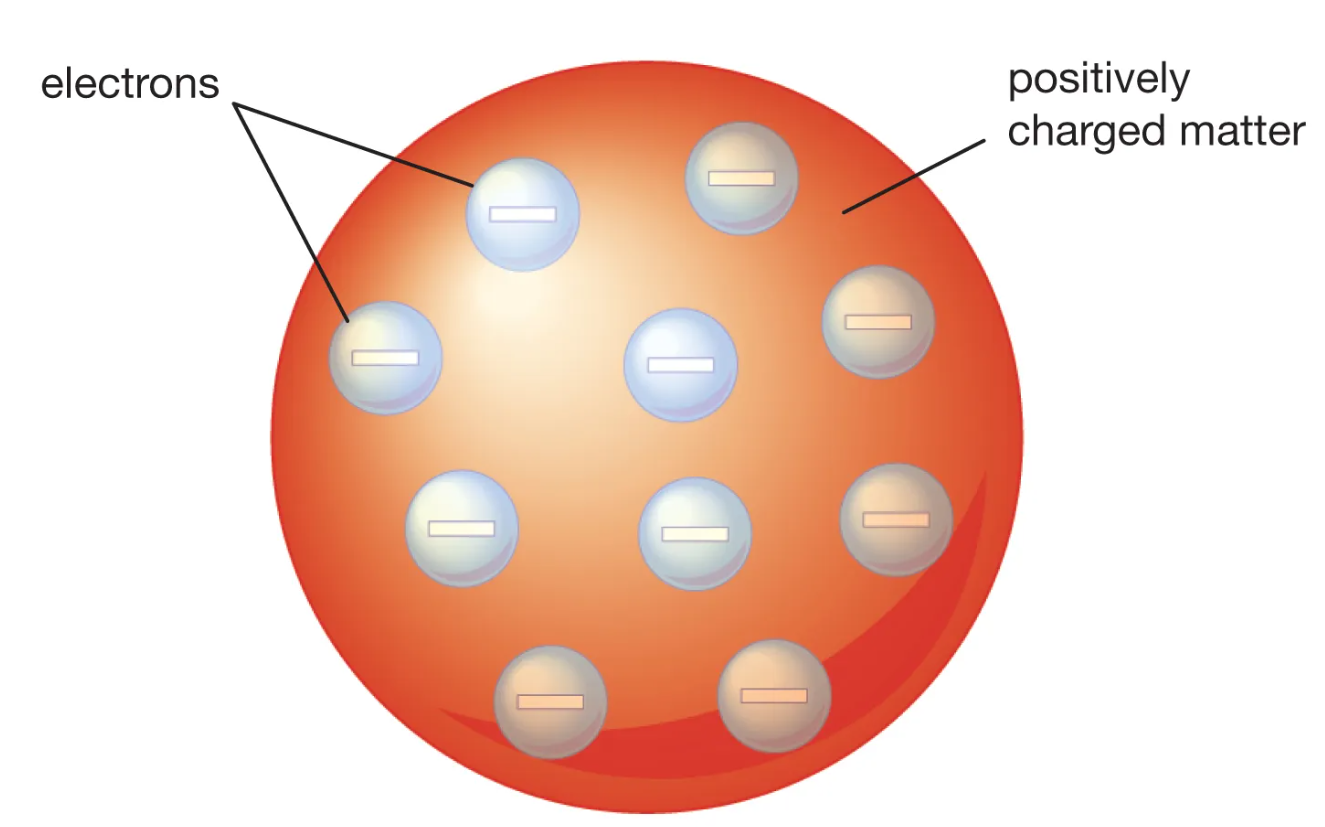
\includegraphics[trim={0 0  0 0cm} ,clip,width=.982\textwidth]{Introduction/plumb.png}
                        \caption{{Thomson model of atom, with negatively charged electrons embedded in positively charged ball \\
                        {\myfont{\tiny  [Britannica:Thomson Atomic Model]   }}}}
                        %britannica.com/science/Thomson-atomic-model
                        \label{fig:plumpudding}
                    \end{figure}
            
    \end{columns}
\end{frame}


\begin{frame}{Brief History of the Proton}


   \begin{columns}
        \column{0.69\textwidth}
        
              \begin{itemize}
                    \setlength\itemsep{1em}
                    \item  \textbf{$\sim$ 1911: Discovery of the Nucleus} - Scattering $\alpha$ particles off gold foil yielded significant backscatter, indicating small, dense nucleus  {\myfont{\tiny  [Wikipedia:Geiger-Marsden]   }}
                    \item \textbf{$\sim$ 1919: Discovery of the Proton} - Proposed by Rutherford after $\alpha$ particle scattering experiments off atoms {\myfont{\tiny  [E. Rutherford doi:10.1080/14786431003659230]   }}
                    \item \textbf{$\sim$1961: Discovery of Quarks} - Electron scattering experiments provided evidence consistent with the proton being a composite object of point-like constituents 
                    \end{itemize}

        \column{0.31\textwidth}
                    %\vspace{2cm}
                    \begin{figure}
                        \centering
                        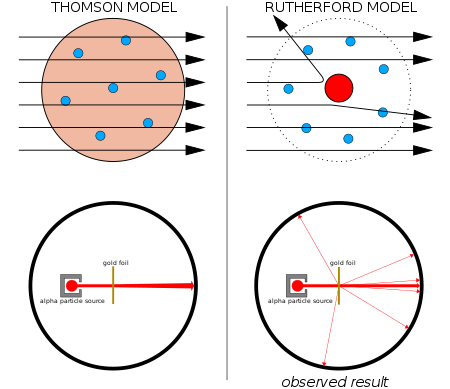
\includegraphics[trim={9cm 8cm  0 0cm} ,clip,width=.6\textwidth]{Introduction/rutherfordscattering.png}
                        \caption{     {\myfont{\tiny  [Wikimedia:Geiger-Marsden Exp.]   }}}
                        %https://upload.wikimedia.org/wikipedia/commons/thumb/8/89/Bohr_model_Hydrogen.svg/1280px-Bohr_model_Hydrogen.svg.png
                        \label{fig:plumpudding1}
                    \end{figure}
                    \vspace{-1cm}
                     \begin{figure}
                        \centering
                        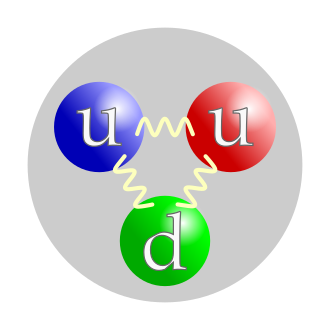
\includegraphics[trim={0 0  0 0cm} ,clip,width=.65\textwidth]{Introduction/proton_quarks.png}
                        \caption{
                        {\myfont{\tiny  [Wikimedia:Proton Quark Structure]   }}}
                        %https://upload.wikimedia.org/wikipedia/commons/thumb/8/89/Bohr_model_Hydrogen.svg/1280px-Bohr_model_Hydrogen.svg.png
                        \label{fig:plumpudding2}
                    \end{figure}
            
    \end{columns}
\end{frame}


\begin{frame}{The Proton is Now Well-Understood}
   \begin{columns}
        \column{0.69\textwidth}
        Protons are:
              \begin{itemize}
                    \setlength\itemsep{1em}
                    \item \textbf{Spin 1/2}
                    \item \textbf{Stable}: mean lifetime $>$ 1E34 years 
                    \item \textbf{Lightweight}: 938.272088 MeV; lightest baryon\\
                     {\myfont{\tiny  [n.b. 1 eV = 1.8E-36 kg]   }}
                    \item \textbf{Small}: radius $\sim$ 0.85 fm\\
                         \begin{itemize}
                            \item If protons were scaled to the size of pingpong balls,\\
                            atoms would be $\sim$ 4 football fields across,\\
                            humans would be $\sim$ diameter of the inner solar system
                        \end{itemize}
                    \end{itemize}
                    
                    
        \column{0.31\textwidth}
                    %\vspace{2cm}
                    \begin{figure}
                        \centering
                        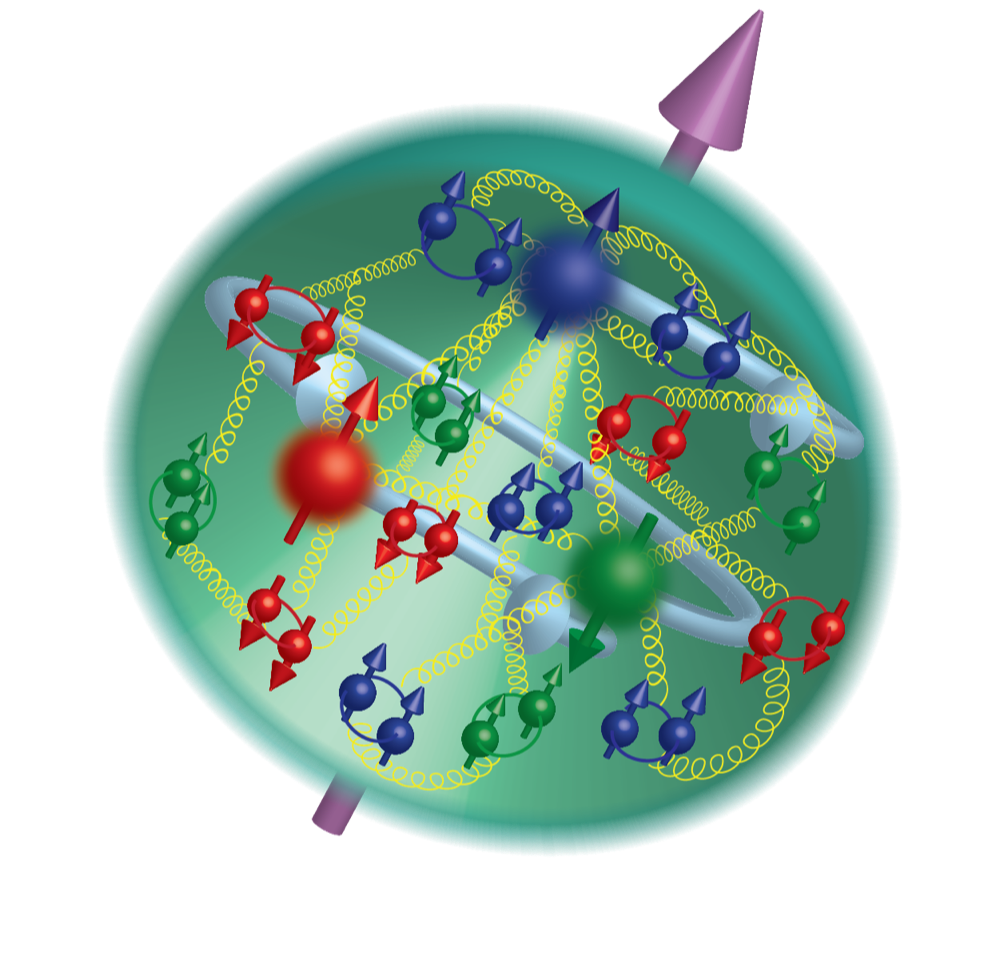
\includegraphics[trim={0 0  0 0cm} ,clip,width=.982\textwidth]{Introduction/modernproton.png}
                        \caption{                       {\myfont{\tiny  [Argonne National Lab]   }}}
                        %https://www.anl.gov/article/getting-up-to-speed-on-the-proton
                        \label{fig:modernproton1}
                    \end{figure}
            
    \end{columns}
\end{frame}


\begin{frame}{The Proton is \textbf{NOT} well-understood - Testbed for Physics}
    Macroscopic features are well measured, but many properties remain to be understood
    \begin{columns}

           \column{0.31\textwidth}
                    %\vspace{2cm}
                    \begin{figure}
                        \centering
                        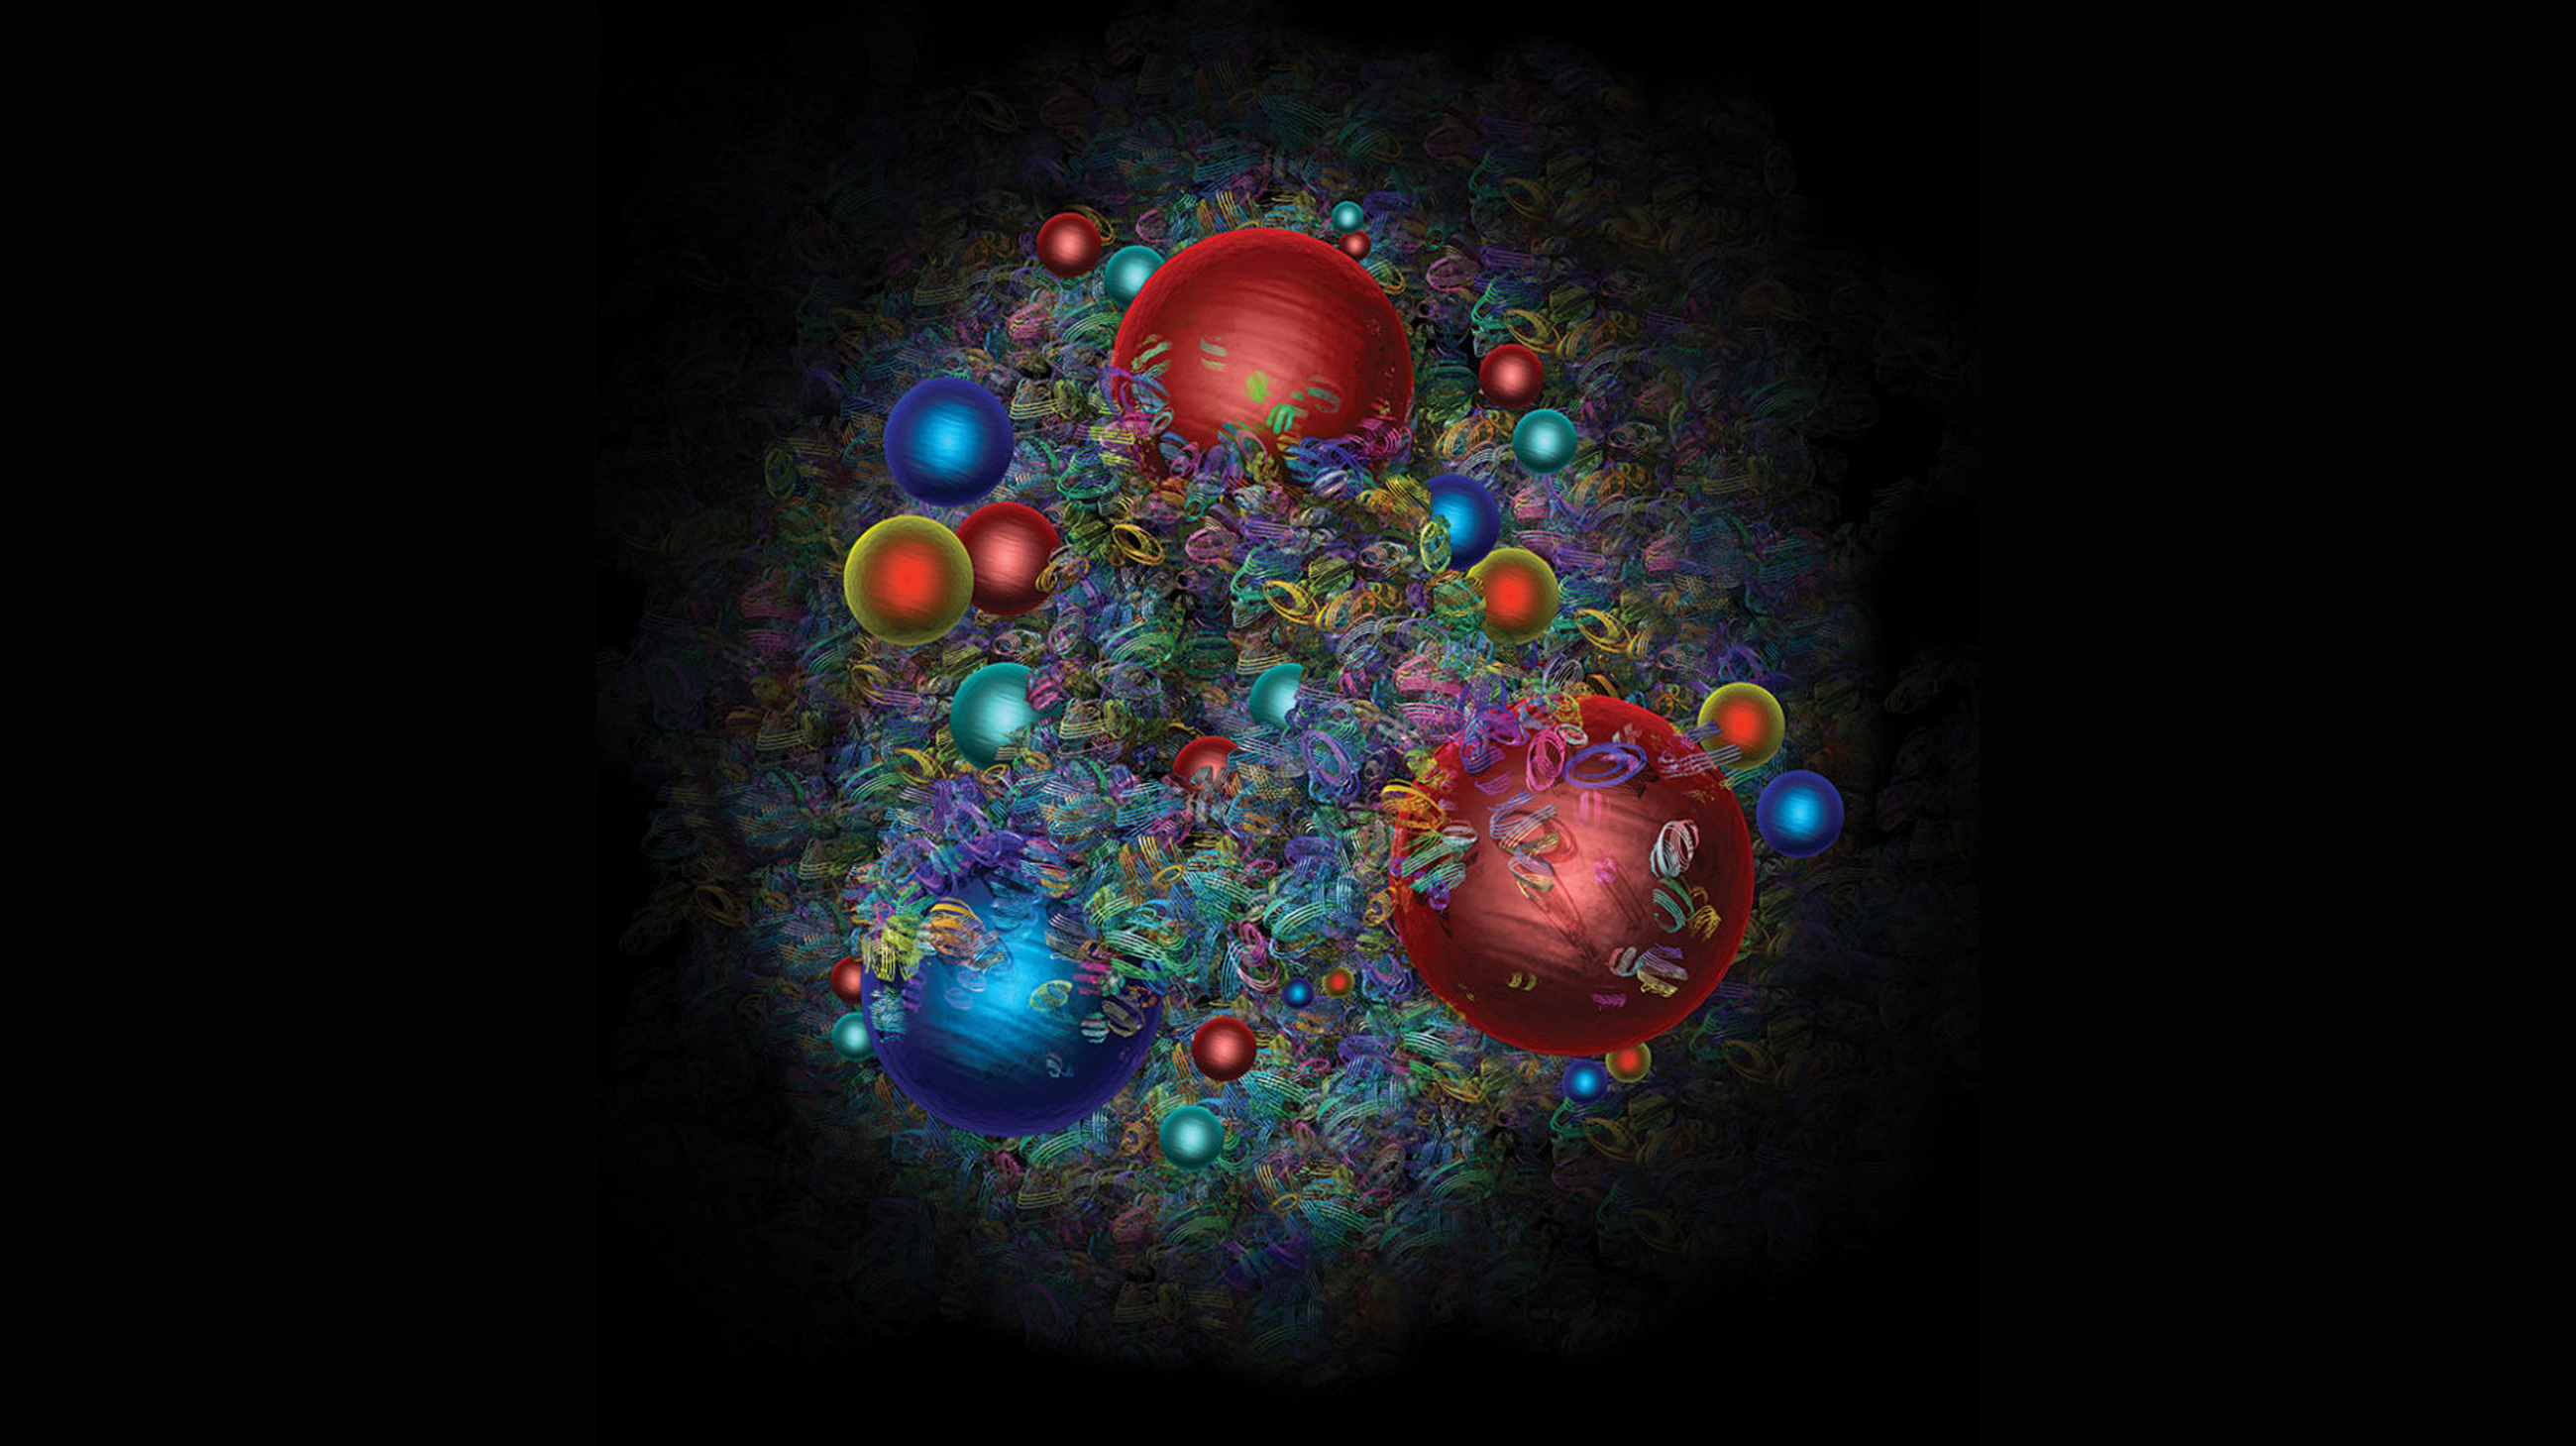
\includegraphics[trim={25cm 5cm  25cm 5cm} ,clip,width=.982\textwidth]{Introduction/quanta_protons.jpg}
                        \caption{                       {\myfont{\tiny  [Quanta Magazine 20190911]   }}}
                        %https://www.anl.gov/article/getting-up-to-speed-on-the-proton
                        \label{fig:modernproton}
                    \end{figure}
                    
        \column{0.69\textwidth}
       
              \begin{itemize}
                    \setlength\itemsep{1em}
                     \item \textbf{Proton Spin Crisis}: Where does the proton's spin come from? 1987 measurement showed valence quarks only contribute  a small percent to overall proton spin
                     \item \textbf{Proton Decay}: Popular Beyond-Standard-Model theories predict the proton to decay, but never has been observed
                     \item \textbf{Proton Radius Puzzle}: (possibly resolved) discrepancy in proton charge radius between experimental methods
                      \end{itemize}

            \quad \quad \quad  {\myfont{\tiny \quad \quad \quad [Proton Puzzles, Nat Rev Phys, 2021]   }}
                
            
    \end{columns}
\end{frame}


\begin{frame}{Probing the Proton: Accelerators as Electron Femtoscopes}
Imaging limited by diffraction ($\sim \frac{\lambda}{2}$) $\rightarrow$ scale set by $\lambda = \frac{hc}{pc}$ with hc = 1200 eV nm
  \begin{columns}

           \column{0.33\textwidth}
                        %\vspace{2cm}
                       \centering 
                    Optical Microscope
                    \begin{figure}
                        \centering
                        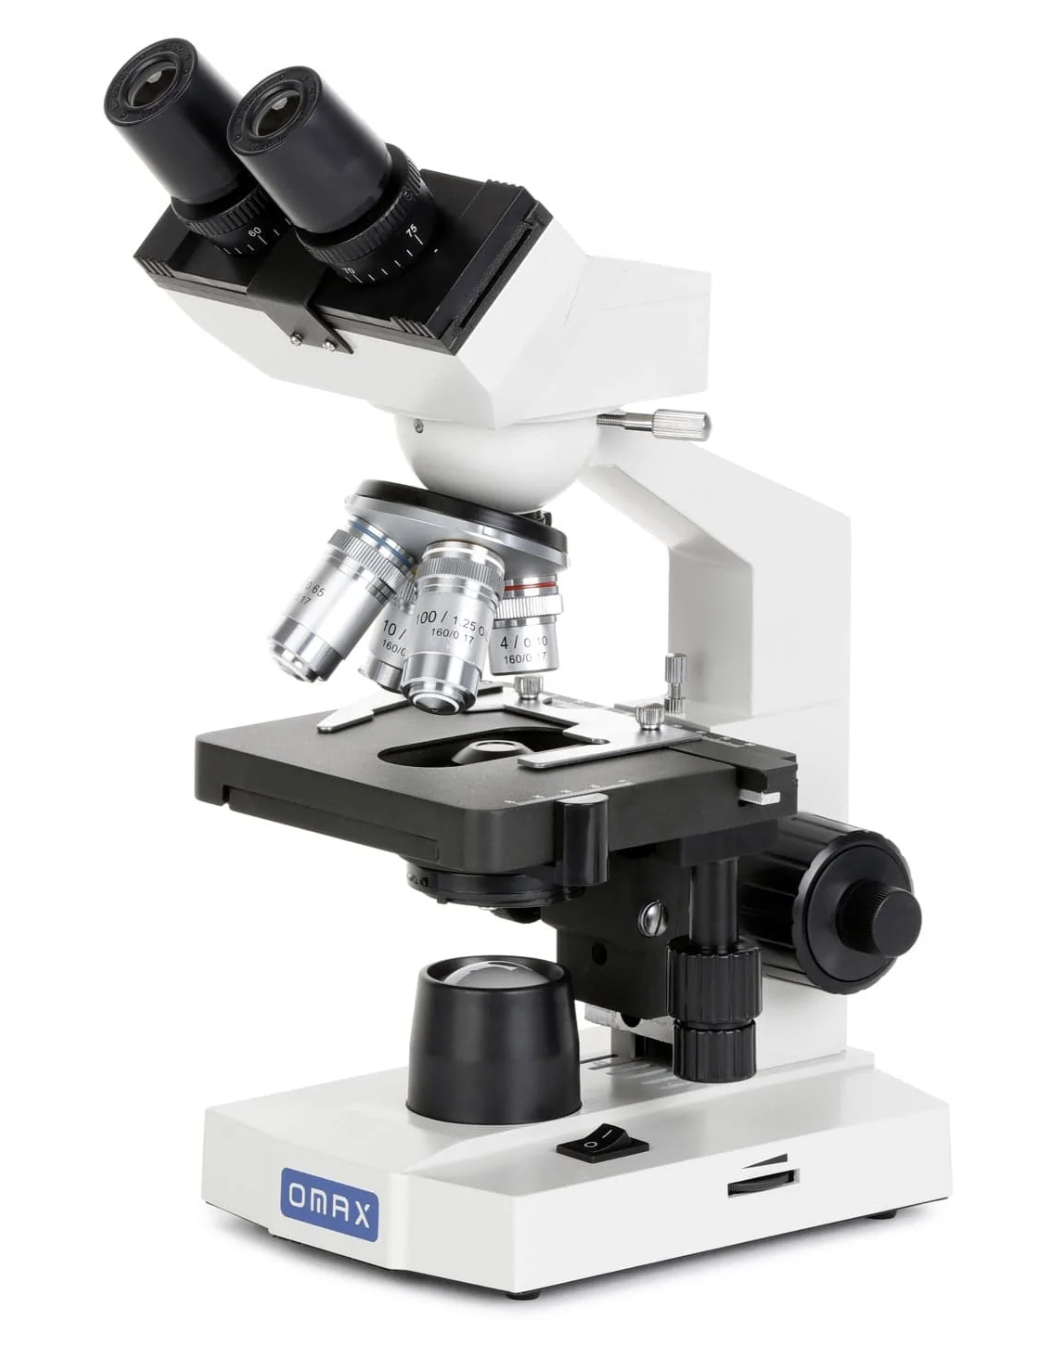
\includegraphics[trim={0 1cm 0 0cm} ,clip,width=.67\textwidth]{Introduction/optmic.png}
                        %\caption{                       {\myfont{\tiny  [Quanta Magazine 20190911]   }}}
                        %https://www.anl.gov/article/getting-up-to-speed-on-the-proton
                        \label{fig:modernproton}
                    \end{figure} 
                     3 eV $\rightarrow$ $\lambda$ $\sim$ 400 nm\\
                     {\myfont{\tiny \quad \quad \quad [n.b. ex. mic for bio]   }}
        \column{0.33\textwidth}
        \centering
        Electron Microscope
                    \begin{figure}
                        \centering
                        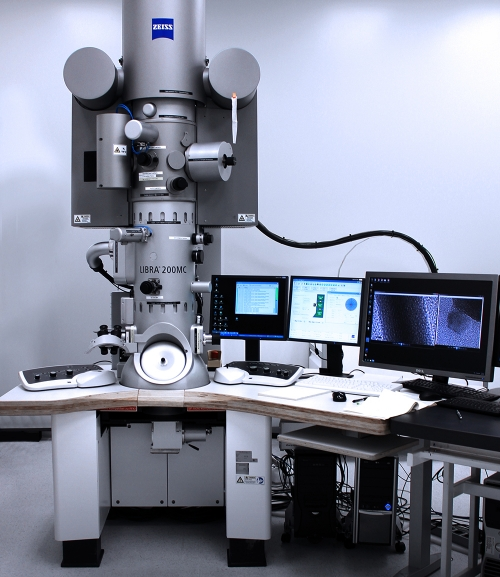
\includegraphics[trim={0 0 0 0} ,clip,width=.77\textwidth]{Introduction/elecmic.jpg}
                        %\caption{                       {\myfont{\tiny  [Quanta Magazine 20190911]   }}}
                        %https://www.anl.gov/article/getting-up-to-speed-on-the-proton
                        \label{fig:modernproton}
                    \end{figure} 
             10 keV $\rightarrow$ $\lambda$ $\sim$ 0.01 nm
                    
         \column{0.33\textwidth}
         \centering
         Electron Accelerator
                    \begin{figure}
                        \centering
                        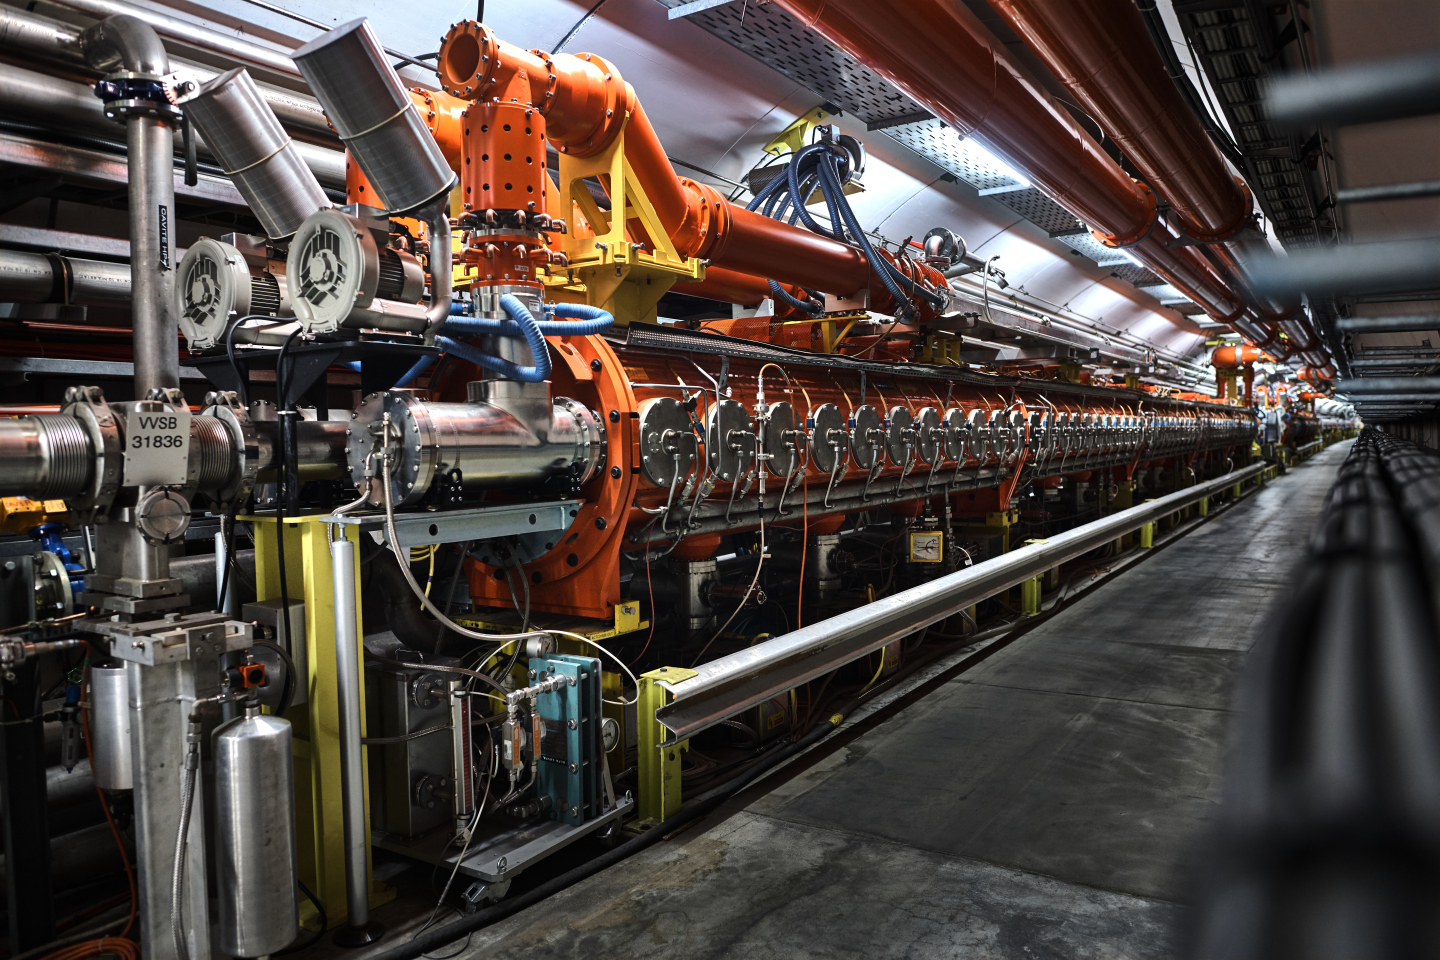
\includegraphics[trim={2cm 0 2cm 0} ,clip,width=.82\textwidth]{Introduction/elecfemt.jpg}
                        %\caption{                       {\myfont{\tiny  [Quanta Magazine 20190911]   }}}
                        %Source  https://home.cern/science/engineering/accelerating-radiofrequency-cavities
                        \label{fig:modernproton}
                    \end{figure} 
            10 GeV $\rightarrow$ $\lambda$ $\sim$ 0.1 fm
                    
         
    \end{columns}
\end{frame}

\begin{frame}{Proton can only be Indirectly Imaged}
 Rely on scattering, see what comes out.  [include slides from Or Hen]
 Specific reactions encode specific pieces of information of proton structure - e.g. quark momentum or spatial distributions
 
  1\q determines the spatial resolution
                     pressure very high
                    Translation scale: $\hbar c$ = 0.2 GeV fm - 
                    Can't directly measure distributions, instead have to measure reaction rates, and infer distributions from obersved rates - cross section
                    1/x determines the shutter speed
  \begin{itemize}
                    \item PDFs - 1D structure
                    \item GPDs - 3D structure 
                    \item sidis, 
    \end{itemize}
    
\end{frame}



\begin{frame}{Proton Structure: Distribution Functions}

 Rely on scattering, see what comes out.  [include slides from Or Hen]
  1\q determines the spatial resolution
  light microscope vs electron microscope vs femtomicroscope
                     pressure very high
                    Translation scale: $\hbar c$ = 0.2 GeV fm - 
                    Can't directly measure distributions, instead have to measure reaction rates, and infer distributions from obersved rates - cross section
                    1/x determines the shutter speed
  \begin{itemize}
                    \item PDFs - 1D structure
                    \item GPDs - 3D structure 
                    \item sidis, 
    \end{itemize}
    
\end{frame}



\begin{frame}{Theory:Experiment Relation: Xi and DVEP}
DVCS, DVMP, how we get information from scattering
\end{frame}


\begin{frame}{Experiment Overview}
Describe how we are going to measure this process
Gonna take an electron, speed it up [accelerator], ram it into proton and detect what comes out [experiment and detectors], going to reconstruct what happened [analysis]
\end{frame}


\begin{frame}{Process Background}

    %\vspace{-.5cm}
         \begin{columns}[t, onlytextwidth]
         
          \column{0.35\textwidth}
            \centering Deeply Virtual $\pi^0$ Production\\
            \centering(\textcolor{alert}{DV$\pi^o$P})
            \begin{center}
                
                $e+p \rightarrow$ \\
                $e'+p' + \pi^0 \rightarrow$\\
                $e' + p' + \gamma_1 + \gamma_2$ 
            \end{center}
            
            
            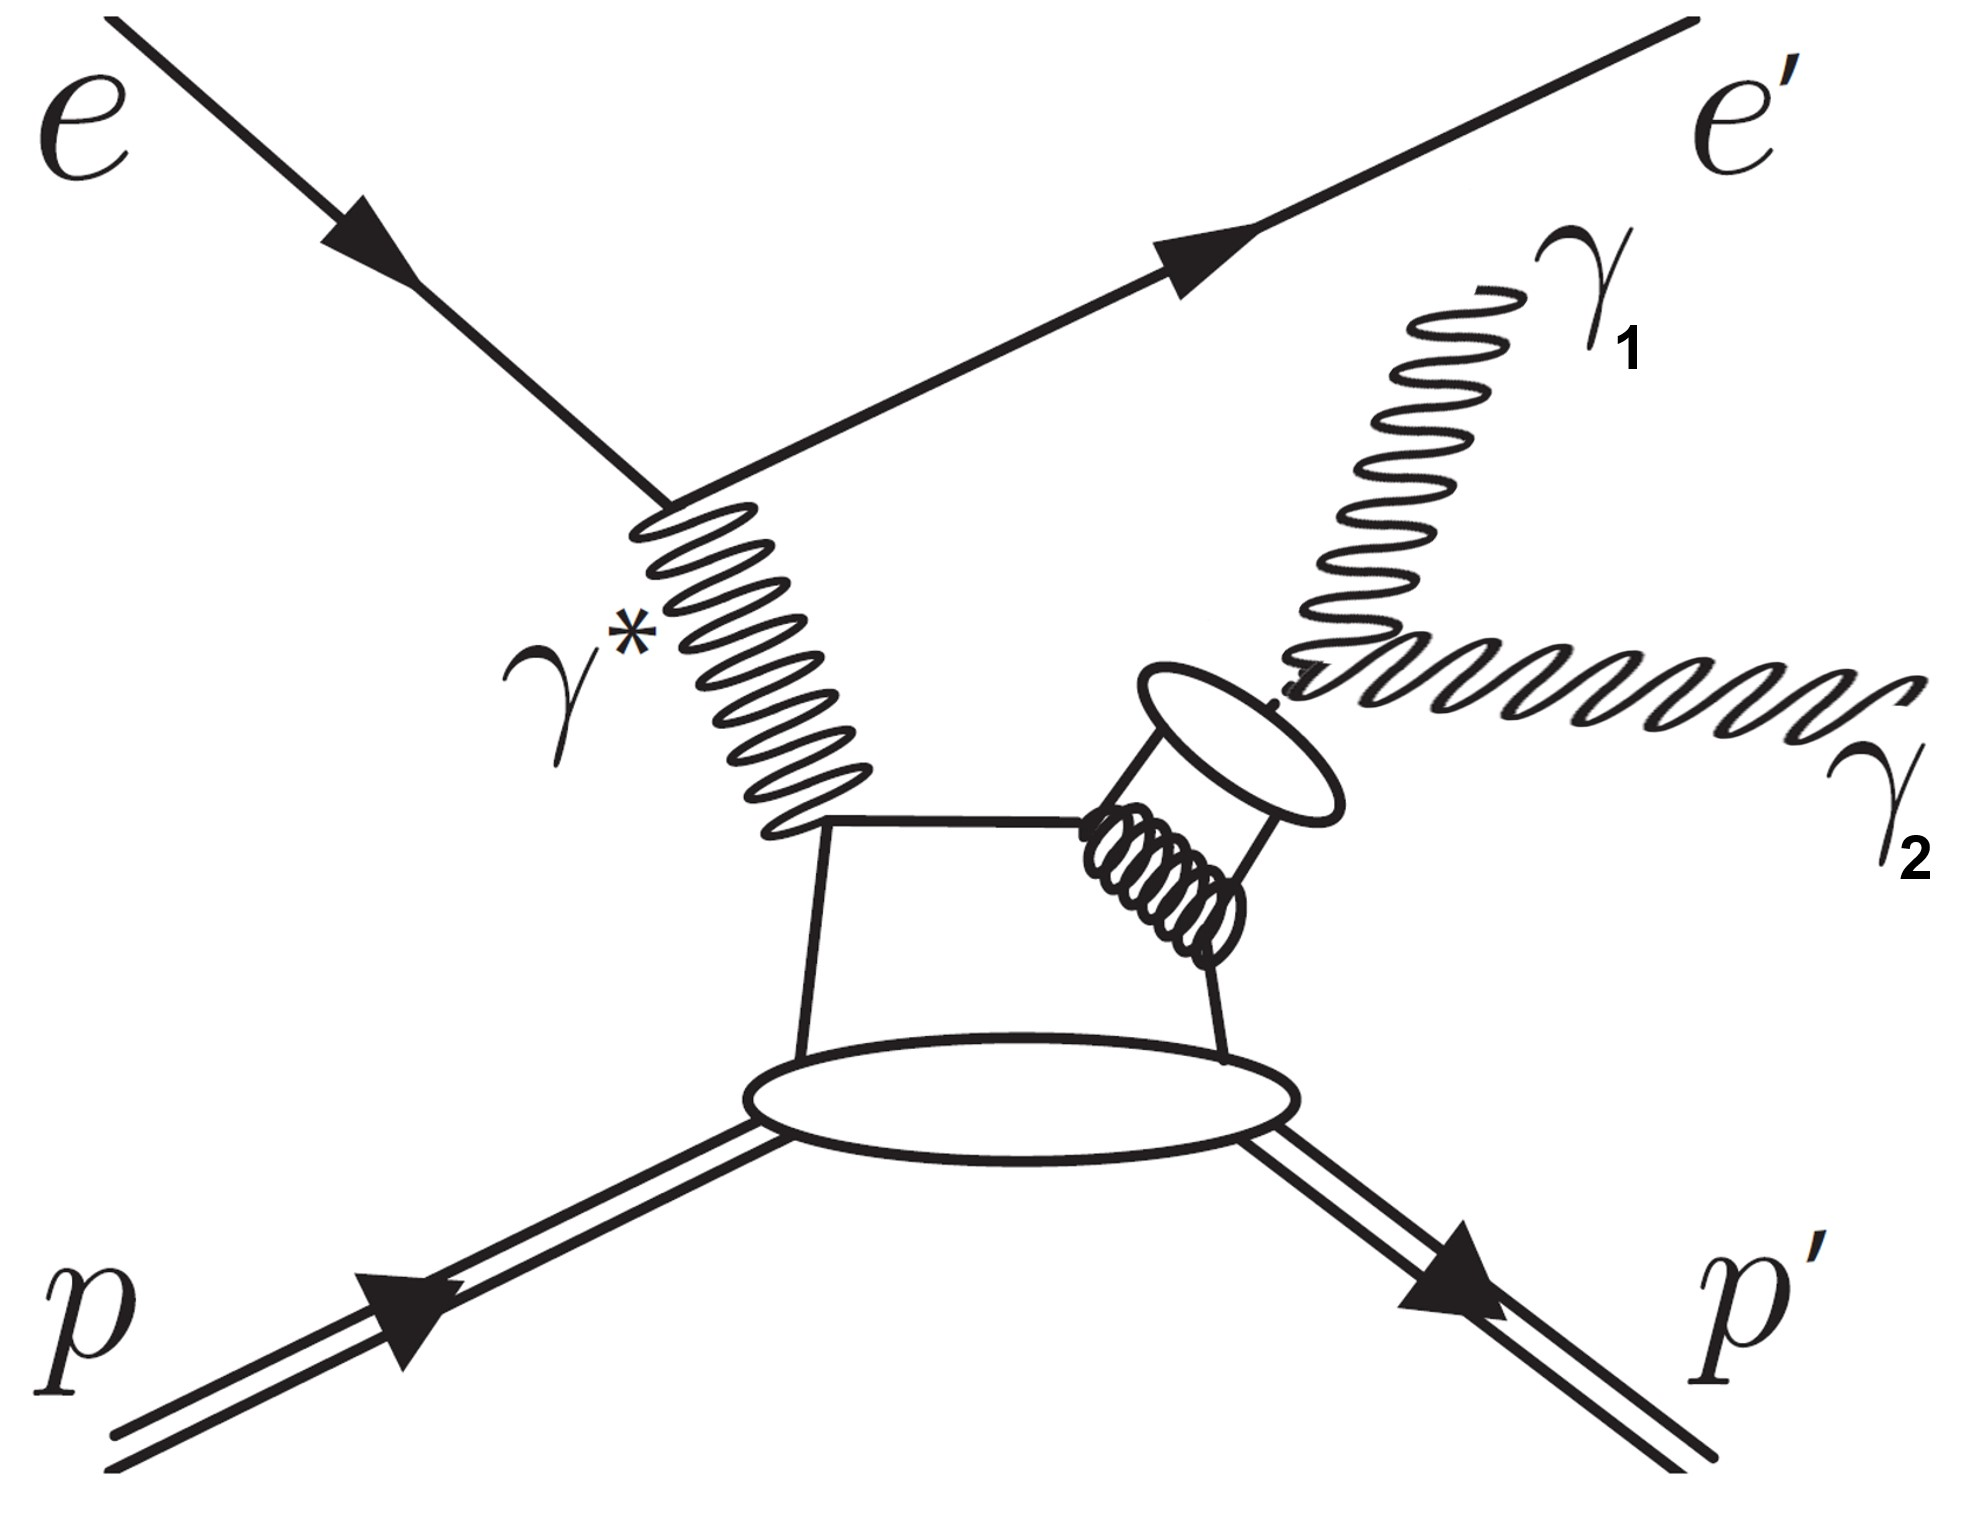
\includegraphics[trim={0 0 0 0cm} ,clip,width=.95\textwidth]{DNP/dvPiP_Feynman_diagram_2.jpg}
            
            
            
            \column{0.65\textwidth}
                \begin{itemize}
                    \setlength\itemsep{1em}
                    \item 4-fold differential cross section $\frac{d\sigma}{d\textcolor{alert}{Q^2}d\textcolor{alert}{x_B}d\textcolor{alert}{t}d\textcolor{alert}{\phi}}$ expressed in terms of:
                        \begin{itemize}
                        \setlength\itemsep{0.5em}
                            \item Virtual photon 4-momentum:  \textcolor{alert}{$Q^2$} $\equiv$  $-(p_e-p_{e'})^2$
                            \item Bjorken x: \textcolor{alert}{$x_B$} $\equiv$ $\frac{Q^2}{2p_p\cdot(p_{e}-p_{e'})}$
                            \item Momentum transfer: \textcolor{alert}{-t} $\equiv$ $-(p_{p'}-p_p)^2$
                            \item Angle between lepton \& hadron planes: \textbf{\textcolor{alert}{$\phi$}} = 
                            
                             \begin{columns}[t, onlytextwidth]
         
          \column{0.6\textwidth}
             \begin{center}
                            
                            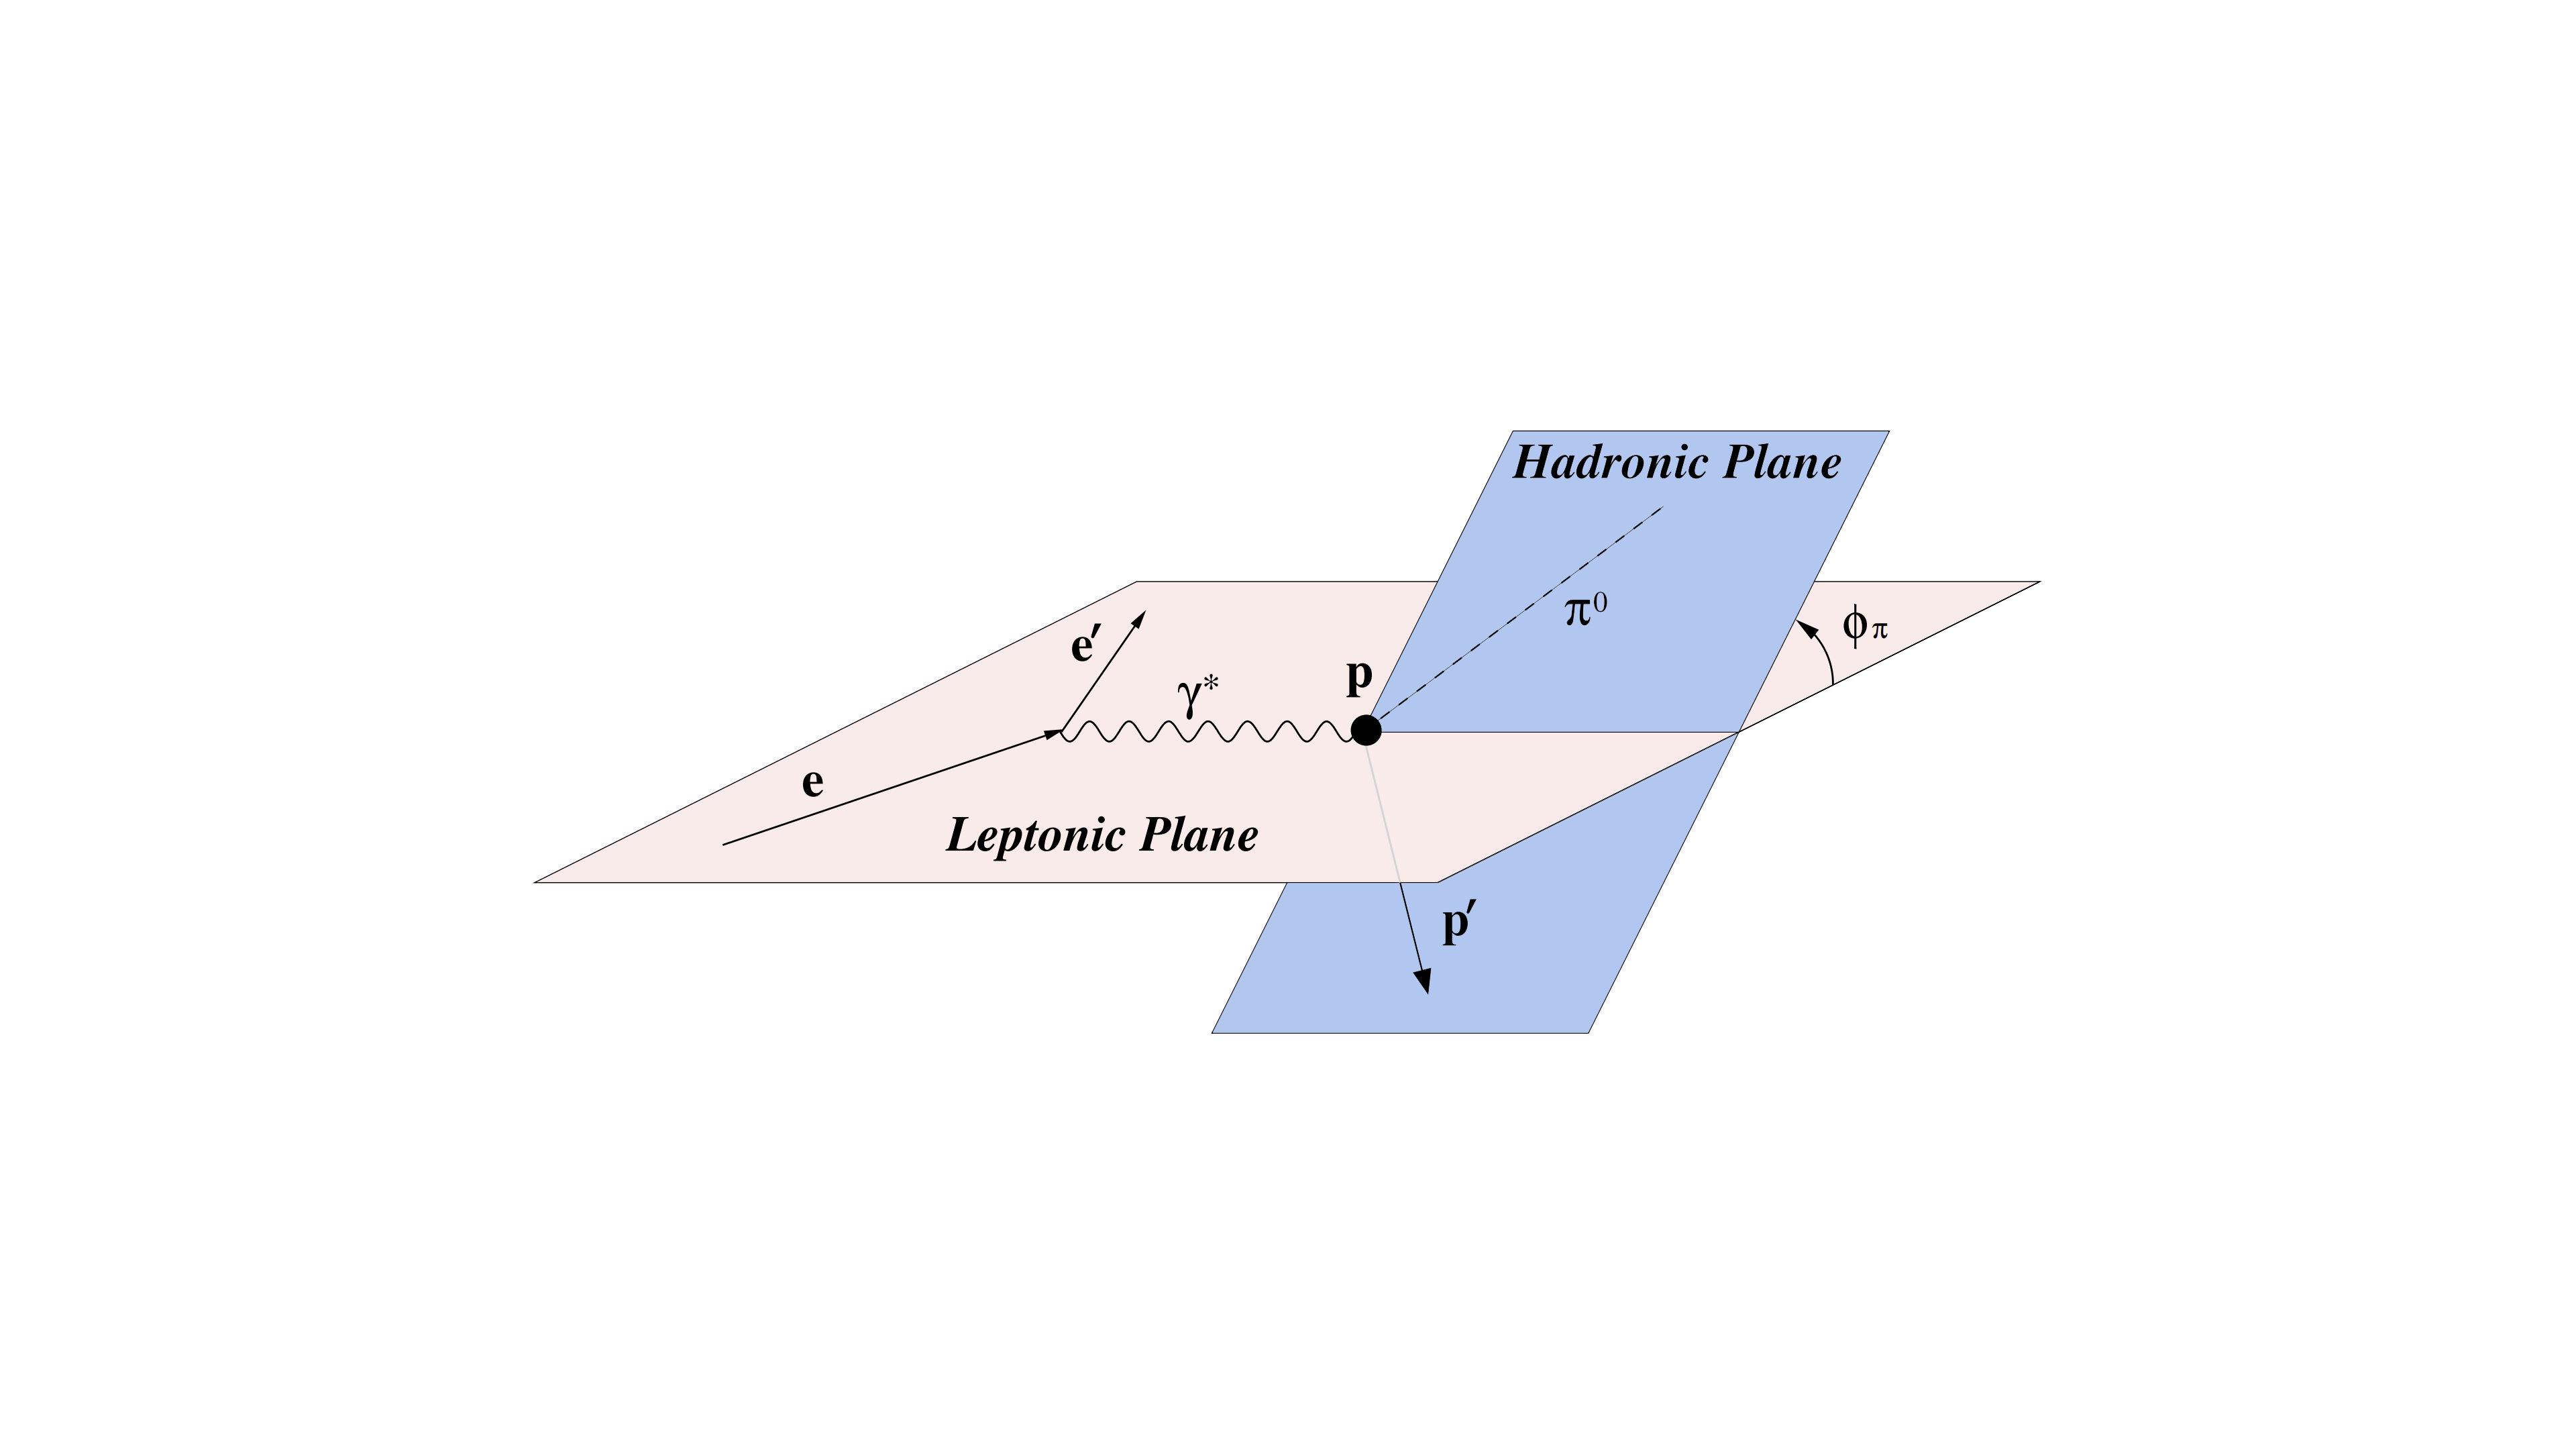
\includegraphics[trim={10cm 8cm 10cm 8cm} ,clip,width=.96546725995\textwidth]{DNP/lept_had_planes.png}
                            \end{center}
            \column{0.4\textwidth}
            \footnotesize{$\cos^{-1} \left( \frac{ \left(p_{e} \times p_{e'} \right) \cdot \left( p_{p'} \times p_{\gamma^*} \right) }{ \lVert p_{e} \times p_{e'} \rVert \: \lVert p_{p'} \times p_{\gamma^*} \rVert} \right)$}
          
          \vspace{1.5cm}
          {\myfont{\tiny     \textcolor{white}{lllllll} Images from S. Lee, A. Kim   }}
         \end{columns}
                            
                        \end{itemize}
                                            
                    \item In DIS regime: W$>2$GeV, $Q^2$> 1GeV$^2$
                \end{itemize}
                
     
                               
        \end{columns}
\end{frame}    



\begin{frame}{Physics Motivation: $DV\pi^0P$ and GPDs}


    \vspace{-.01cm}
   
    The cross section for DV$\pi^0$P has theoretically linked to Generalized Parton Distributions (GPDs), which describe the 3D structure of the nucleon:\\
    \vspace{0.1cm}
 \scalebox{0.735}{%
    $
         \frac{d^4\sigma_{\gamma^*p \rightarrow p'\pi^0}}{dQ^2dx_Bdtd\phi_{\pi}} =
         \Gamma (Q^2, x_B, E)
         \frac{1}{2\pi}
         \left\{ \left(  \textcolor{sigmaT}{\frac{d\sigma_T}{dt}}+\epsilon  \textcolor{sigmaL}{\frac{d\sigma_L}{dt}} \right)+
         \epsilon cos(2\phi)  \textcolor{sigmaTT}{\frac{d\sigma_{TT}}{dt}} + 
         \sqrt{2\epsilon(1+\epsilon)} cos(\phi)  \textcolor{sigmaLT}{\frac{d\sigma_{LT}}{dt}} \right\}
         \quad | \quad
         \Gamma (Q^2, x_B, E) = \frac{\alpha}{8\pi} \frac{Q^2}{m^2_pE^2}\frac{1-x_B}{x_B^3}\frac{1}{1-\epsilon}
    $
    }
    %\vspace{0.05cm}

    \begin{columns}
            \column{0.5\textwidth}
    

    \begin{center}
         The structure functions can be expressed in terms of GPDs:
    \end{center}
   
    %\vspace{0.05cm}
   
    \scalebox{0.80}{%   
    $      \textcolor{sigmaL}{\frac{d\sigma_{L}}{dt}} = 
    \frac{4\pi\alpha}{kQ^2}\left\{ \left( 1 - \xi^2 \right) 
    \lvert \langle \GPDHtildeEQ \rangle \rvert ^2 
    -2\xi^2 \Re \left[  \langle \GPDHtildeEQ \rangle ^* \langle \GPDEtildeEQ \rangle    \right] - \frac{t'}{4m^2}\xi^2
    \lvert \langle \GPDEtildeEQ \rangle \rvert ^2  \right\}$
    }\\
    
    \scalebox{0.80}{%   
    $      \textcolor{sigmaT}{\frac{d\sigma_{T}}{dt}} = 
    \frac{2\pi\alpha \mu_{\pi}^2}{kQ^4}
    \left\{ \left( 1 - \xi^2 \right) 
    \lvert \langle \GPDHTEQ \rangle \rvert ^2
    - \frac{t'}{8m^2}
    \lvert \langle \GPDETbarEQ \rangle \rvert ^2  \right\}$
    }\\
    
    \scalebox{0.80}{%   
    $     \textcolor{sigmaLT}{\frac{d\sigma_{LT}}{dt}} = 
    \frac{4\pi\alpha \mu_{\pi}}{\sqrt{2}kQ^3}
    \xi\sqrt{1-\xi^2}
    \frac{\sqrt{-t'}}{2m}
    \Re \left\{ 
     \langle \GPDHTEQ \rangle ^*
    \langle \GPDEtildeEQ \rangle   
    \right\}$
    }\\
    
    \scalebox{0.80}{%   
    $      \textcolor{sigmaTT}{\frac{d\sigma_{TT}}{dt}} = 
    \frac{4\pi\alpha \mu_{\pi}^2}{kQ^4}
    \frac{-t'}{16m^2}
    \langle \GPDETbarEQ \rangle^2   
    $
    }\\
    

   
 
    
    \column{0.5\textwidth}
    
    \centering 
    %\vspace{0.3cm}
    GPD Classification:\\\tiny{\textcolor{white}{lll}}\\
         %\vspace{0.1cm}
         \footnotesize
    \scalebox{0.95}{%  
    \begin{table}[H]
        \centering
        \begin{tabular}{@{} *{4}{c} @{}}
                \headercell{Nucleon \\ Polarization} & \multicolumn{3}{c@{}}{Quark Polarization}\\
                \cmidrule(l){2-4}
                & U & \textcolor{white}{lllll}L & T    \\ 
                \midrule
                  U  & \GPDH &                                   &  \GPDETbar \\
                  L  &                    &  \textcolor{white}{llll}\GPDHtilde &                                   \\
                  T  & \GPDE &                                   &  \GPDHT,\GPDHTtilde \\
            \end{tabular}\\
            
    \end{table}
    }
            
        \vspace{0.1cm}
        \footnotesize{\GPDETbar = 2*\GPDHTtilde+\GPDET\\}
    
    \end{columns}
    \vspace{0.2cm}
    
     \begin{columns}
            \column{0.15\textwidth}
            \column{0.7\textwidth}
   \centering
   In contrast to DVCS, DV$\pi^0$P allows access to chiral-odd GPDs, making it a distinct and valuable probe
   
             \column{0.15\textwidth}
   \end{columns}
   
   \vspace{0.1cm}

\end{frame}


    

    
\begin{frame}{\textbf{Analysis Goal}: Extract DV$\pi^o$P Cross Section}
    Extracting the cross section for the process will extend the CLAS6 work to a larger kinematic range with higher statistics
        \begin{columns}
            \column{0.5\textwidth}
            \begin{figure}[H]
            \centering
            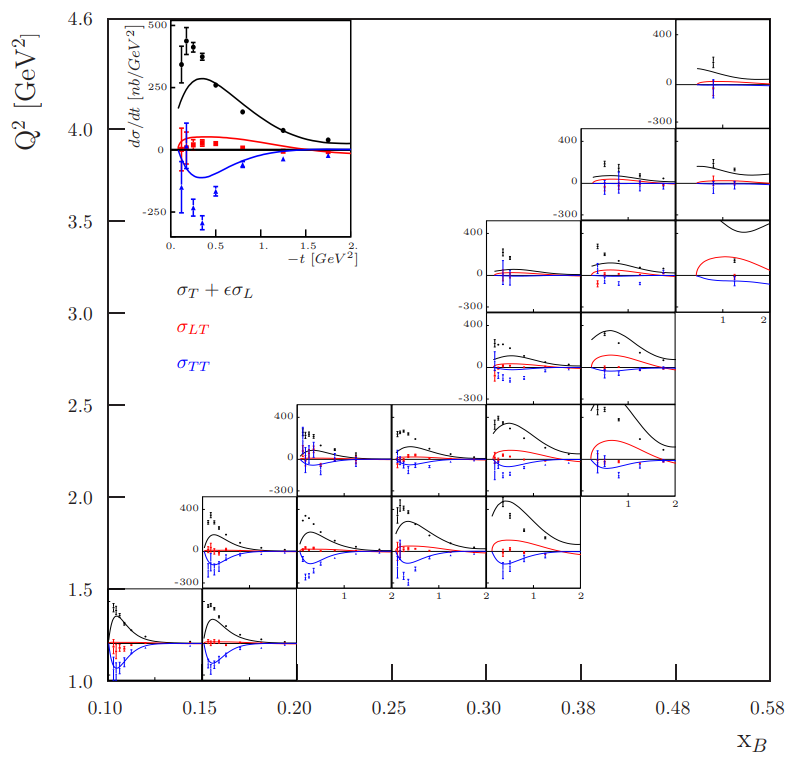
\includegraphics[width=.8\textwidth]{Pics/Goal/clas6CrossSection.png}
            \label{fig:clas6}
            \end{figure}
            
             \column{0.5\textwidth}
             \centering$Q^2$ vs. $x_B$ - CLAS12
             %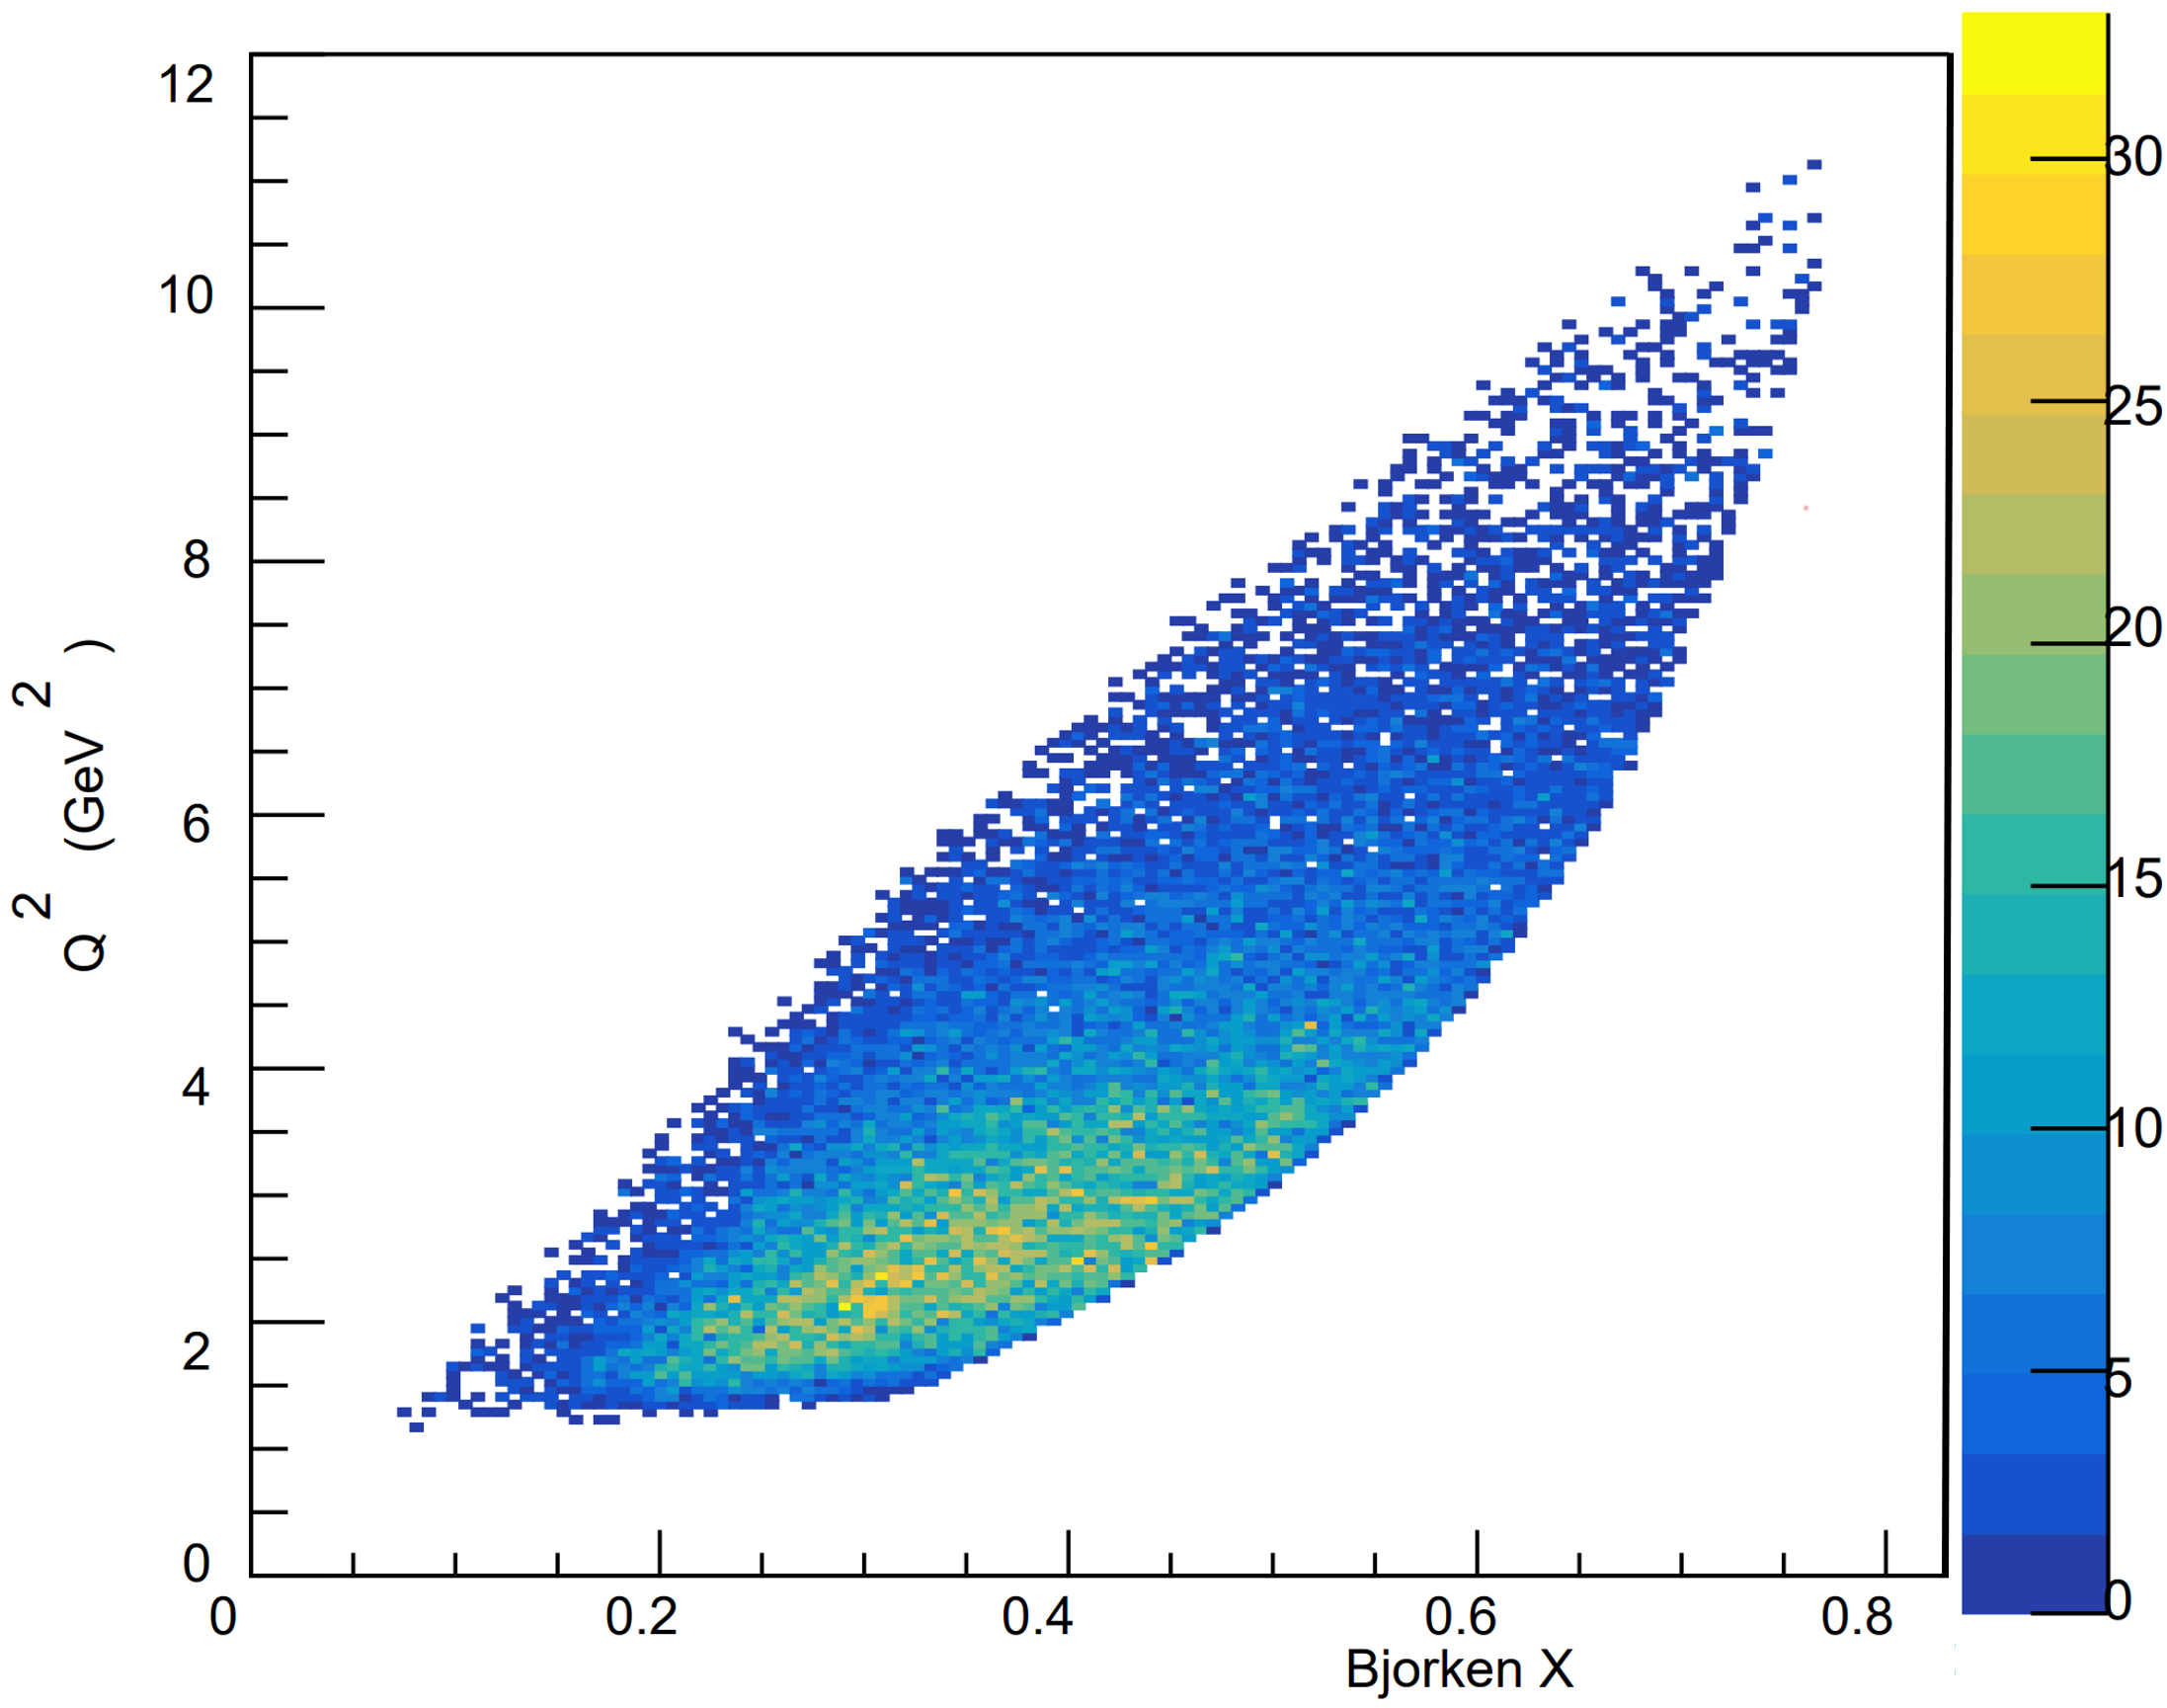
\includegraphics[width=.9\textwidth]{Pics/kinreach/bjorken_x_cropped.png}
             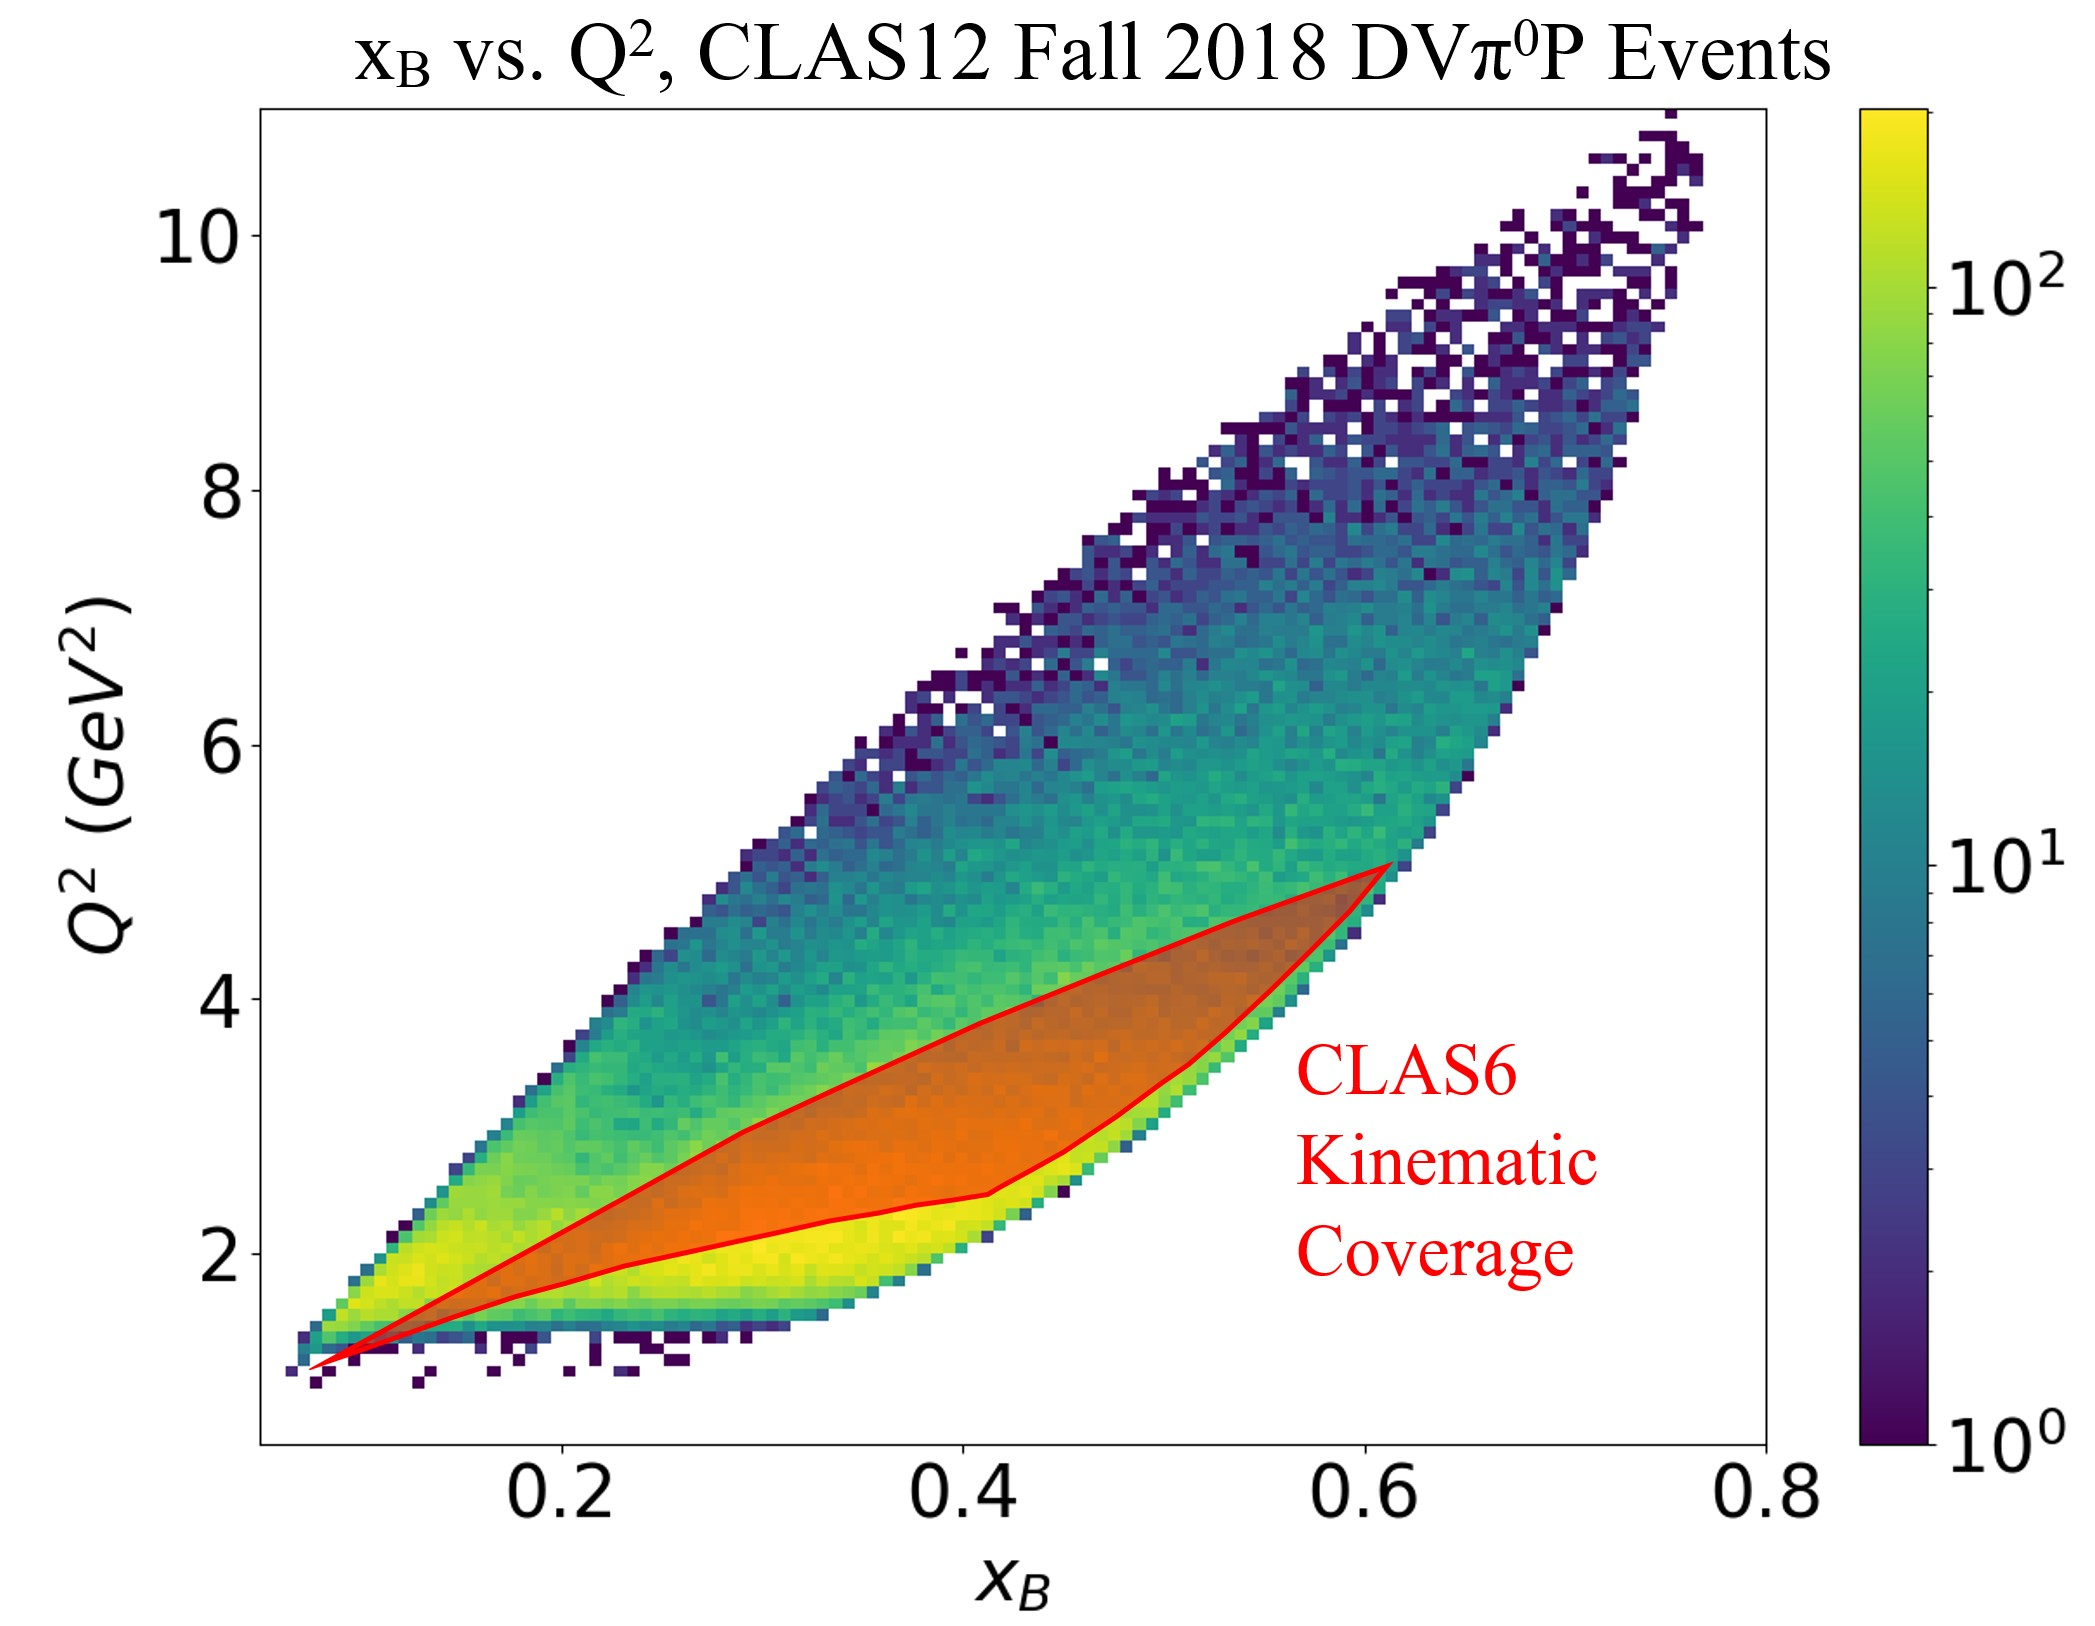
\includegraphics[trim={0 0 0 1.8cm} ,clip,width=.9725995\textwidth]{APS_2022/clas12_vs_clas6_kinematic_coverage.jpg}
    \end{columns}
    
    {\myfont{\tiny     I. Bedlinskiy et al., PRC, 90, 025205     (2014)   }}

\end{frame}


\begin{frame}{Jefferson Lab 10.6 GeV CEBAF Accelerator} \label{frame:datasets1}
        Thomas Jefferson National Accelerator Facility - Newport News, VA
        
        \begin{columns}[t, onlytextwidth]
            \column{0.5\textwidth}
                %\vspace{1cm}
                \begin{figure}[t!]
                    %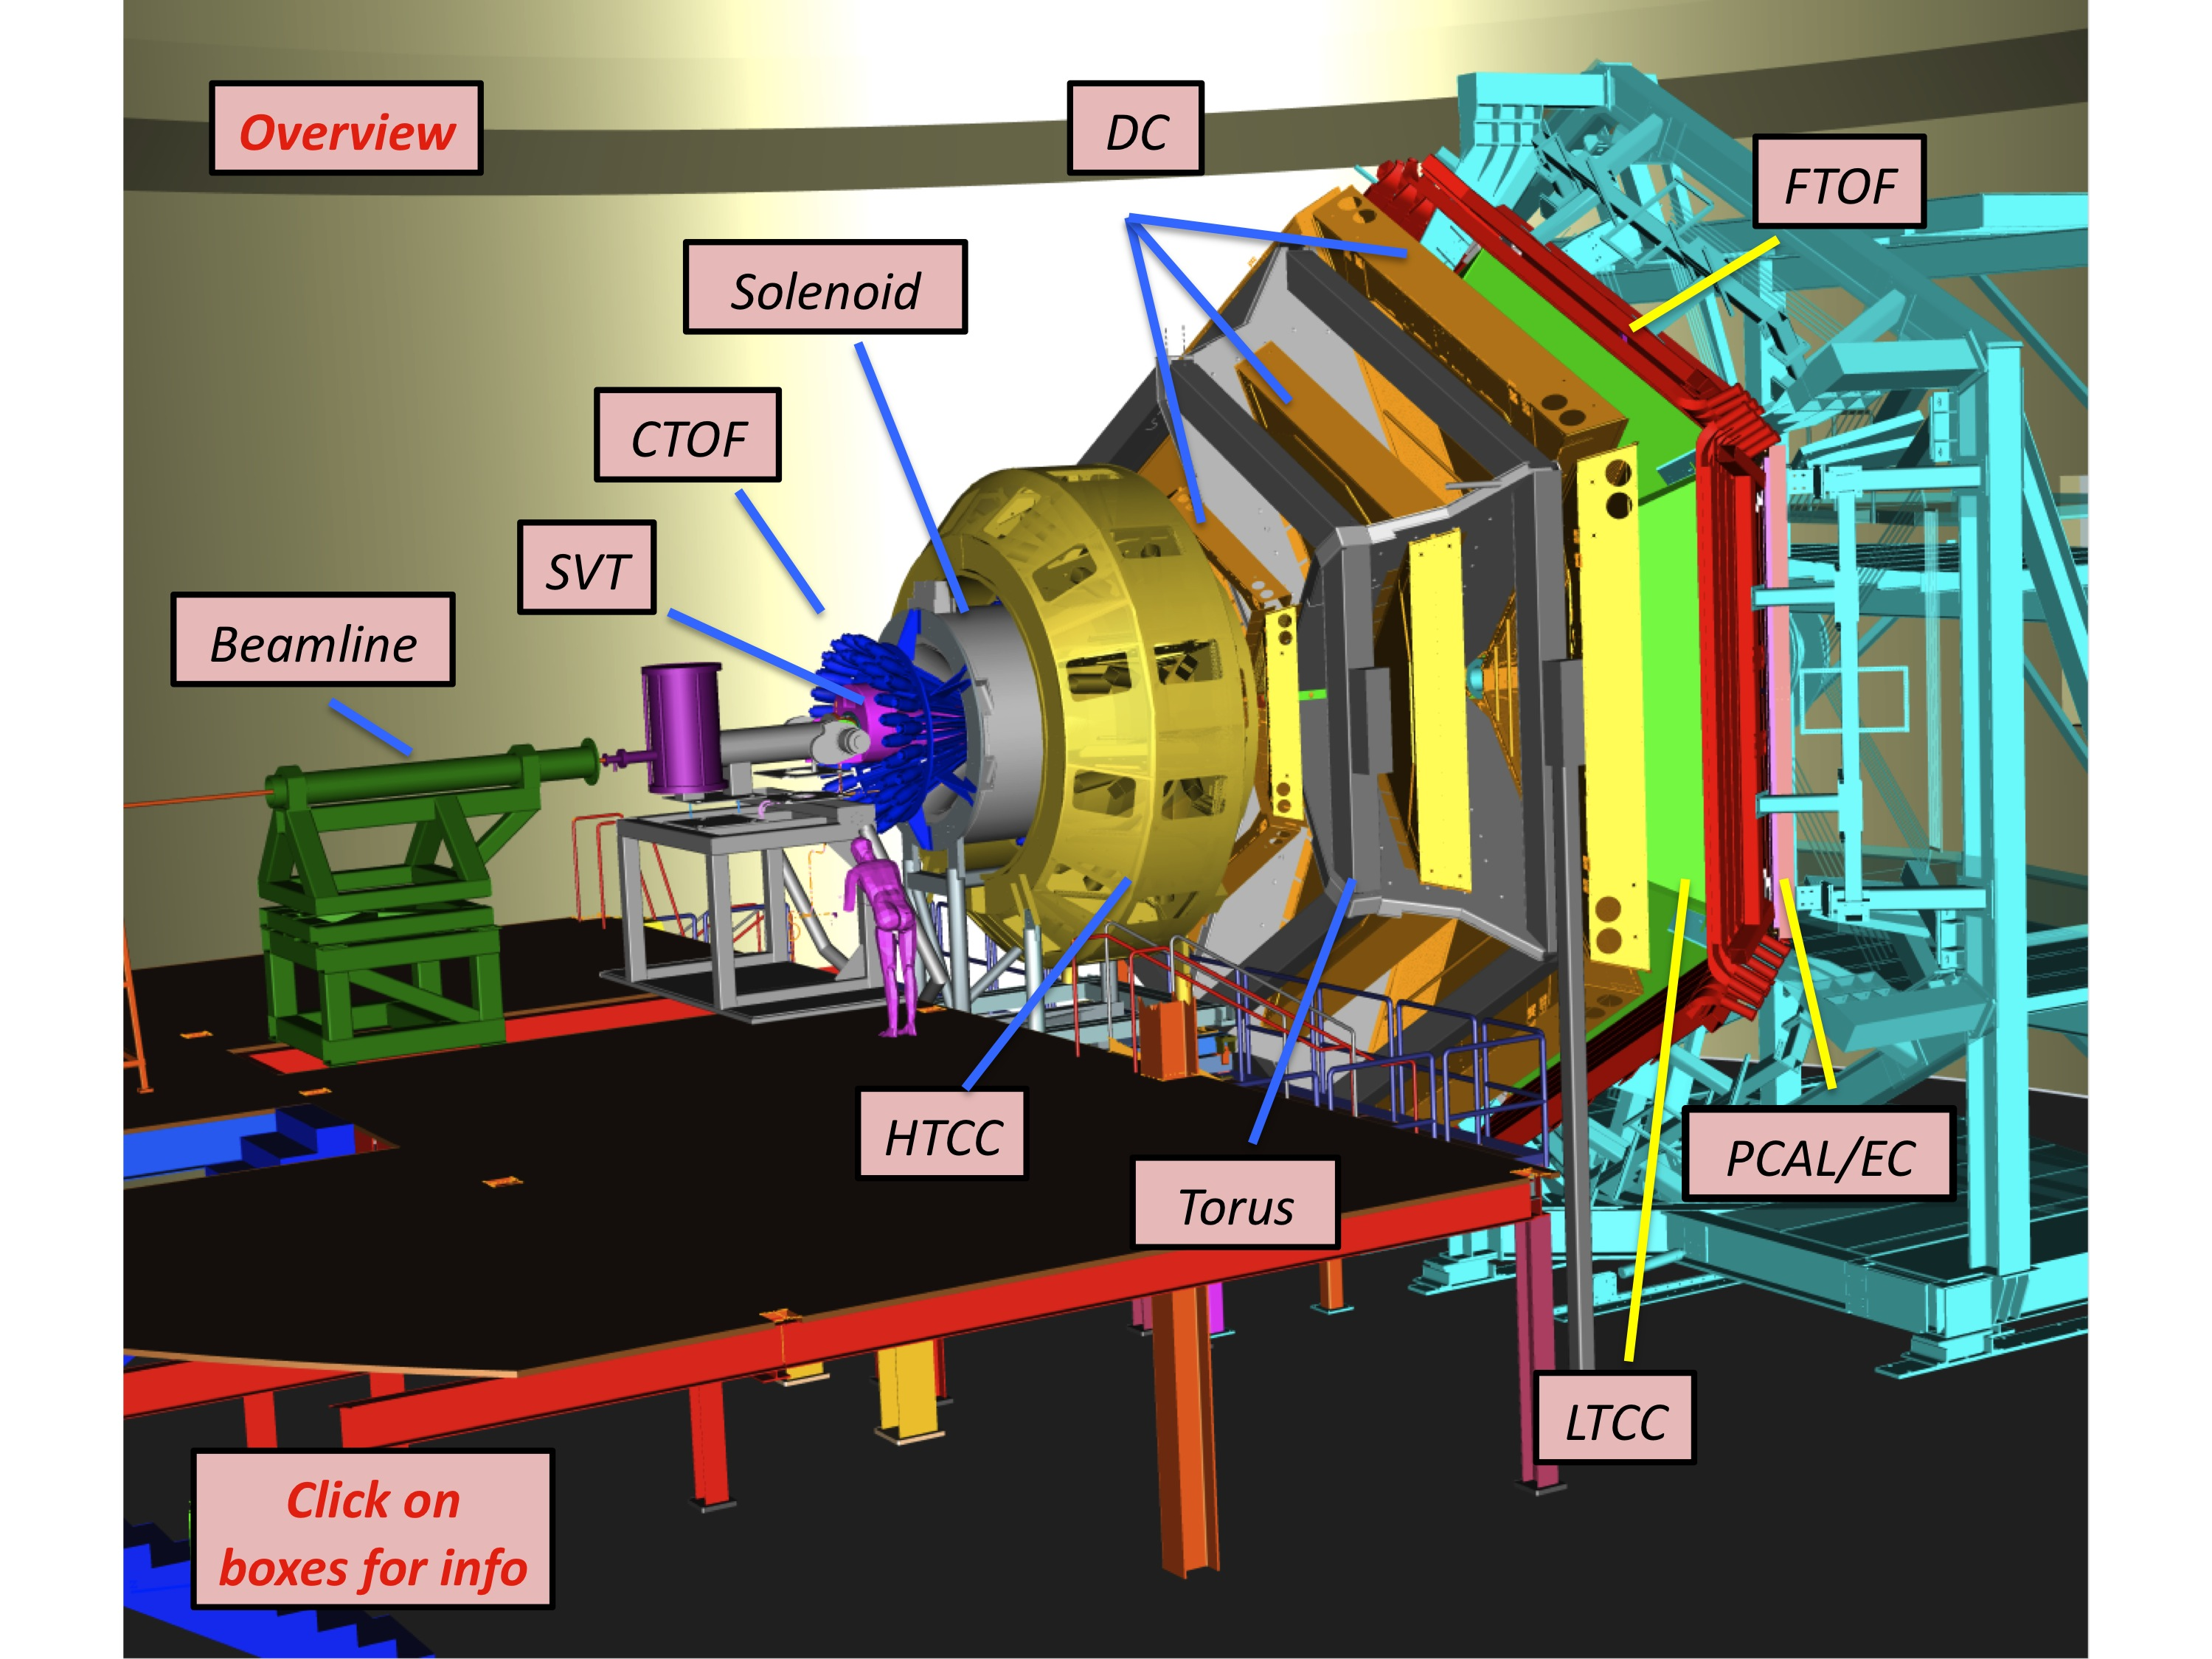
\includegraphics[height=\dimexpr0.5\textheight-0.5in]{Pics/dnp/clas12-overview.jpg}
                    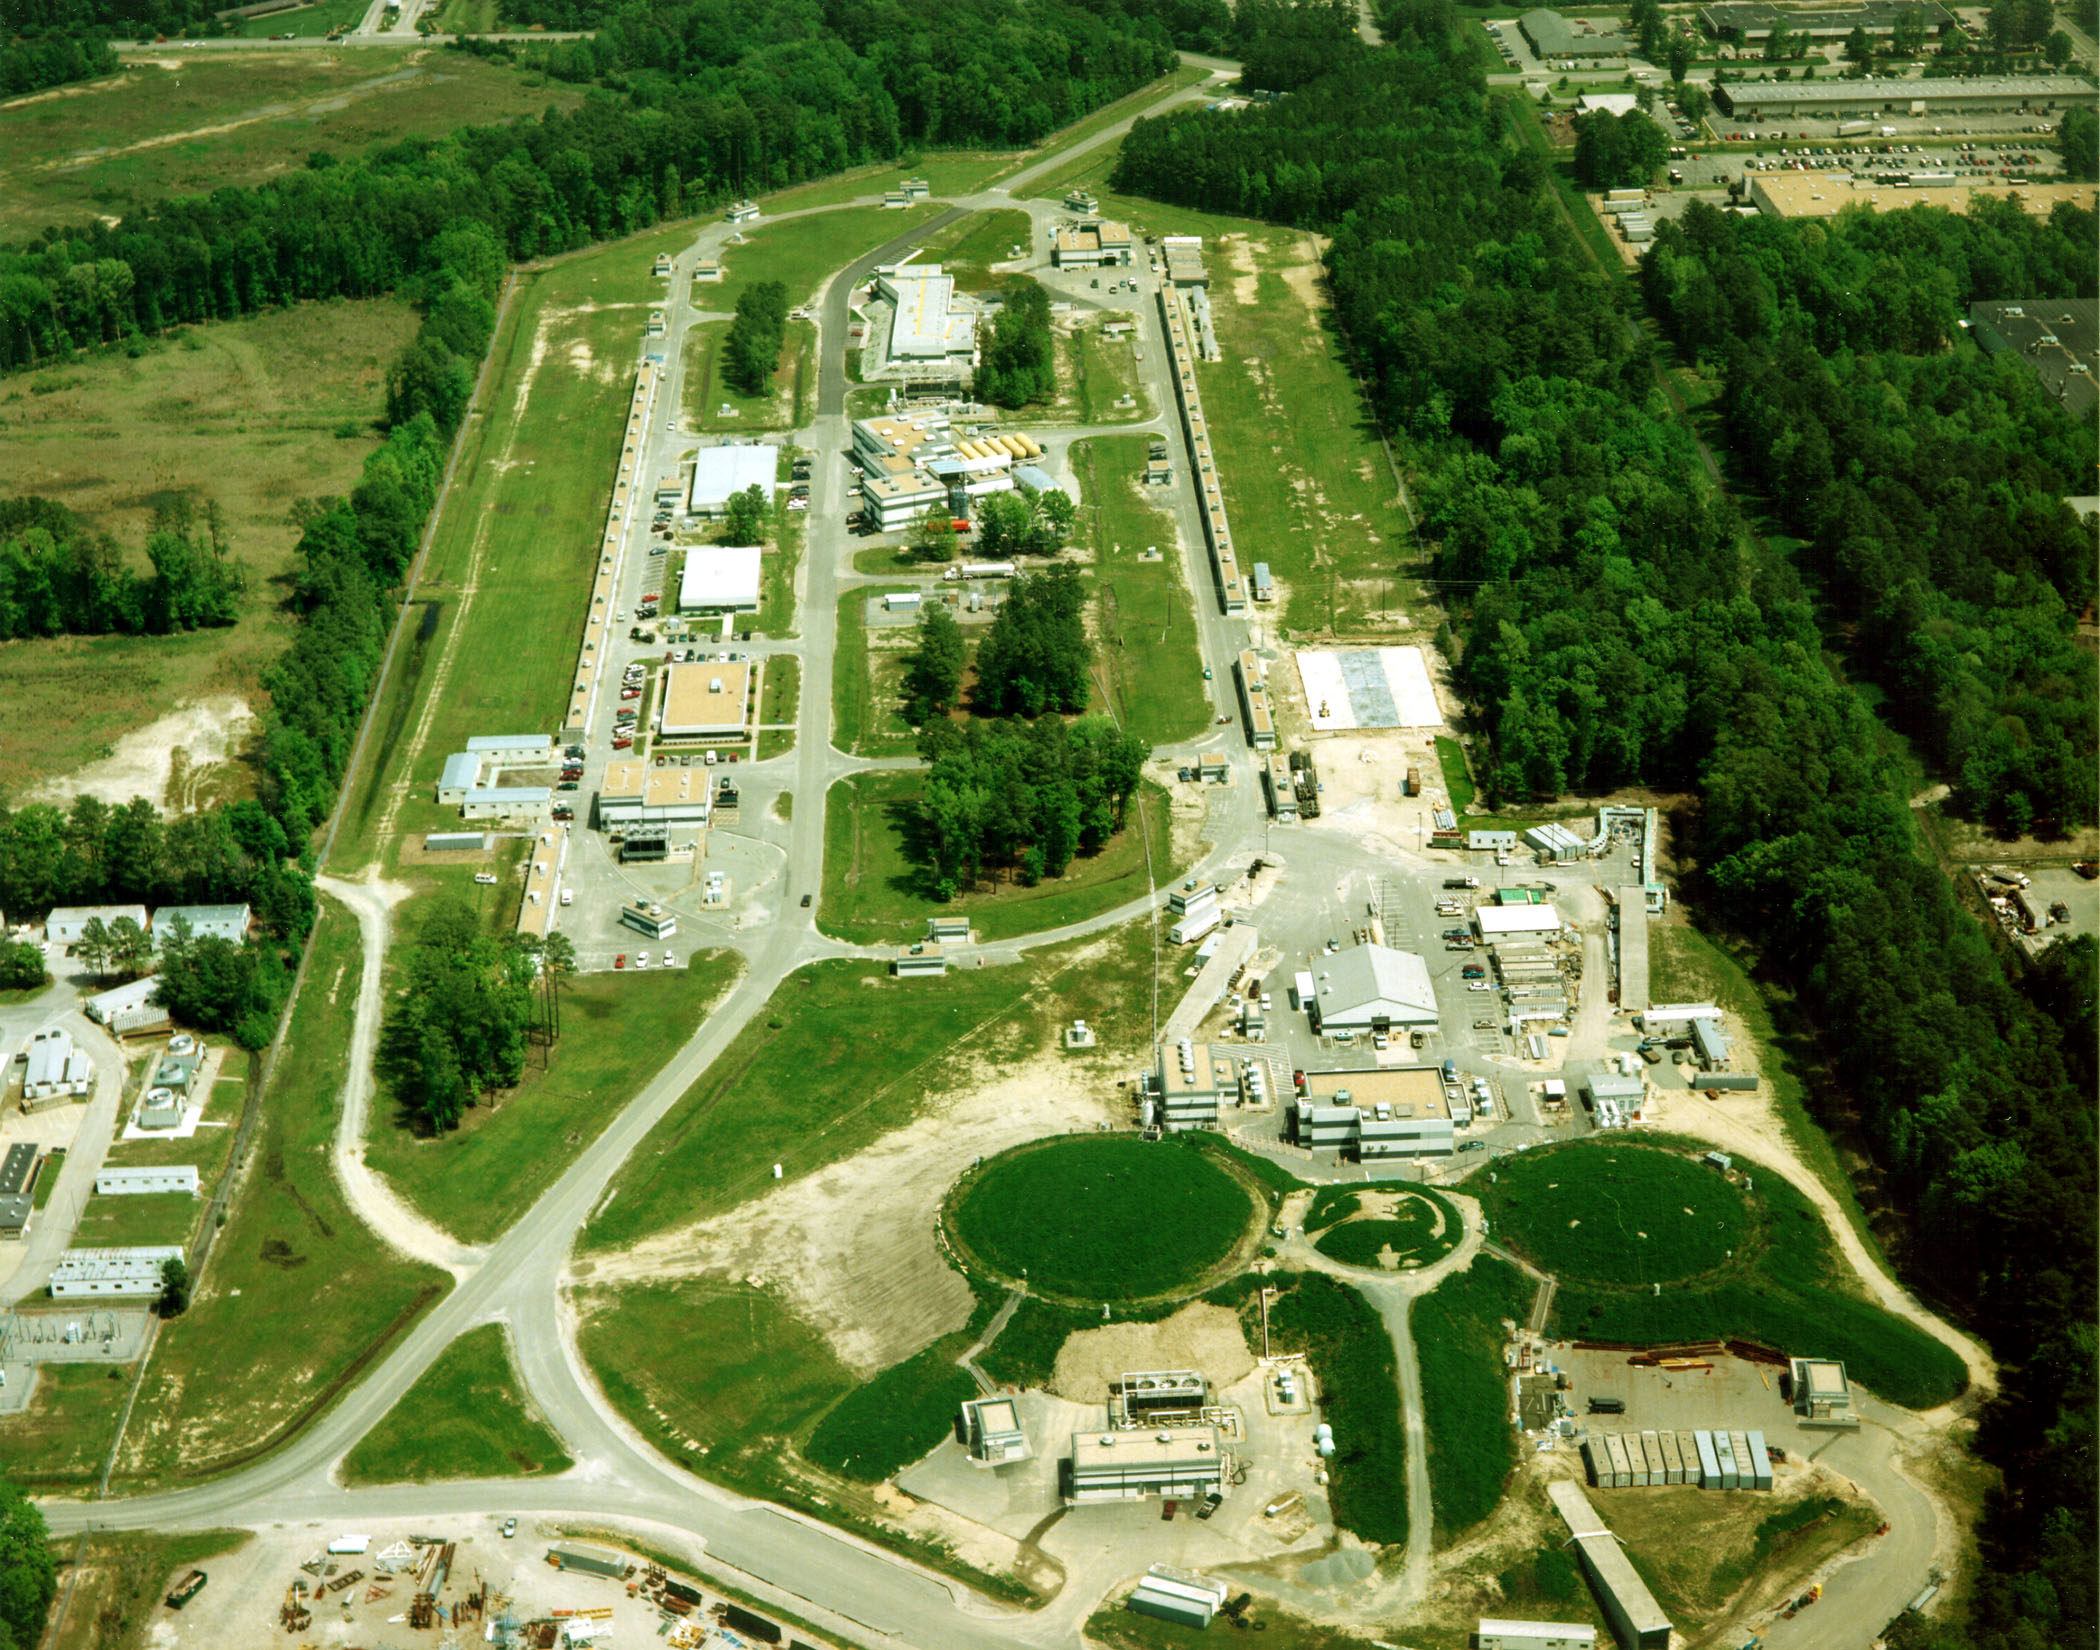
\includegraphics[width=.76349\textwidth]{Introduction/jlab.jpg}
                    
                    
                \end{figure}
                \vspace{-0.45cm}
            \begin{itemize}
                    \setlength\itemsep{1em}
                    \item Jefferson Lab aerial view
                    {\myfont{\tiny [jlab.org] }}
                    \end{itemize}
                    
            \column{0.5\textwidth}
                \begin{figure}[t!]
                    %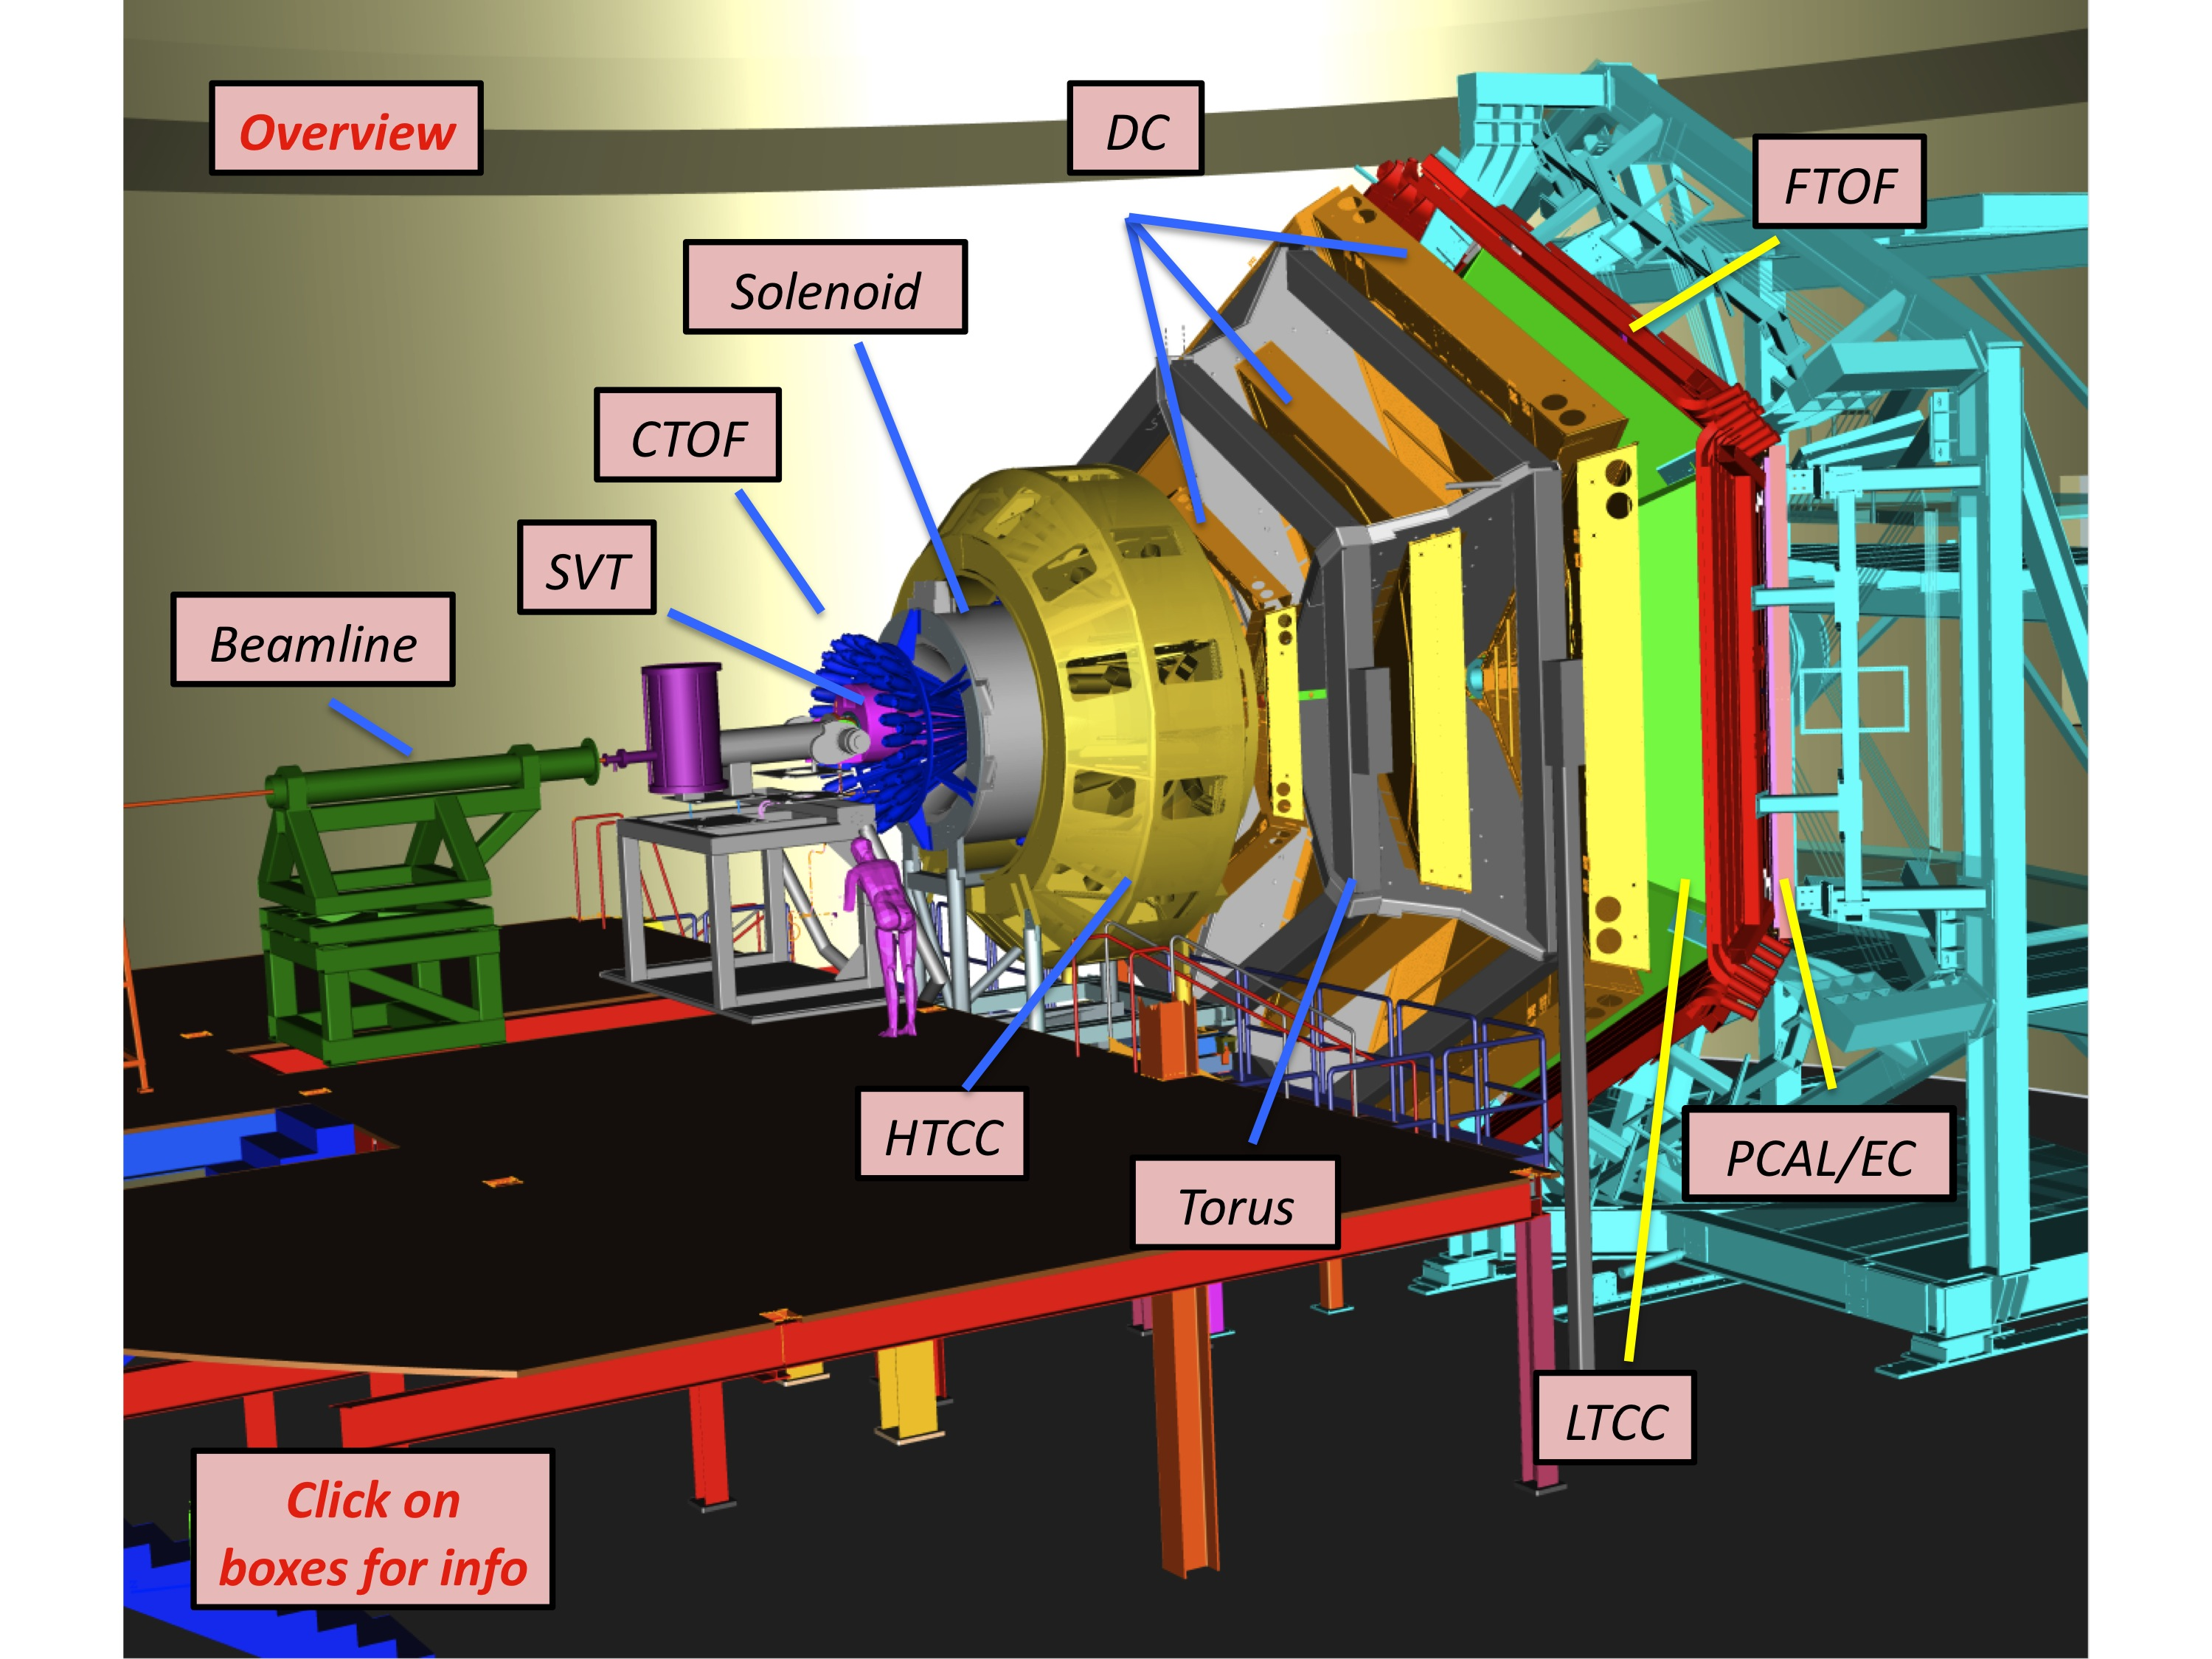
\includegraphics[height=\dimexpr0.5\textheight-0.5in]{Pics/dnp/clas12-overview.jpg}
                    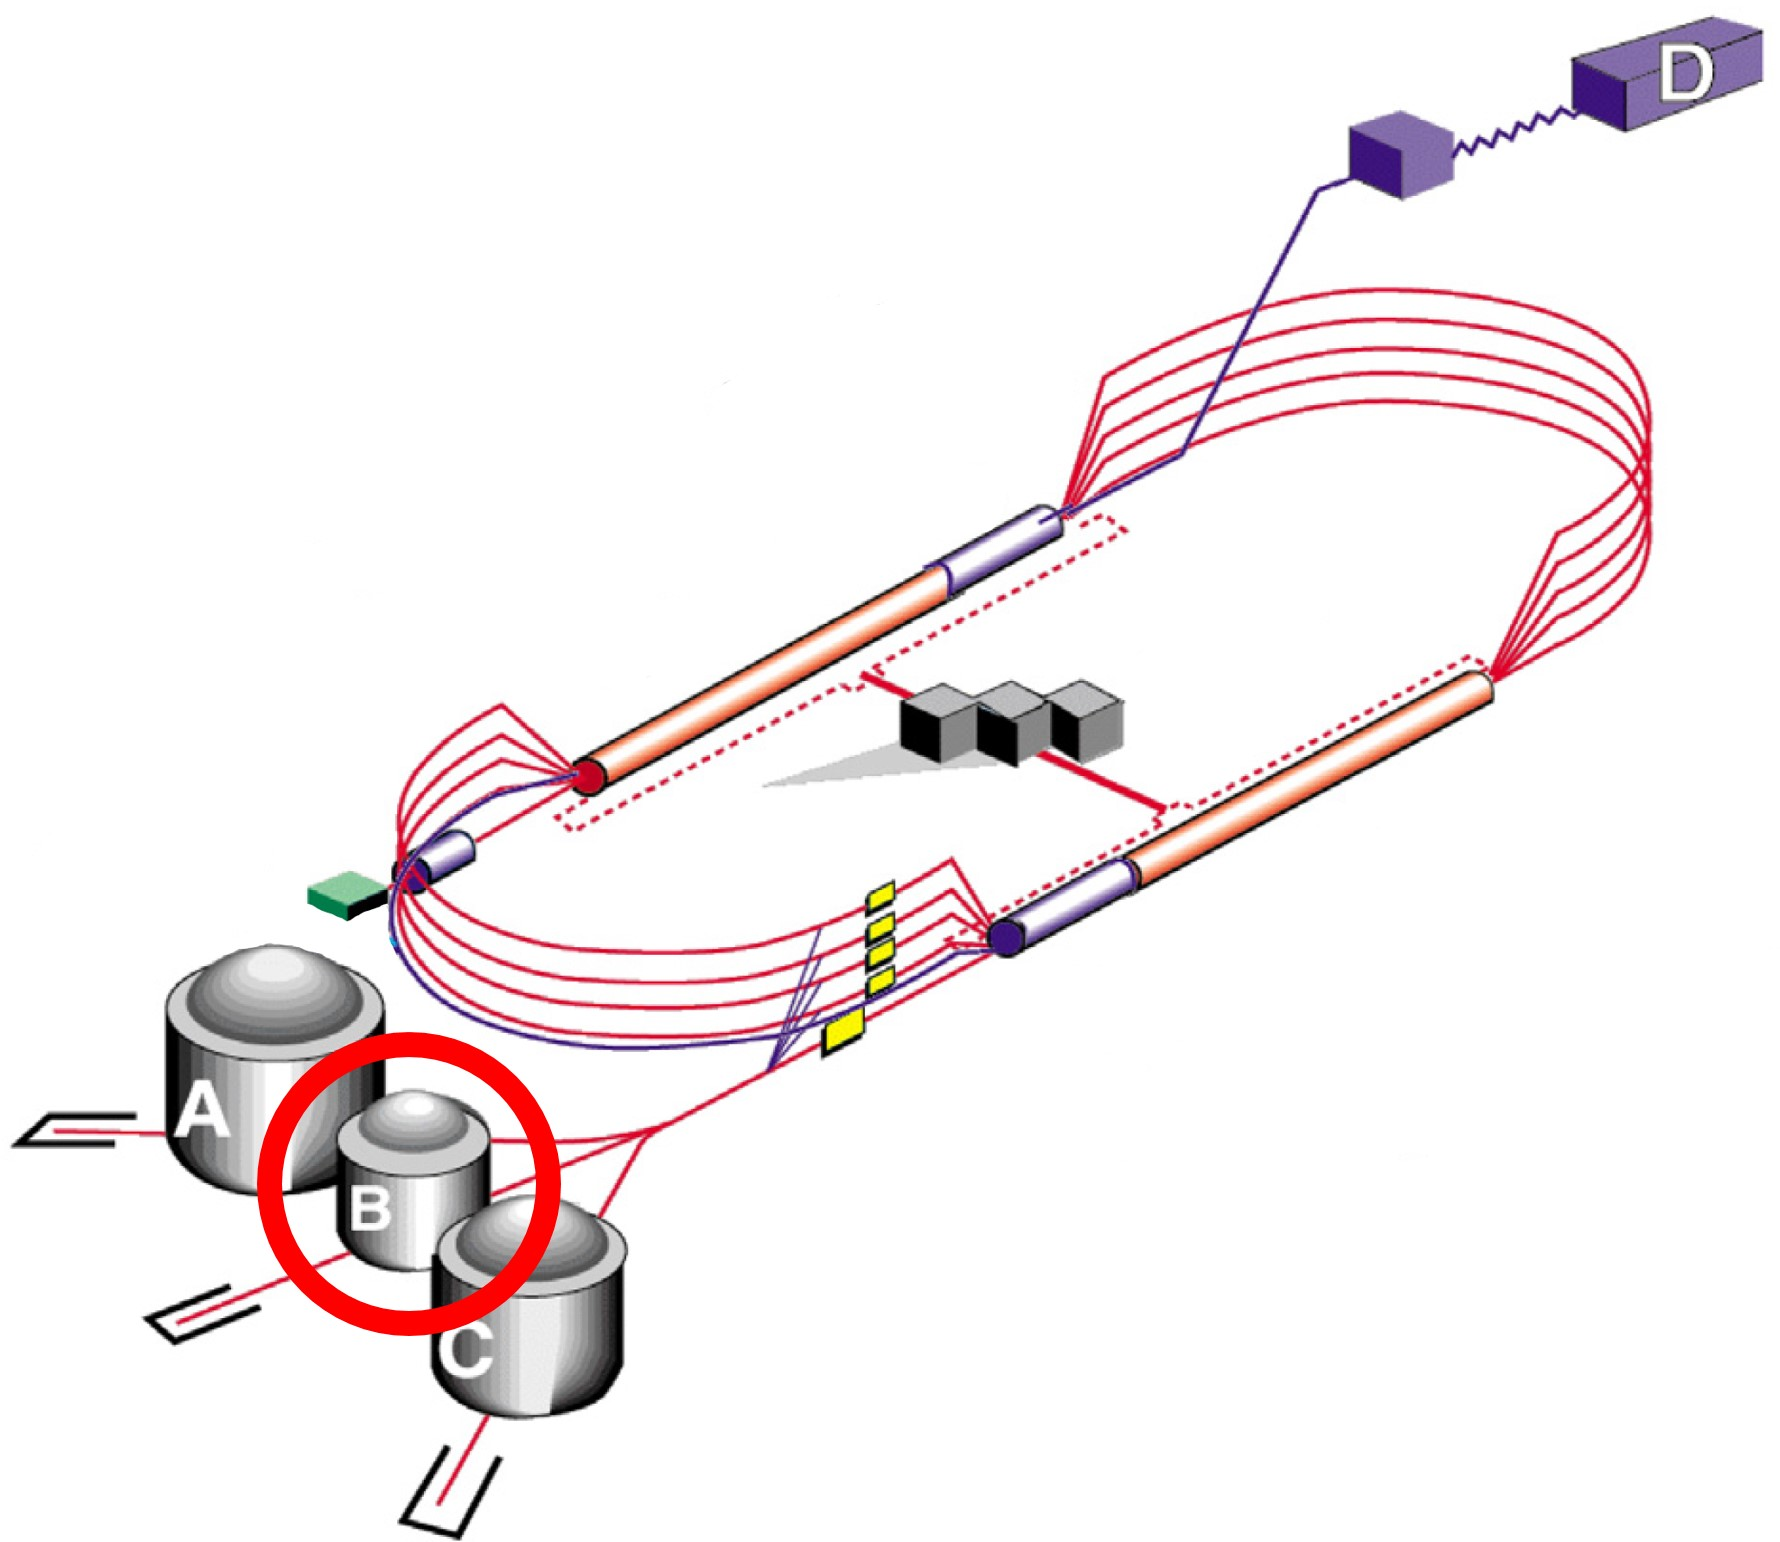
\includegraphics[width=.56765899\textwidth]{DNP/jlab_hall_b_circled.jpg}
                    
                    
                \end{figure}
                \vspace{-0.45cm}
                  \begin{itemize}
                    \setlength\itemsep{1em}
                    \item CEBAF 1,400 m racetrack, 50 RF cryomodules
                    \item 10.6 GeV, $\sim$ 50 nA electron beam
                    \end{itemize}
            
                \vspace{0.3cm}
                {\myfont{\tiny [V. Burkert et al., NIMA, 959, 163419 (2020)] }}
        \end{columns}
\end{frame}    


\begin{frame}{CLAS12 Detector at Jefferson Lab Hall B} \label{frame:datasets2}
        \vspace{-0.5cm}
        \begin{columns}[t, onlytextwidth]
            \column{0.5\textwidth}
                %\vspace{1cm}
                \begin{figure}[t!]
                    %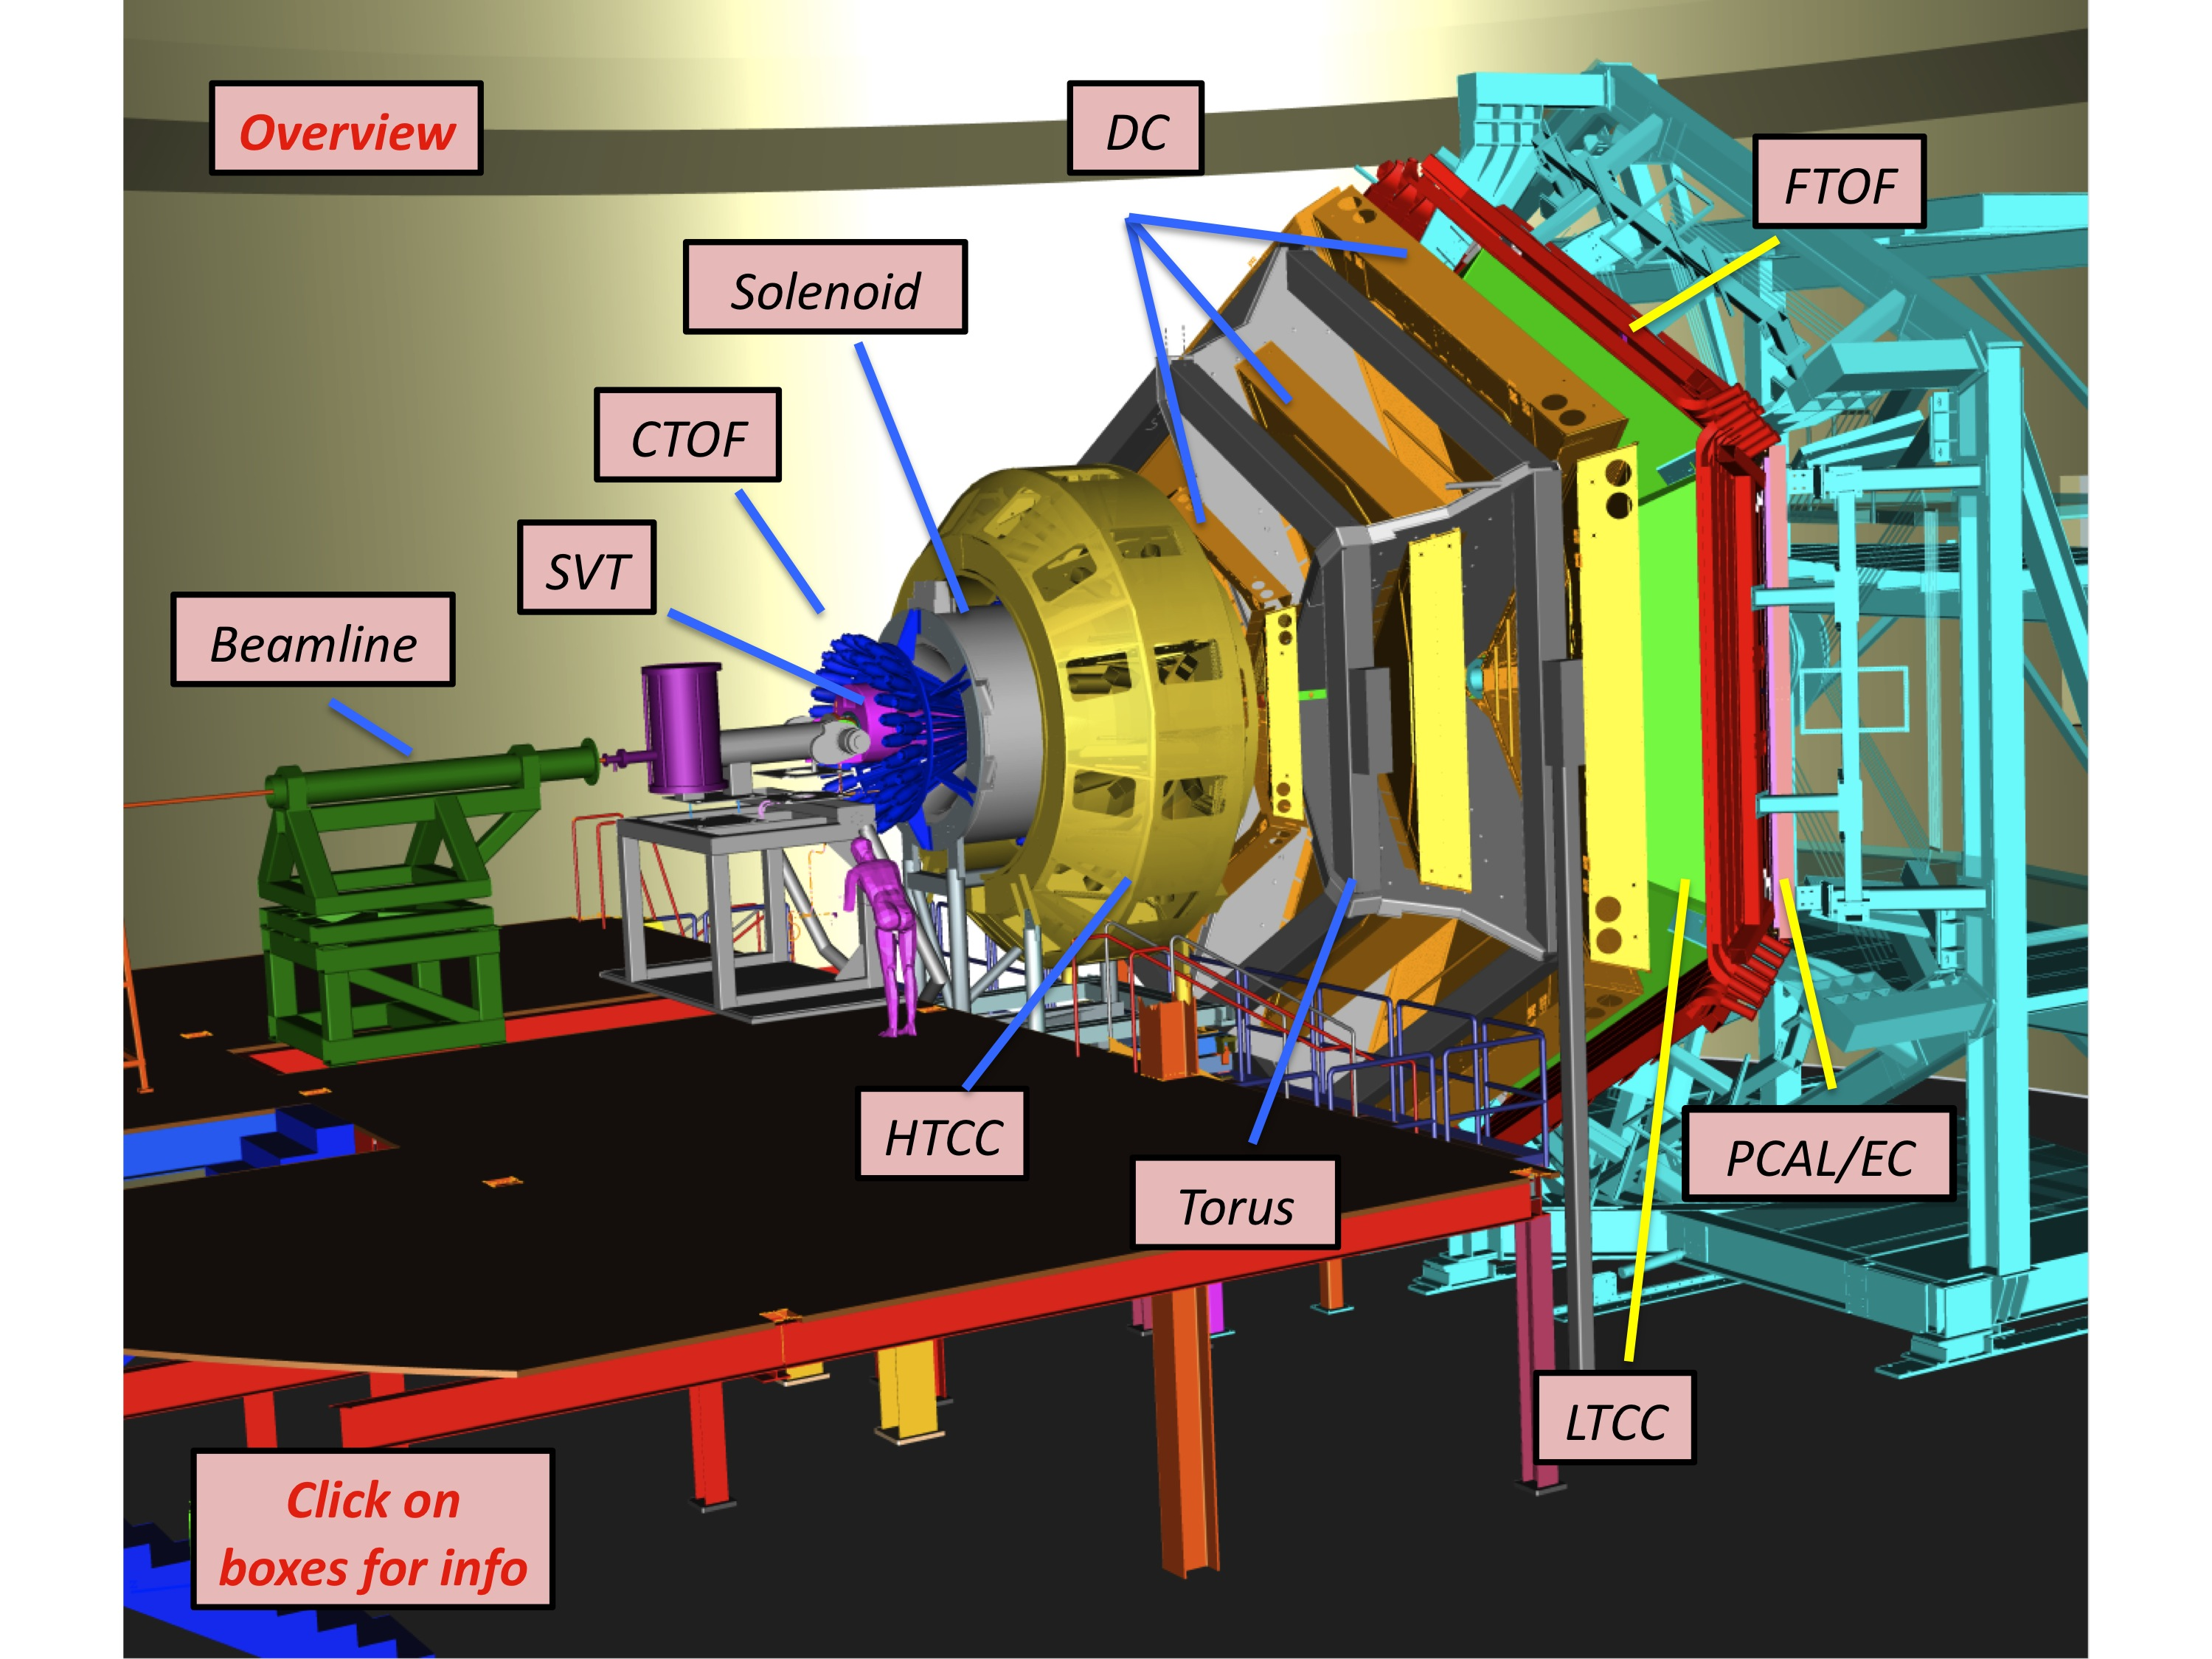
\includegraphics[height=\dimexpr0.5\textheight-0.5in]{Pics/dnp/clas12-overview.jpg}
                    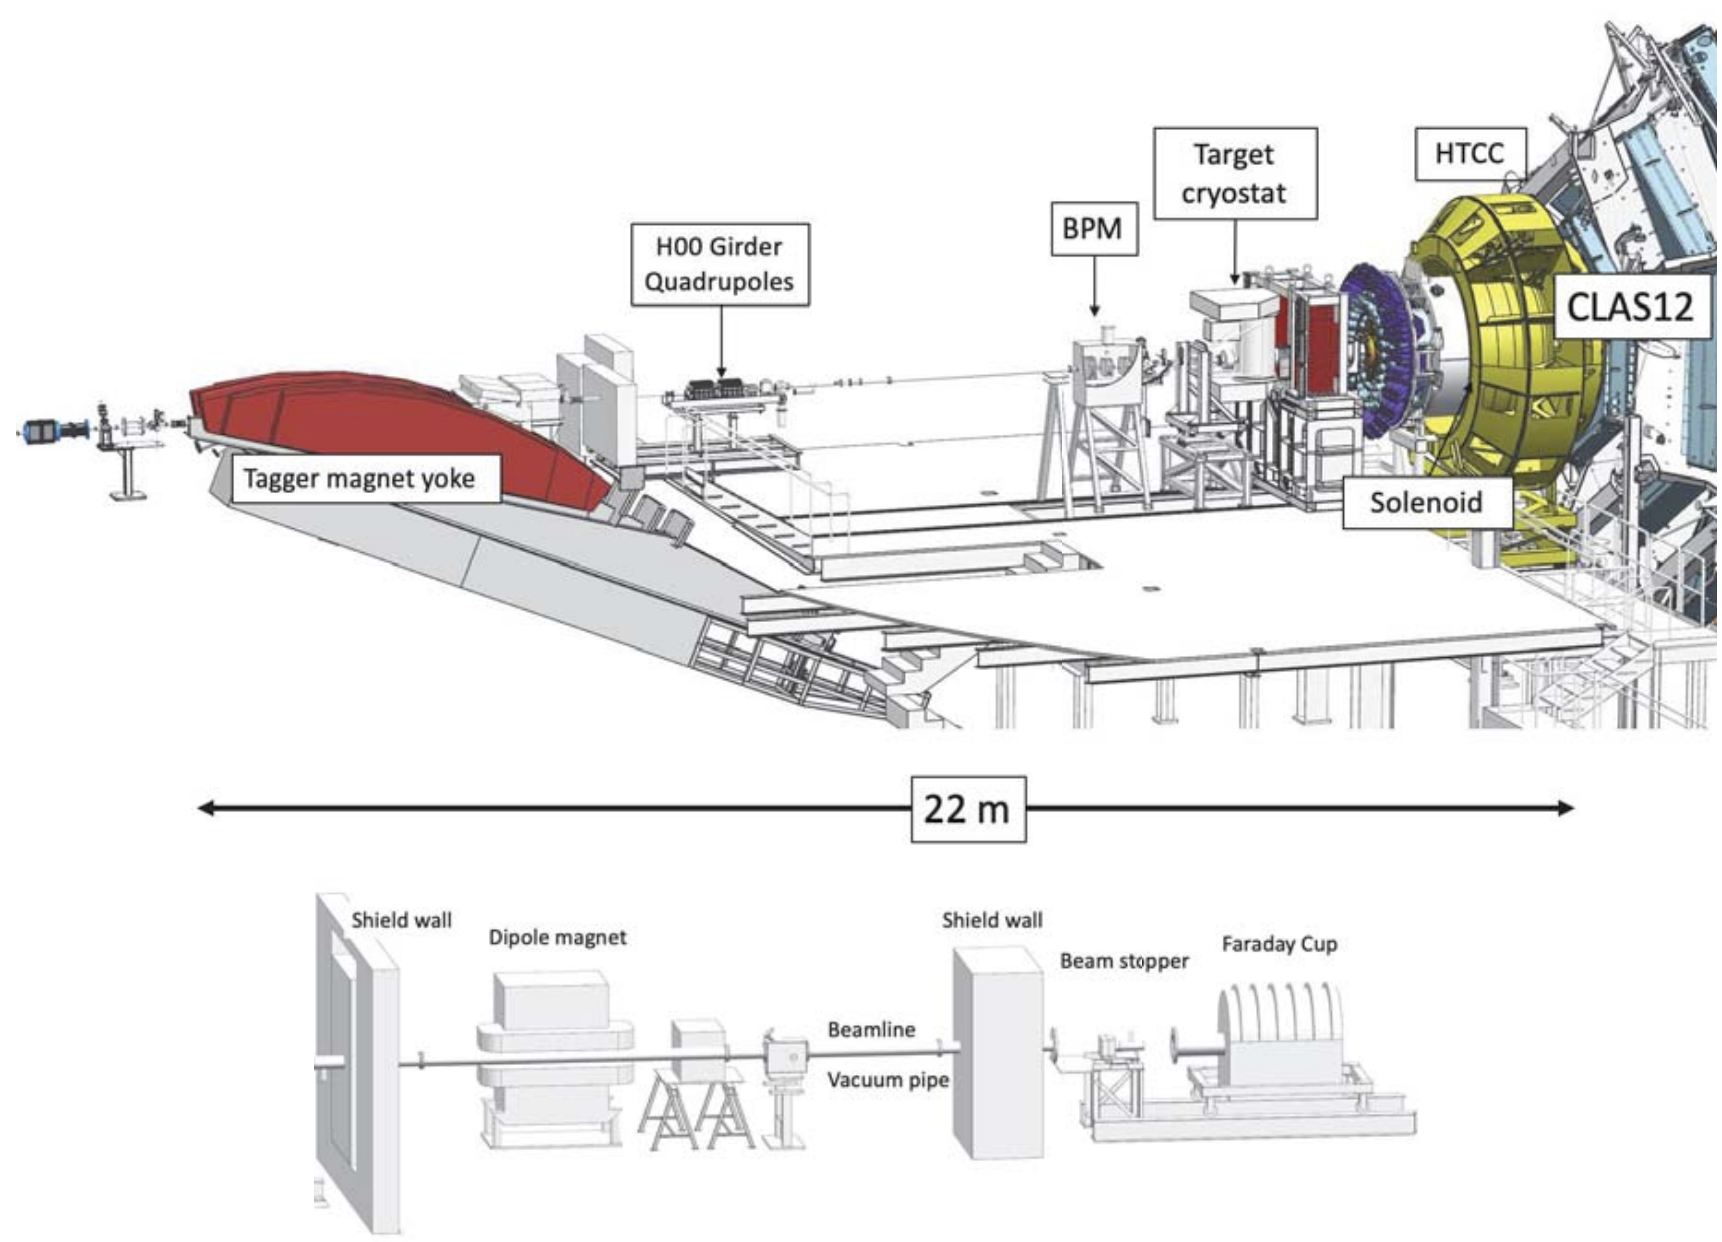
\includegraphics[width=.86349\textwidth]{Main/beamline.png}
                    
                    
                \end{figure}
                \vspace{-0.45cm}
                  \begin{itemize}
                    \setlength\itemsep{1em}
                    \item  Top: Beamline into unpolarized LH$_2$ target (cryostat)
                    \item Bottom: Downstream beamline to Faraday Cup (current monitor)
                    \end{itemize}
                    
            \column{0.5\textwidth}
                \begin{figure}[t!]
                    %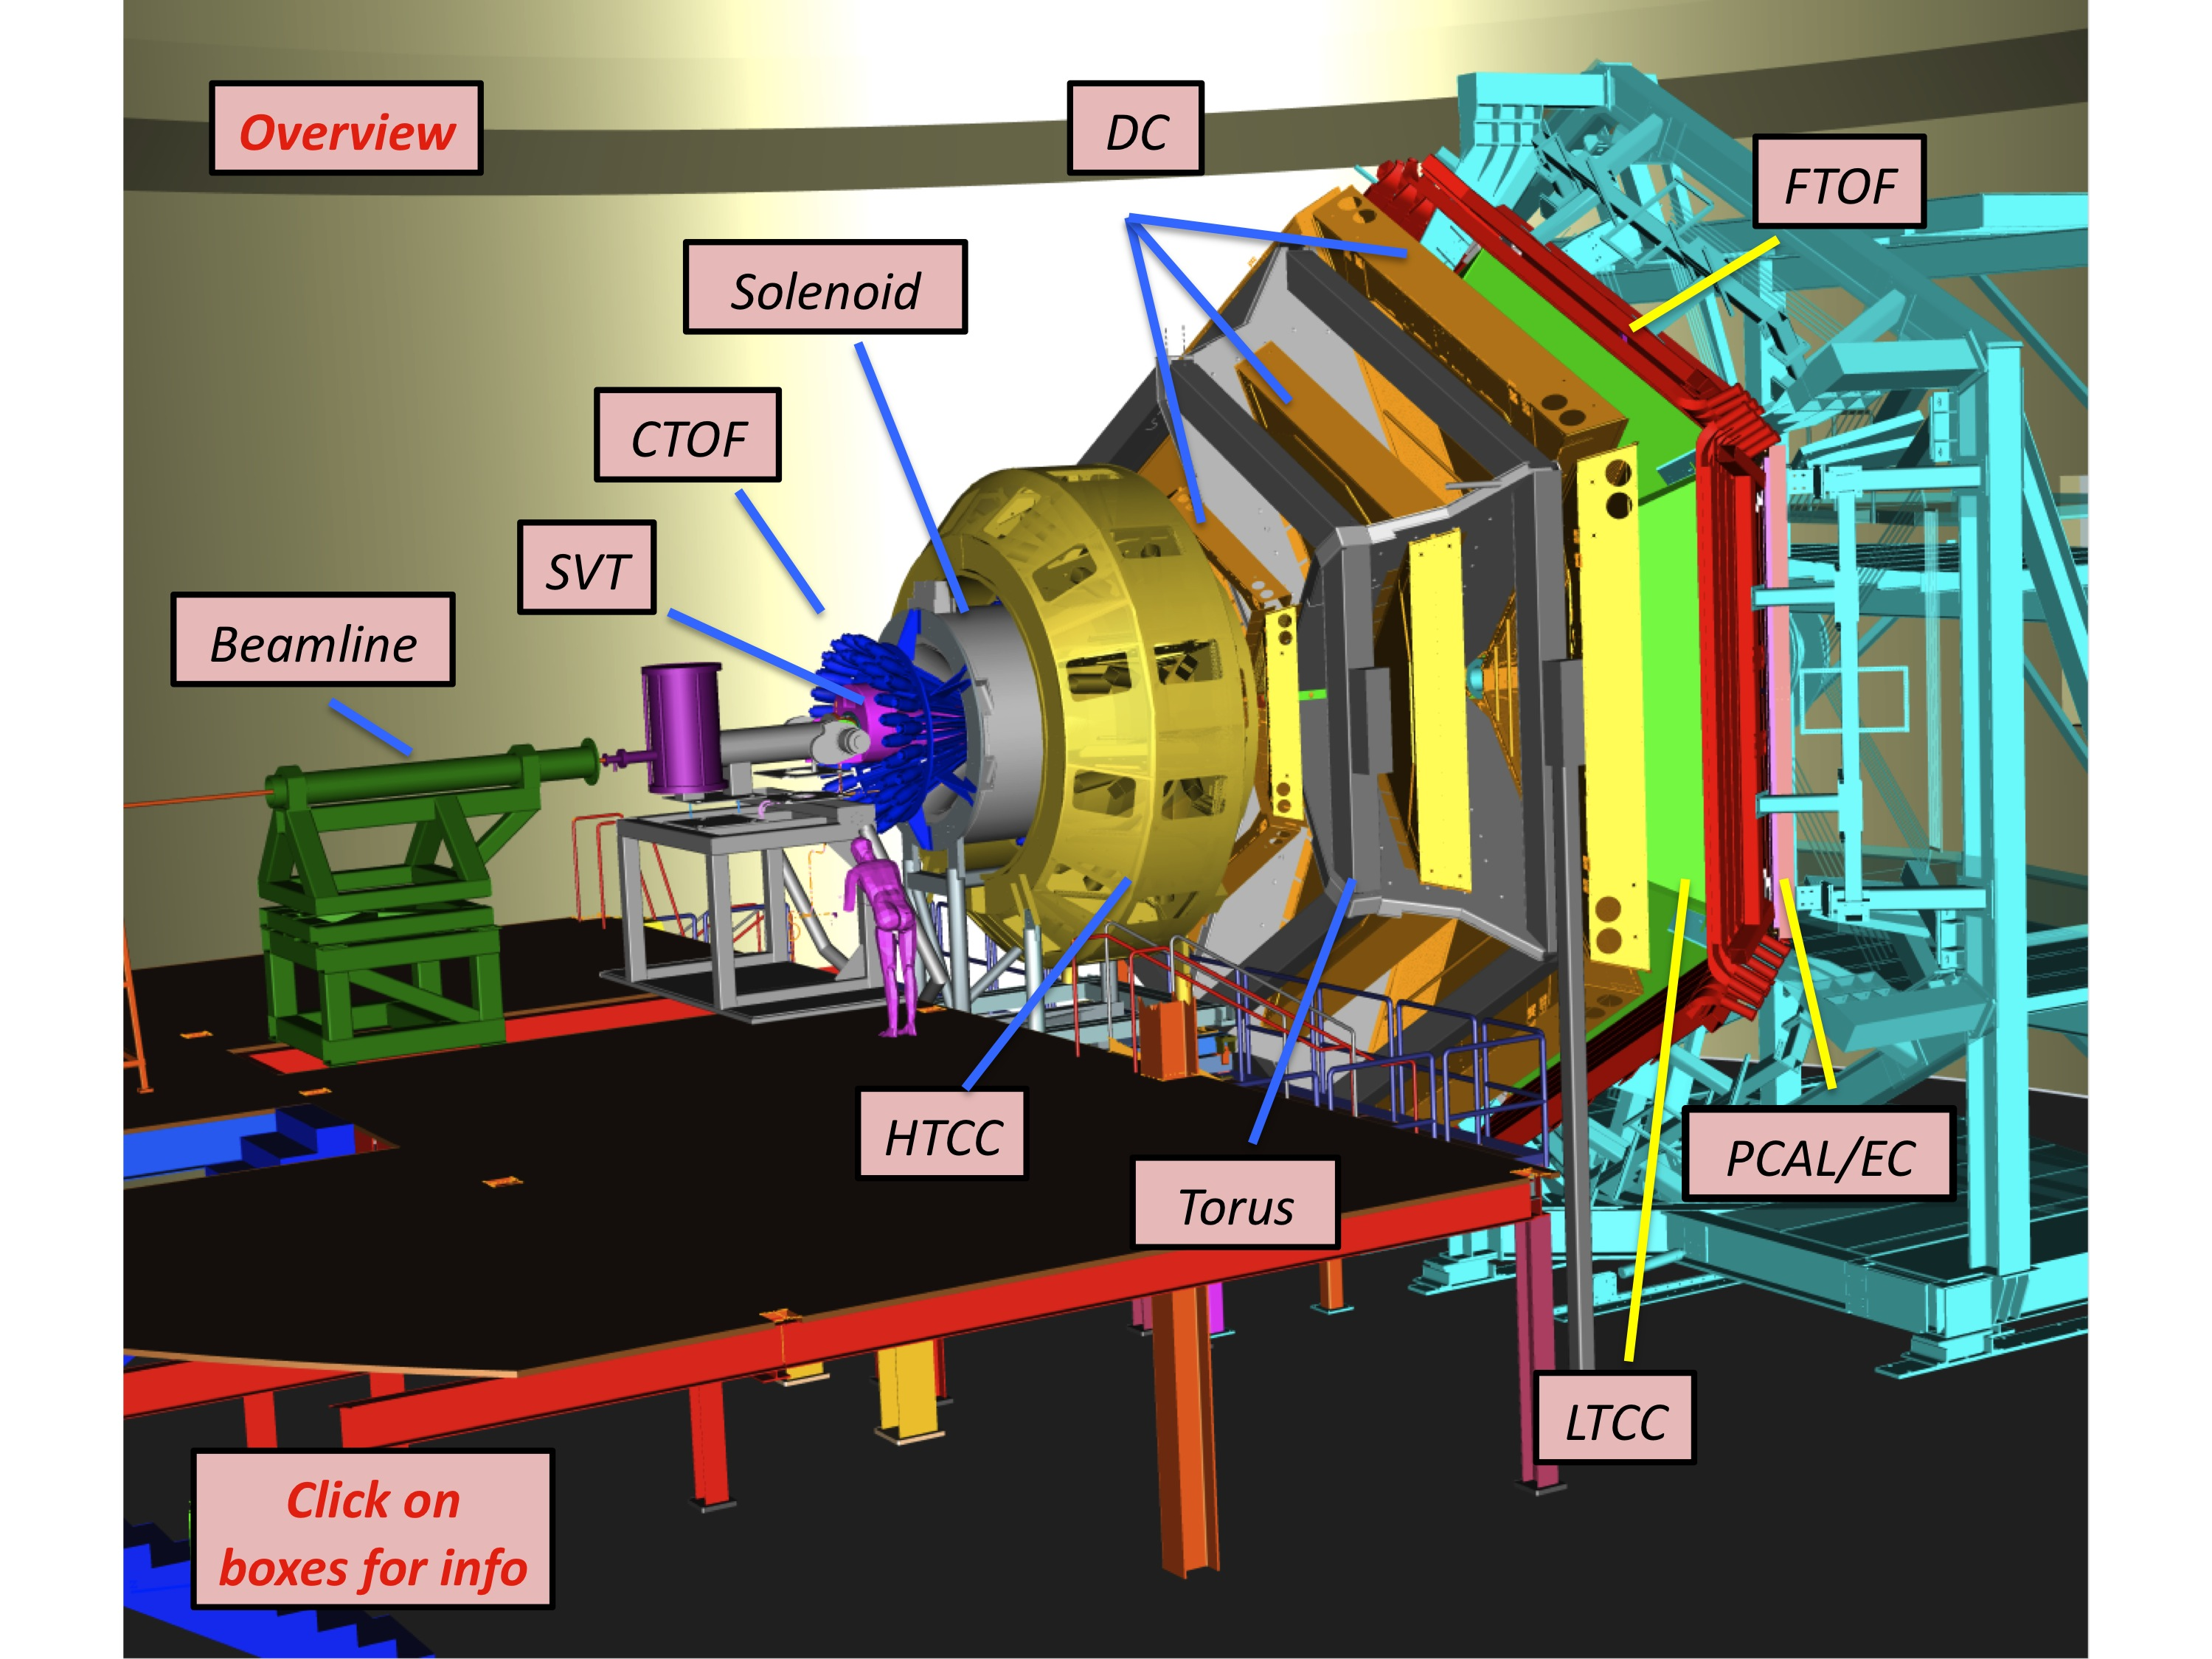
\includegraphics[height=\dimexpr0.5\textheight-0.5in]{Pics/dnp/clas12-overview.jpg}
                    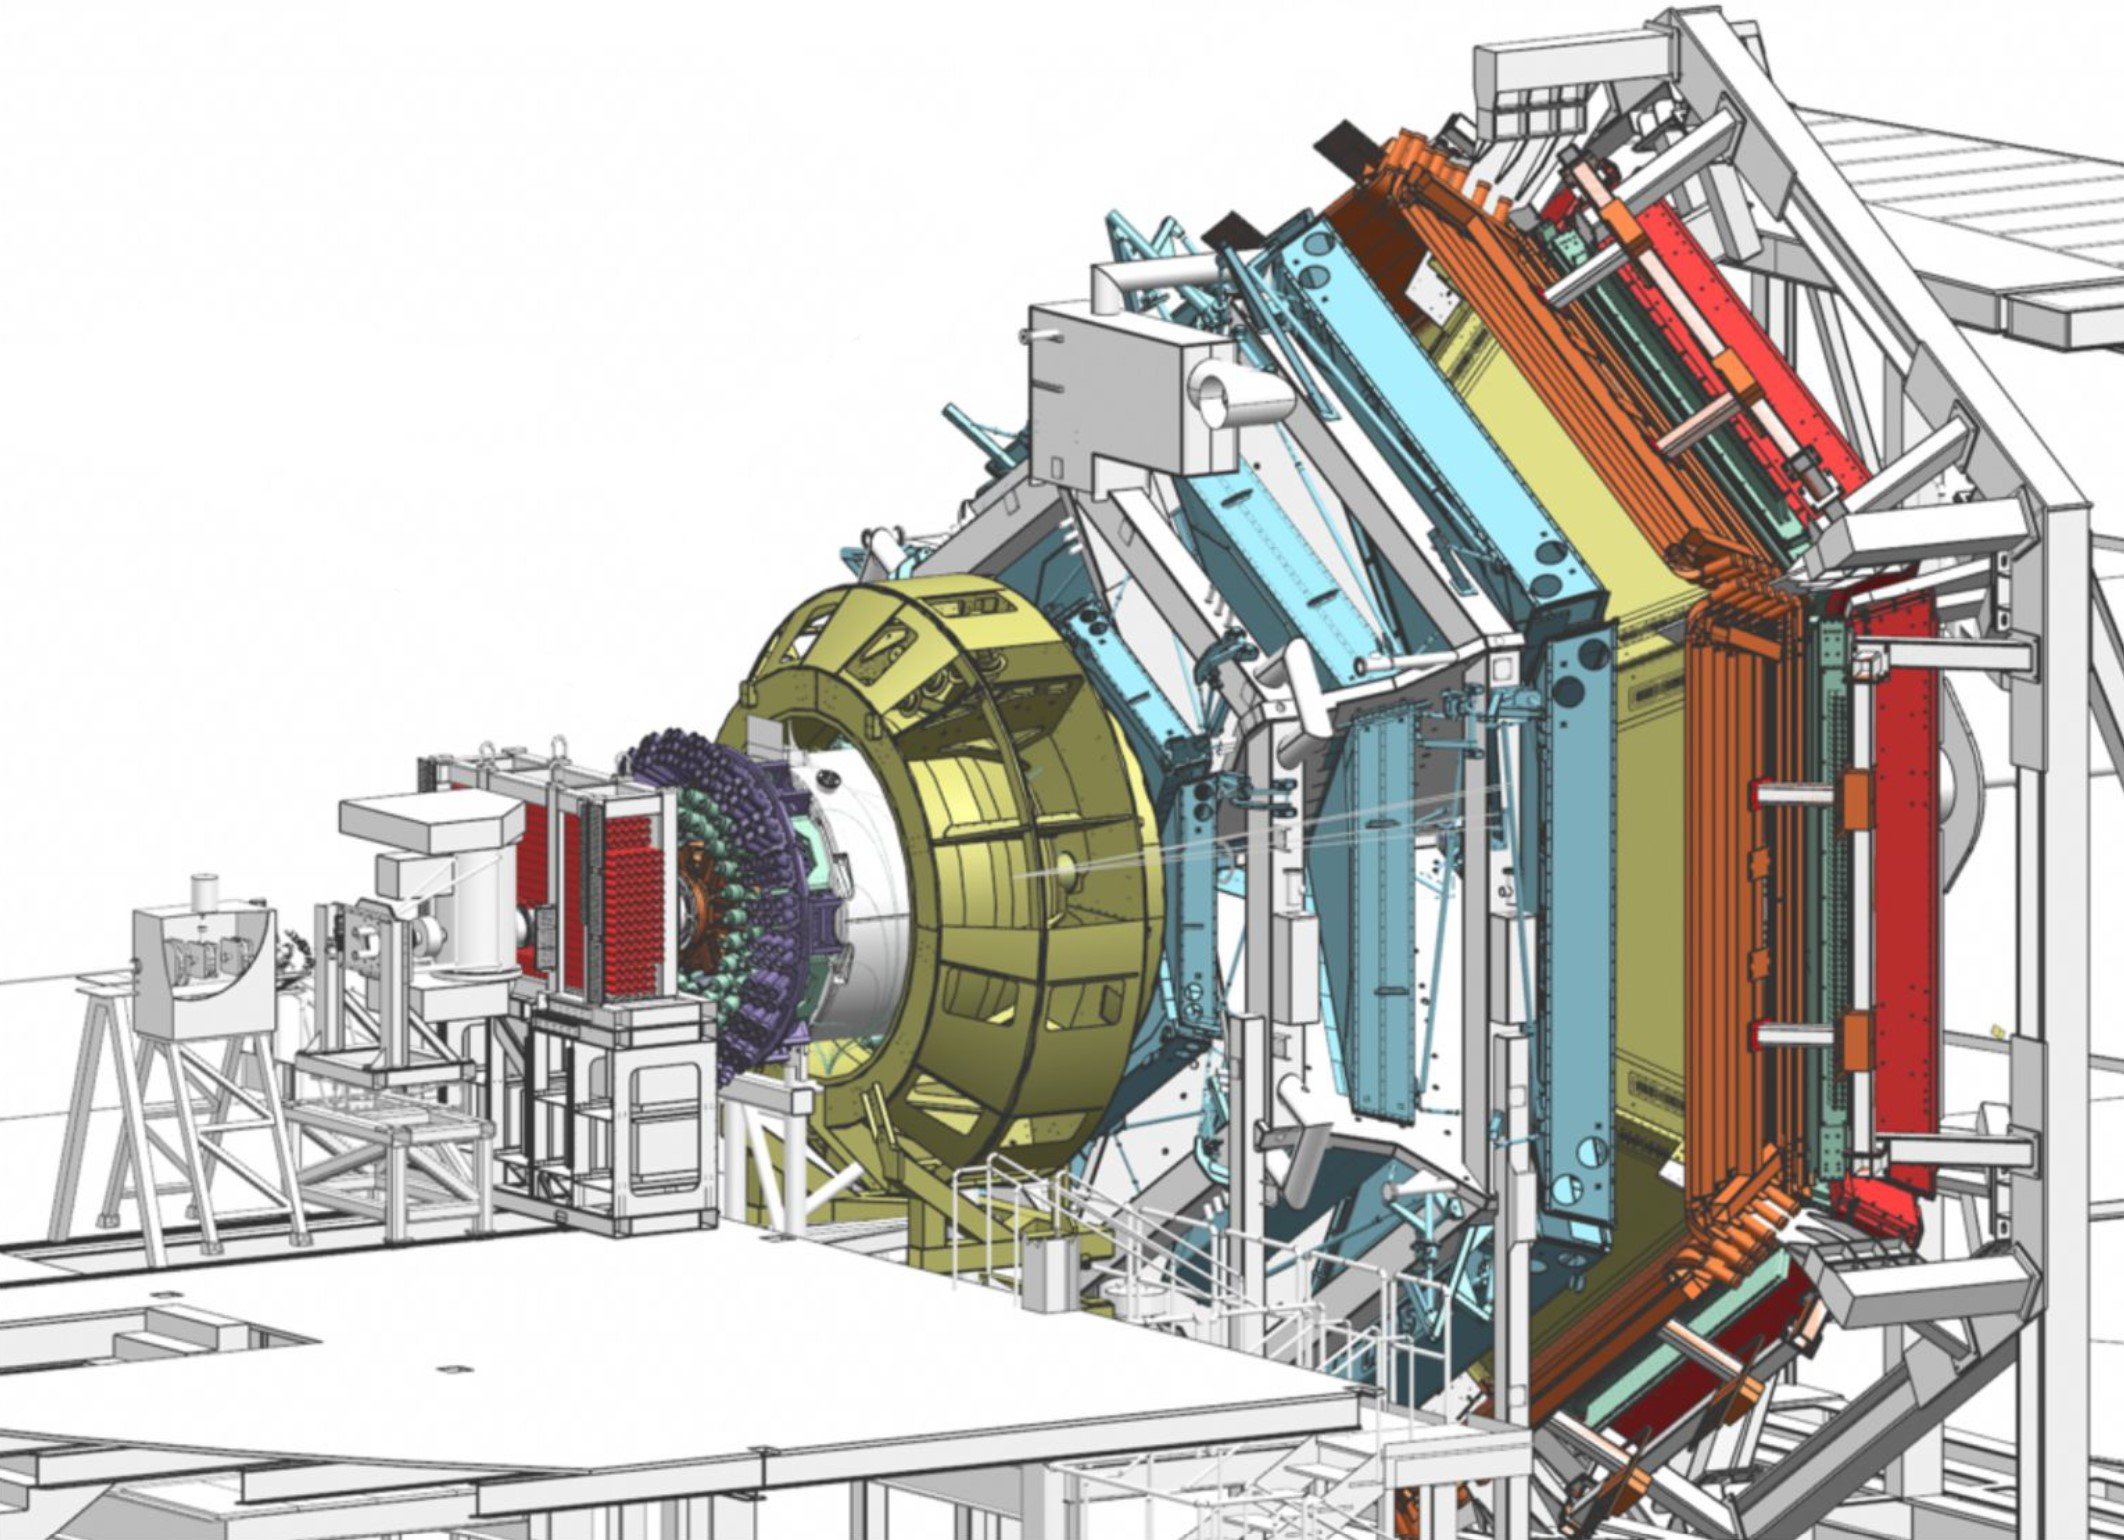
\includegraphics[width=.8565899\textwidth]{DNP/CLASdetector.jpg}
                    
                    
                \end{figure}
                \vspace{-0.45cm}
                \begin{itemize}
                    \setlength\itemsep{1em}

                    \item CEBAF Large Acceptance Spectrometer:\\
                     \begin{itemize}
                            \item $\sim$ 2$\pi$ coverage in $\phi$\\
                        \item  $5^\circ$ - $125^\circ$ coverage in $\theta$
                        \item Full 4 particle final state reconstruction for this process
                    \end{itemize}
                    
                    
                \end{itemize}
                %\vspace{0.3cm}
                {\myfont{\tiny [V. Burkert et al., NIMA, 959, 163419 (2020)] }}
        \end{columns}
\end{frame}    


\begin{frame}{Experiment Layout And Particle Detection} \label{frame:datasets3}
\vspace{-0.5cm}
        \begin{columns}[t, onlytextwidth]
            \column{0.55\textwidth}
                \begin{itemize}
                    \setlength\itemsep{.35em}
                    \item 6-fold symmetric Forward Detector ($\theta < \sim 40 ^{\circ}$) with torodial field
                     \begin{itemize}
                    \setlength\itemsep{.25em}
                        \item Cherenkov Counters
                        \item Drift Chambers
                        \item Time-of-Flight Detectors
                        \item EM Calorimeters
                    \end{itemize}
                      \item Central Detector ($\sim40 < \theta < \sim 125 ^{\circ}$) \\
                      inside solenoid
                     \begin{itemize}
                    \setlength\itemsep{.25em}
                        \item Silicon Vertex Tracker
                        \item Micromegas
                        \item ToF Detector

                    \end{itemize}
                    
                    \item Forward Tagger, Backward Angle Neutron Detector
                    \item Faraday Cup for luminosity measurement
                
            
                \end{itemize}
            
                \vspace{0.1cm}
                
            \column{0.45\textwidth}
                %\vspace{1cm}
                \vspace{0.3cm}
                \begin{figure}[t!]
                    %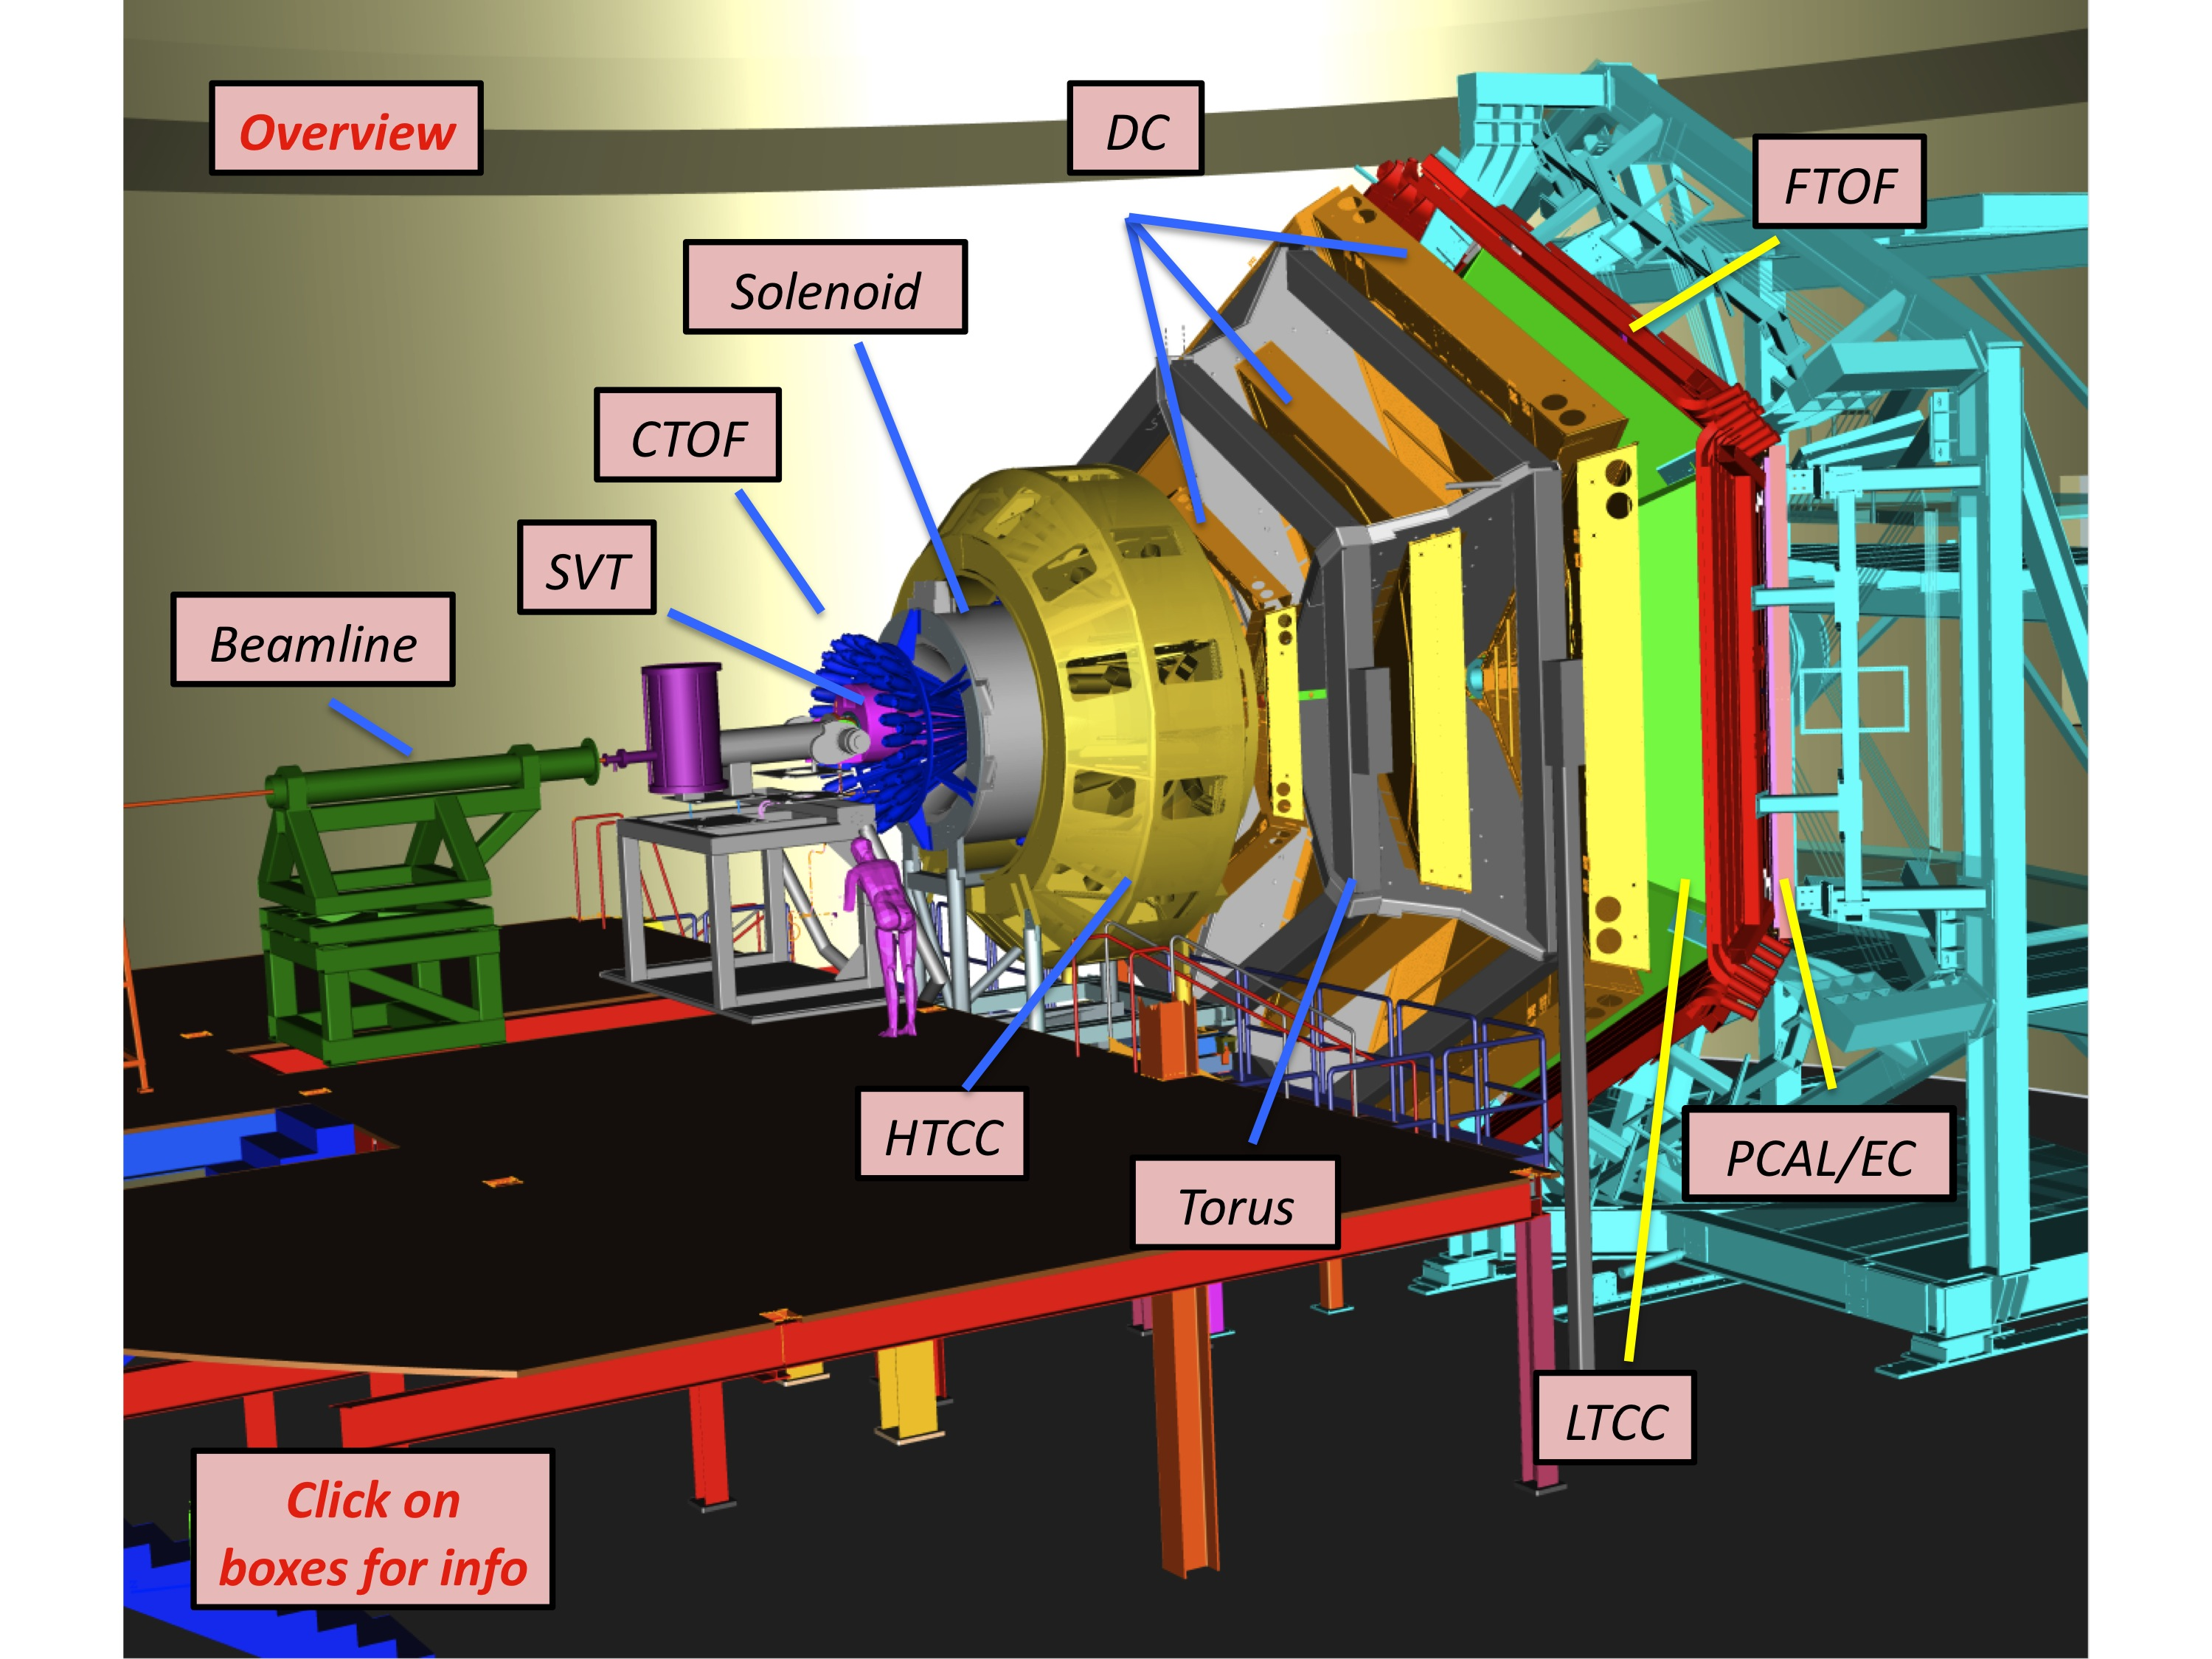
\includegraphics[height=\dimexpr0.5\textheight-0.5in]{Pics/dnp/clas12-overview.jpg}
                    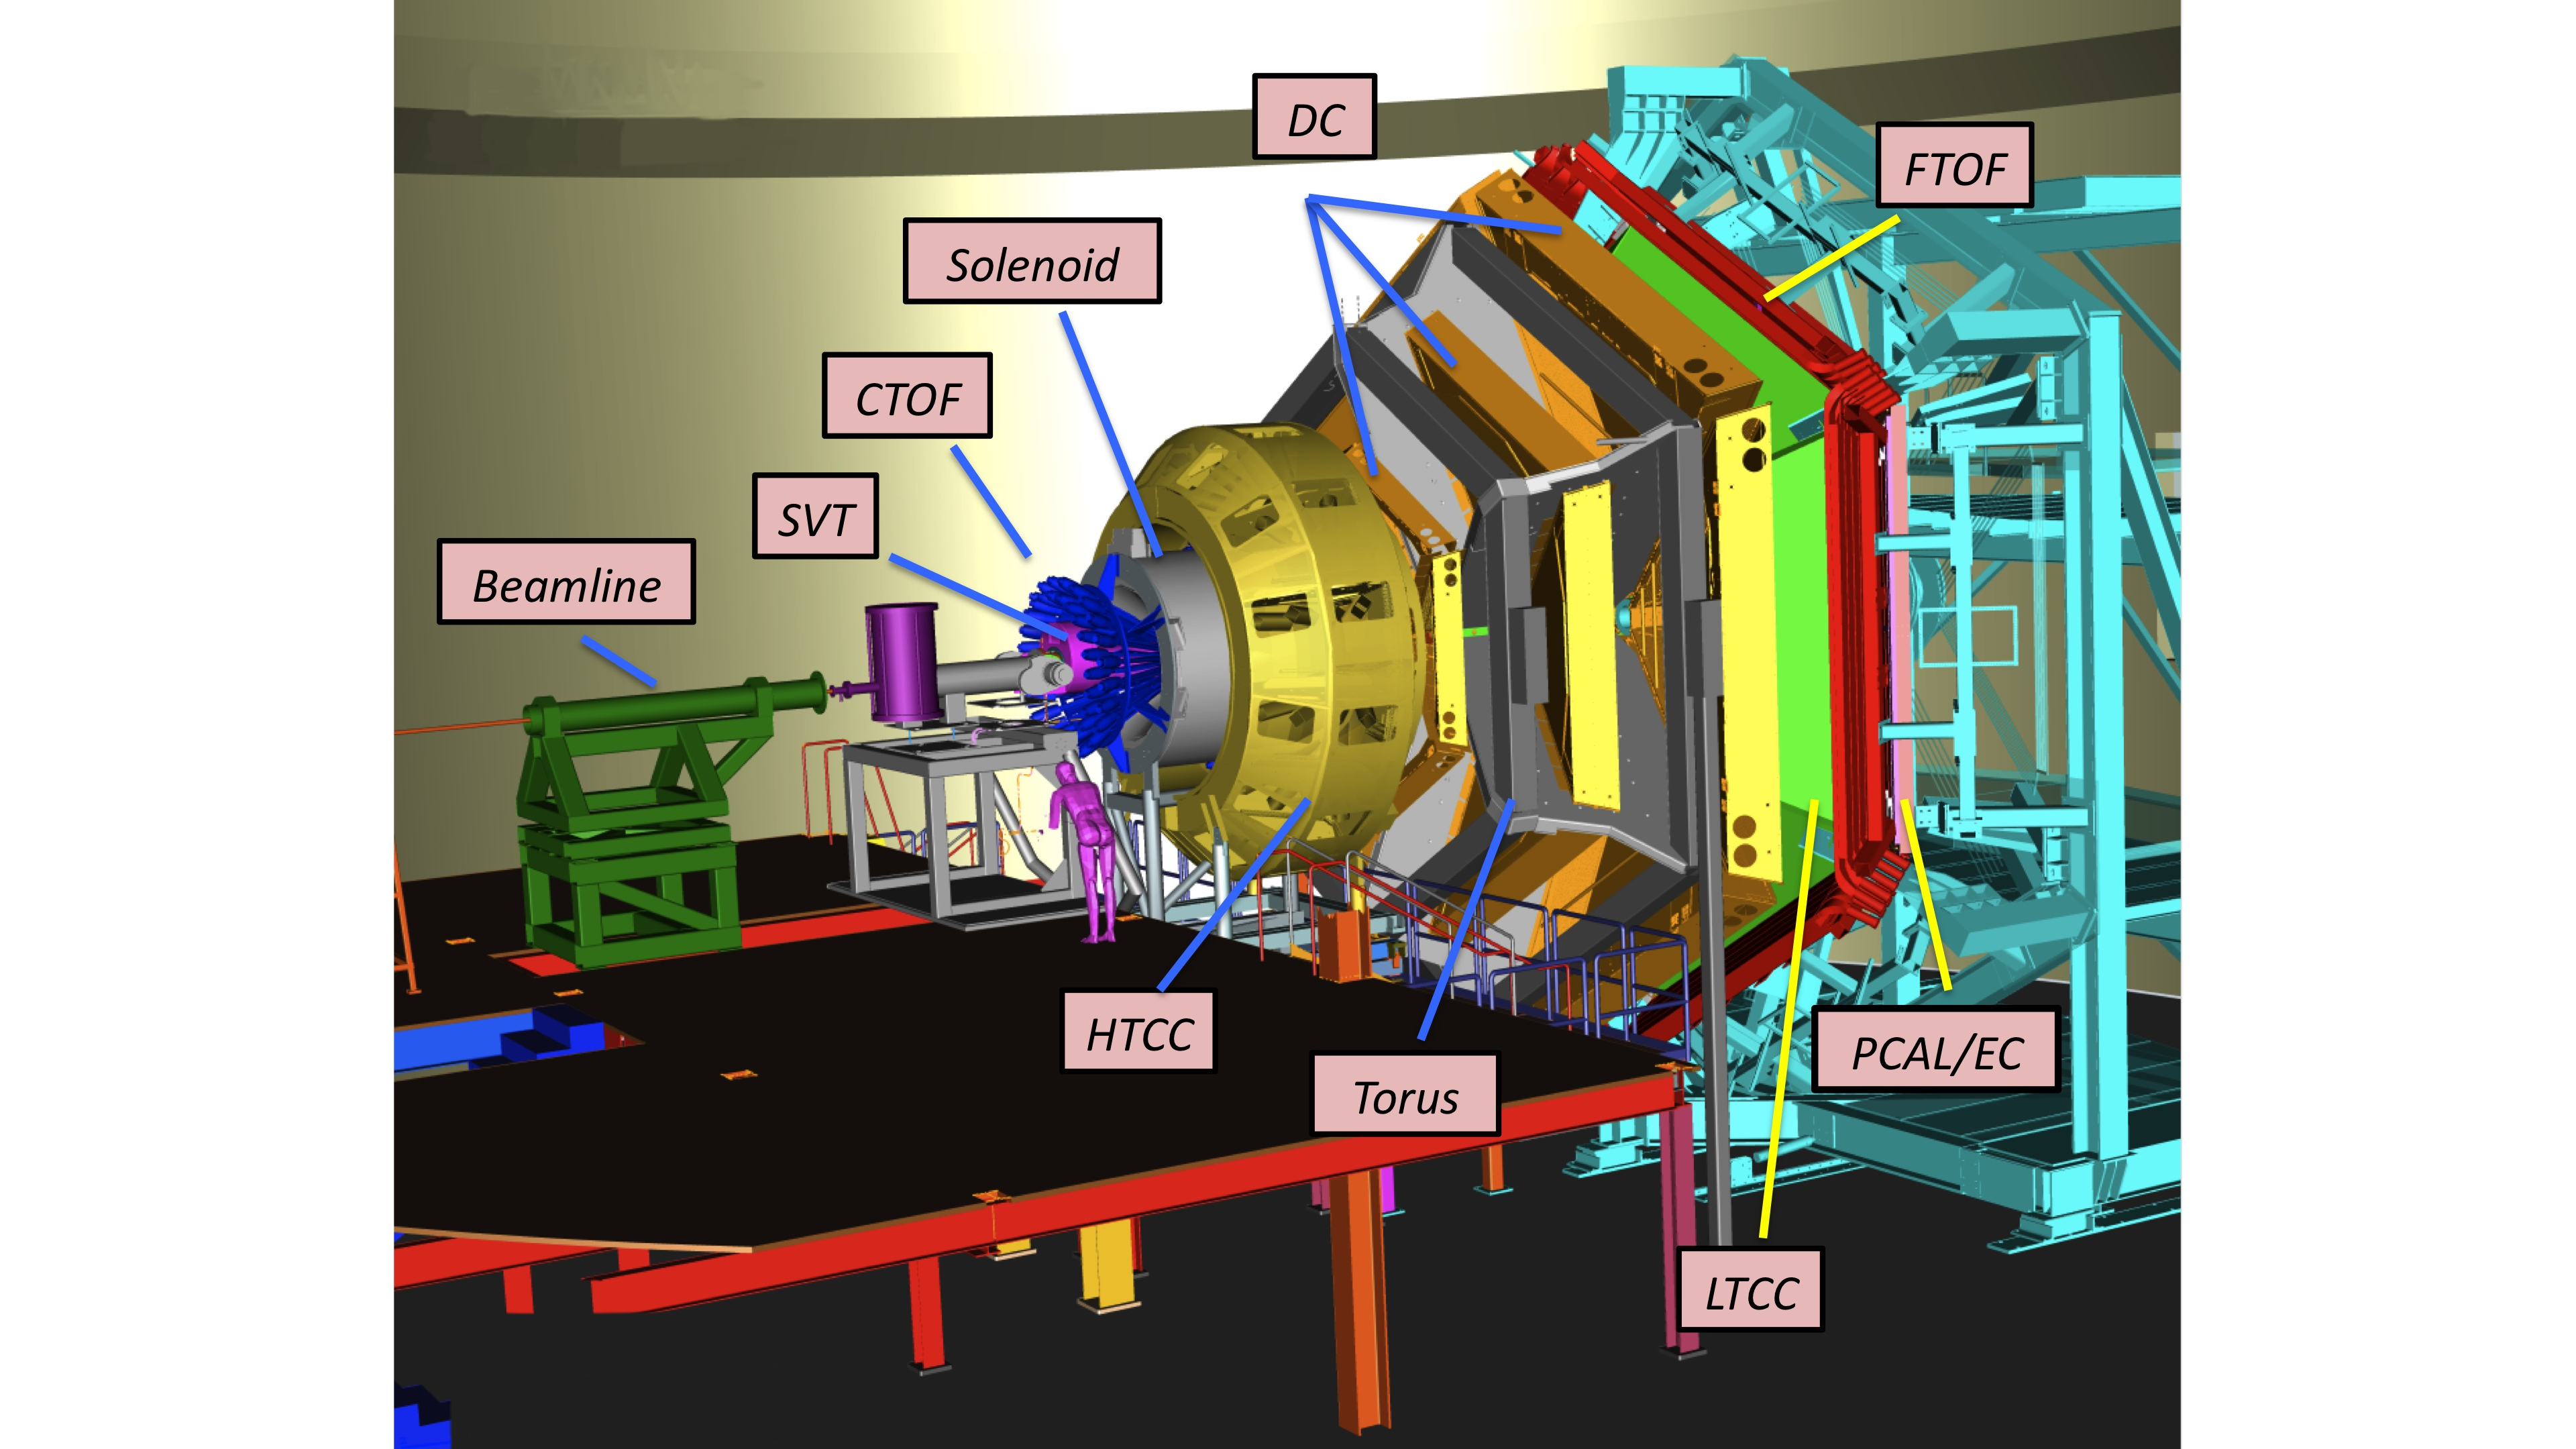
\includegraphics[trim={8cm 1cm  8cm 1cm},width=.899\textwidth]{DNP/jlab_clas_layout_1.png}
                    

                    
                \end{figure}
                \begin{itemize}
                    \setlength\itemsep{.35em}
                    \item This analysis examines data taken in Fall 2018
                    \end{itemize}
                {\myfont{\tiny [V. Burkert et al., NIMA, 959, 163419 (2020)] }}
        \end{columns}
\end{frame}    


\begin{frame}{Analysis Overview: Components of Cross Section}

                %\textcolor{white}{blank space}
                \centering 
                %#---------------------------------------------
                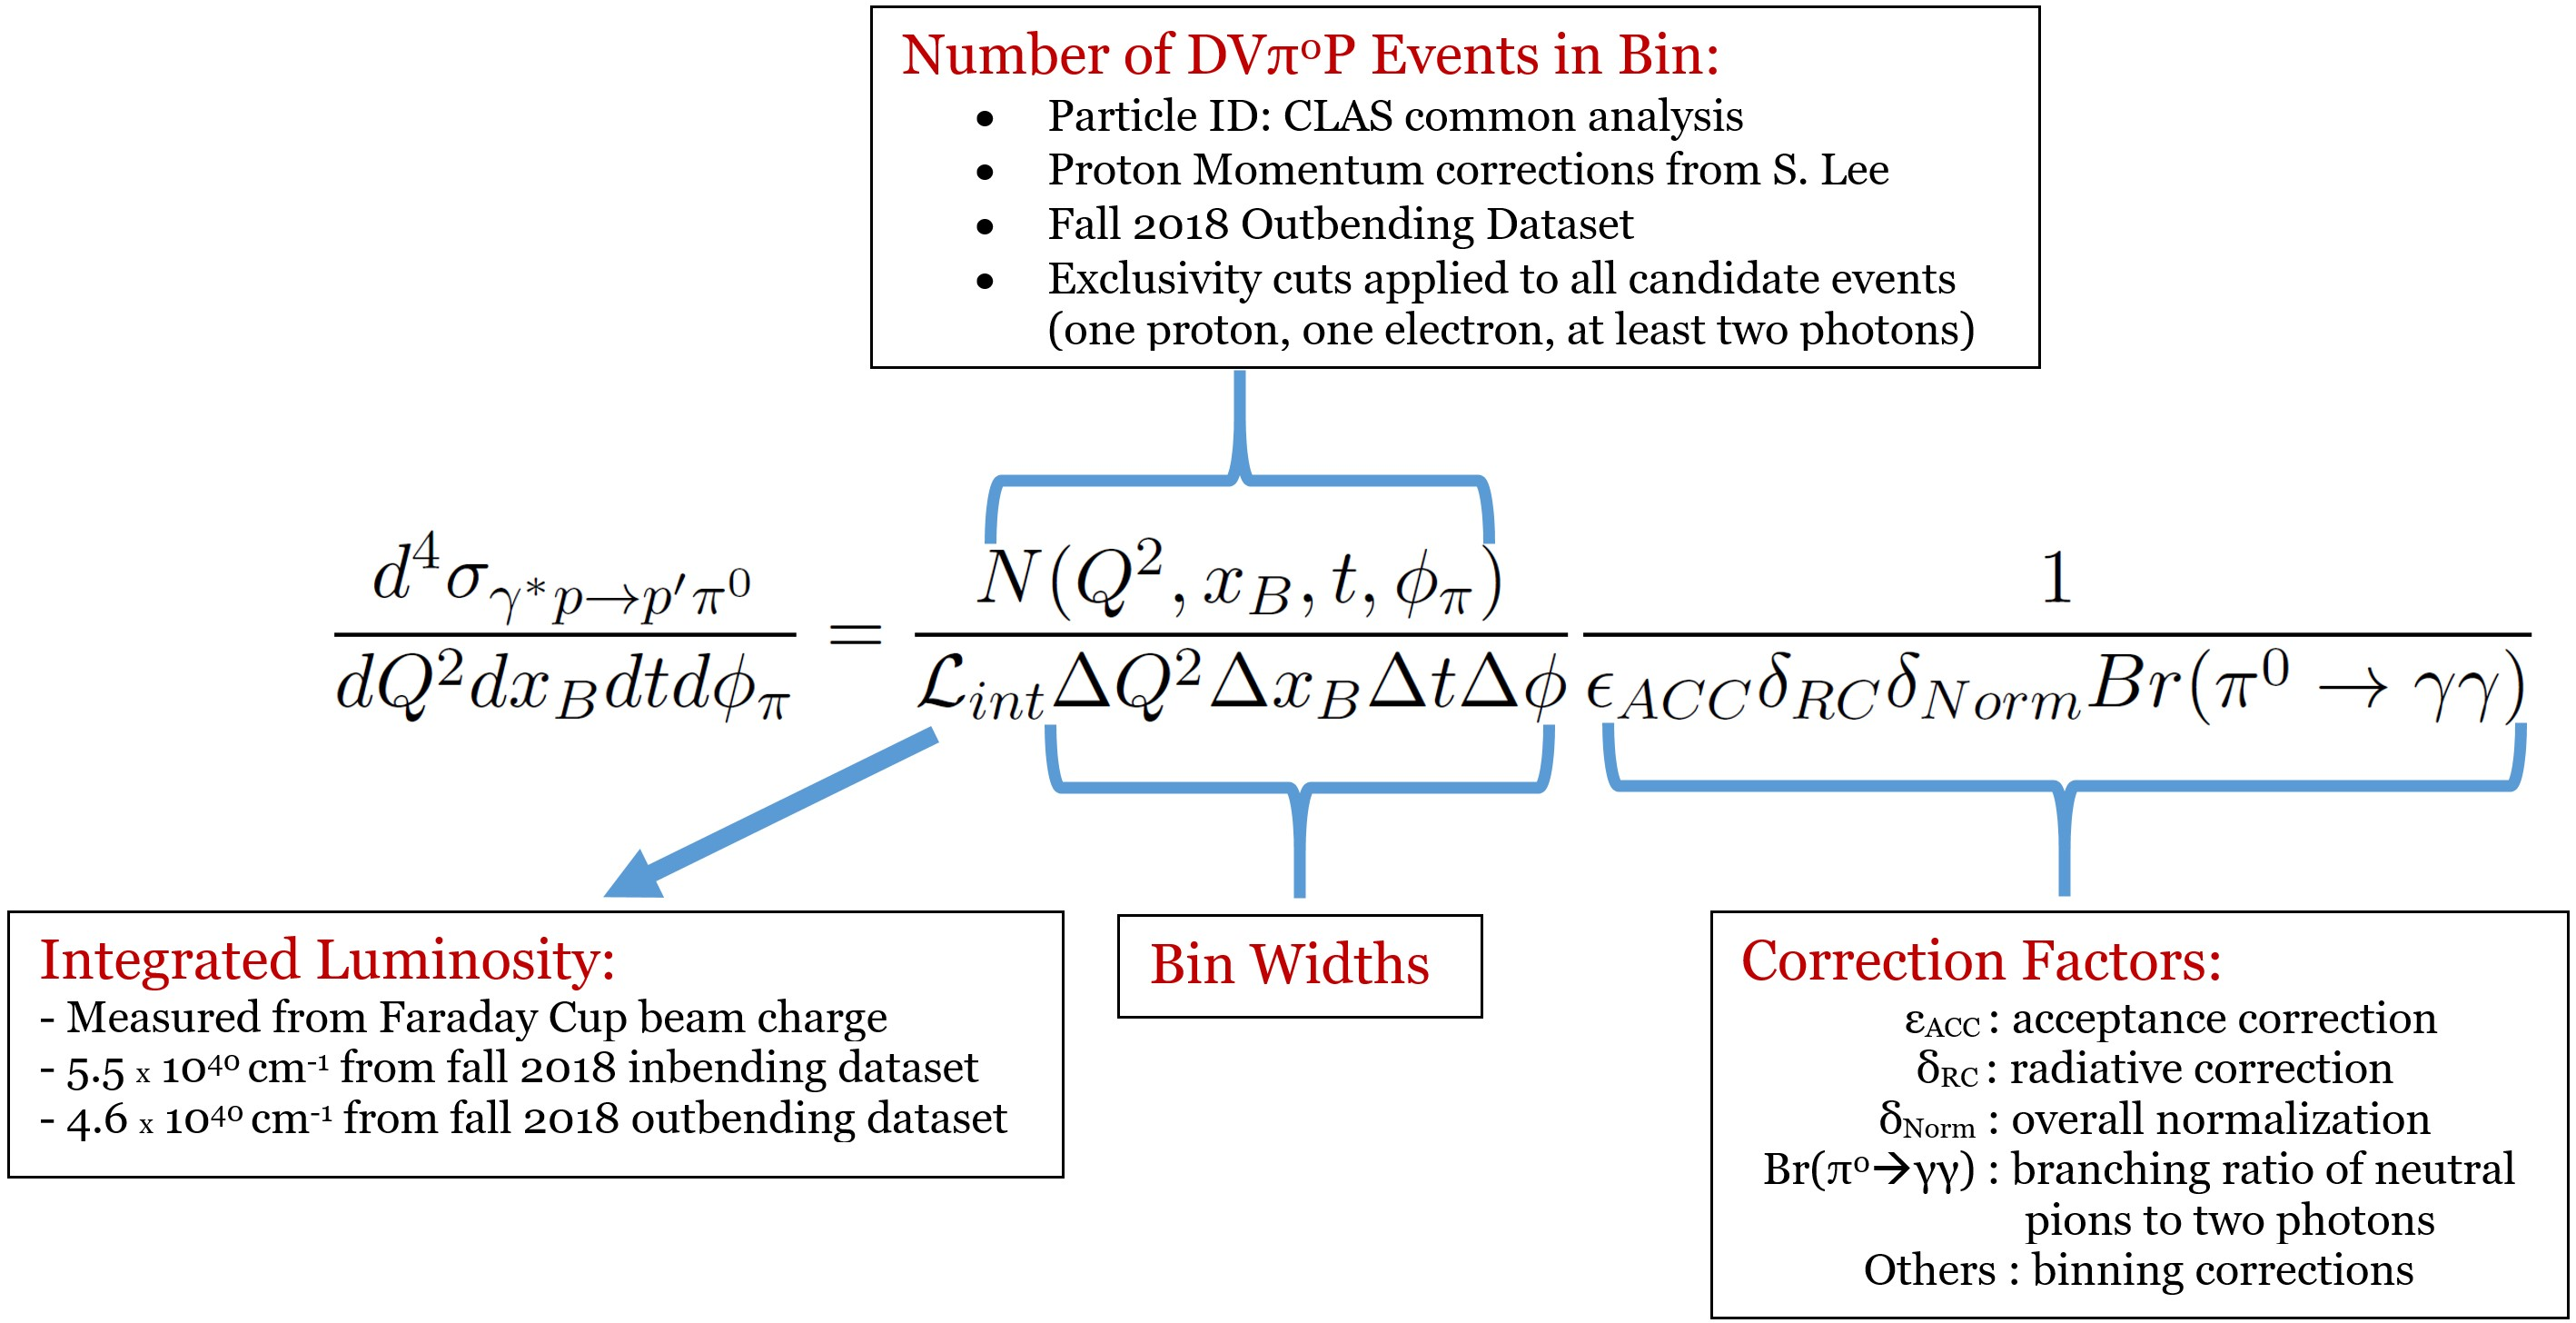
\includegraphics[trim={0 0  0 0cm} ,clip,width=.91725995\textwidth]{extra/steps3.jpg}

\end{frame}


\begin{frame}{Event Selection - Particle Identification and Exclusivity Cuts}

        
        \begin{columns}[c]
           \begin{column}{0.35\textwidth}
            \centering \textbf{\underline{Particle Kinematics}}
                %\vspace{1cm}
                \begin{itemize}
                    \item Electron
                        \begin{itemize}
                            \item Cherenkov Counter (PID)
                            \item Drift Chamber (momentum)
                            \item Time-of-flight (PID)
                            \item EM Calorimeter (energy)
                        \end{itemize}
                    \item Proton
                        \begin{itemize}
                            \item Time-of-flights (PID)
                            \item Micromegas, SVT, DCs (momentum)
                        \end{itemize}
                    \item Neutral Pion
                        \begin{itemize}
                            \item EM Calorimeter ($\gamma_1, \gamma_2$)
                            \item $ |M_{\pi^0} - M_{\gamma\gamma}| <$ 40 MeV
                        \end{itemize}
                \end{itemize}
                \end{column}
           %\hspace{-50pt}
            \vrule{}
            \begin{column}{0.65\textwidth}
            
            \centering  \textbf{\underline{Event Cuts}}
                    \begin{columns}[t, onlytextwidth]
            \column{0.45\textwidth}
                
                \begin{itemize}
                 \setlength\itemsep{0.5em}
                \item DIS Cuts
                   
                     \begin{itemize}
                     \setlength\itemsep{0.5em}
        
                    	\item  $Q^2 >$ 1 GeV$^2$
                    	\item W$^2 >$ 4 GeV$^2$
                		\end{itemize}
                		
                	\item Exclusivity Cuts
                	 \begin{itemize}
                     \setlength\itemsep{0.5em}	
                	\item $MM^2_{epX}<0.7$ GeV$^2$
                	
                	\item $M E_{ep \gamma \gamma}<0.7$ GeV

                	
                	\item $\theta_{X\pi}<2^\circ$
                	                	
                	\item $\Delta p_{x,y} <0.3$ GeV
                	\end{itemize}
                	\end{itemize}

        \column{0.55\textwidth}
                    %\textcolor{white}{blank space}

                
                        %#---------------------------------------------
                       	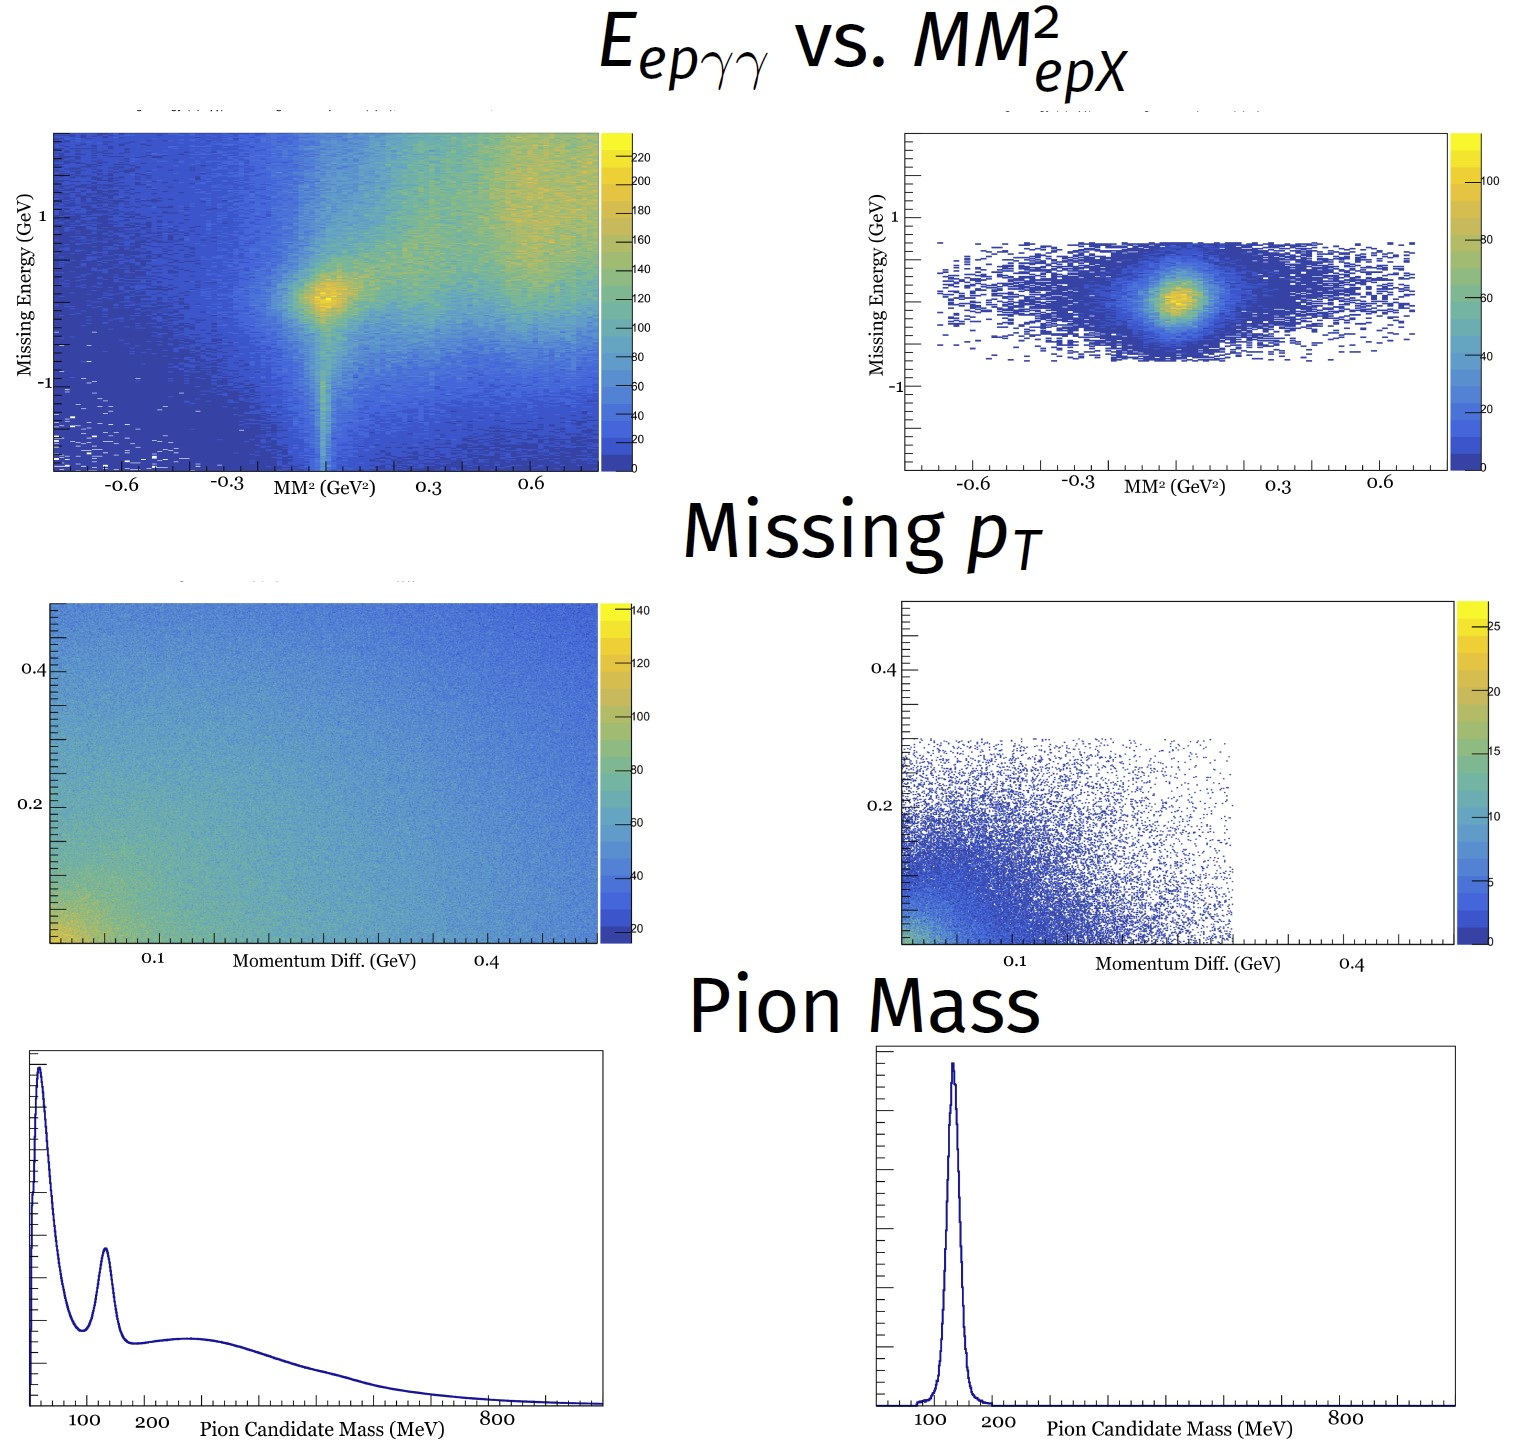
\includegraphics[trim={0 0  0 0cm} ,clip,width=.92\textwidth]{extra/exclusivity.jpg}

                	


        \end{columns}
        \end{column}   
        \end{columns}
\end{frame}

\begin{frame}
    cuts are restrictive
    TALK ABOUT EIC
\end{frame}

\begin{frame}{Computational Resources}
    Jefferson Lab Pic
\end{frame}

\begin{frame}{Computational Resources}
    Bates OSG Pipeline
\end{frame}

\begin{frame}{Acceptance Correction - Event Generator and Simulation}
     \begin{columns}[c]
               \begin{column}{0.5\textwidth}

                    %\vspace{1cm}
                    \begin{itemize}
                        \item Event Generator - aao\_norad
                            \begin{itemize}
                                \item Nonradiative $DV\pi^0P$ generator validated on CLAS6 and COMPASS data
                            \end{itemize}
                        \item Simulation - GEMC
                            \begin{itemize}
                                \item GEANT4 based simulation developed by CLAS collaboration
                            \end{itemize}
                        \item Computing Power
                            \begin{itemize}
                                \item Through OSG pipeline, CLAS has access to supercomputing clusters around the world, including dedicated nodes at MIT Tier 2, UConn, INFN, GRIDPP, and more
                            \end{itemize}
                    \end{itemize}
                    \end{column}
                    
                    
    \begin{column}{0.5\textwidth}
                
                \centering Generated \\
        \begin{columns}
                    
                    \column{0.5\textwidth}
                        %\textcolor{white}{blank space}
                             
                    
                            %#---------------------------------------------
                           	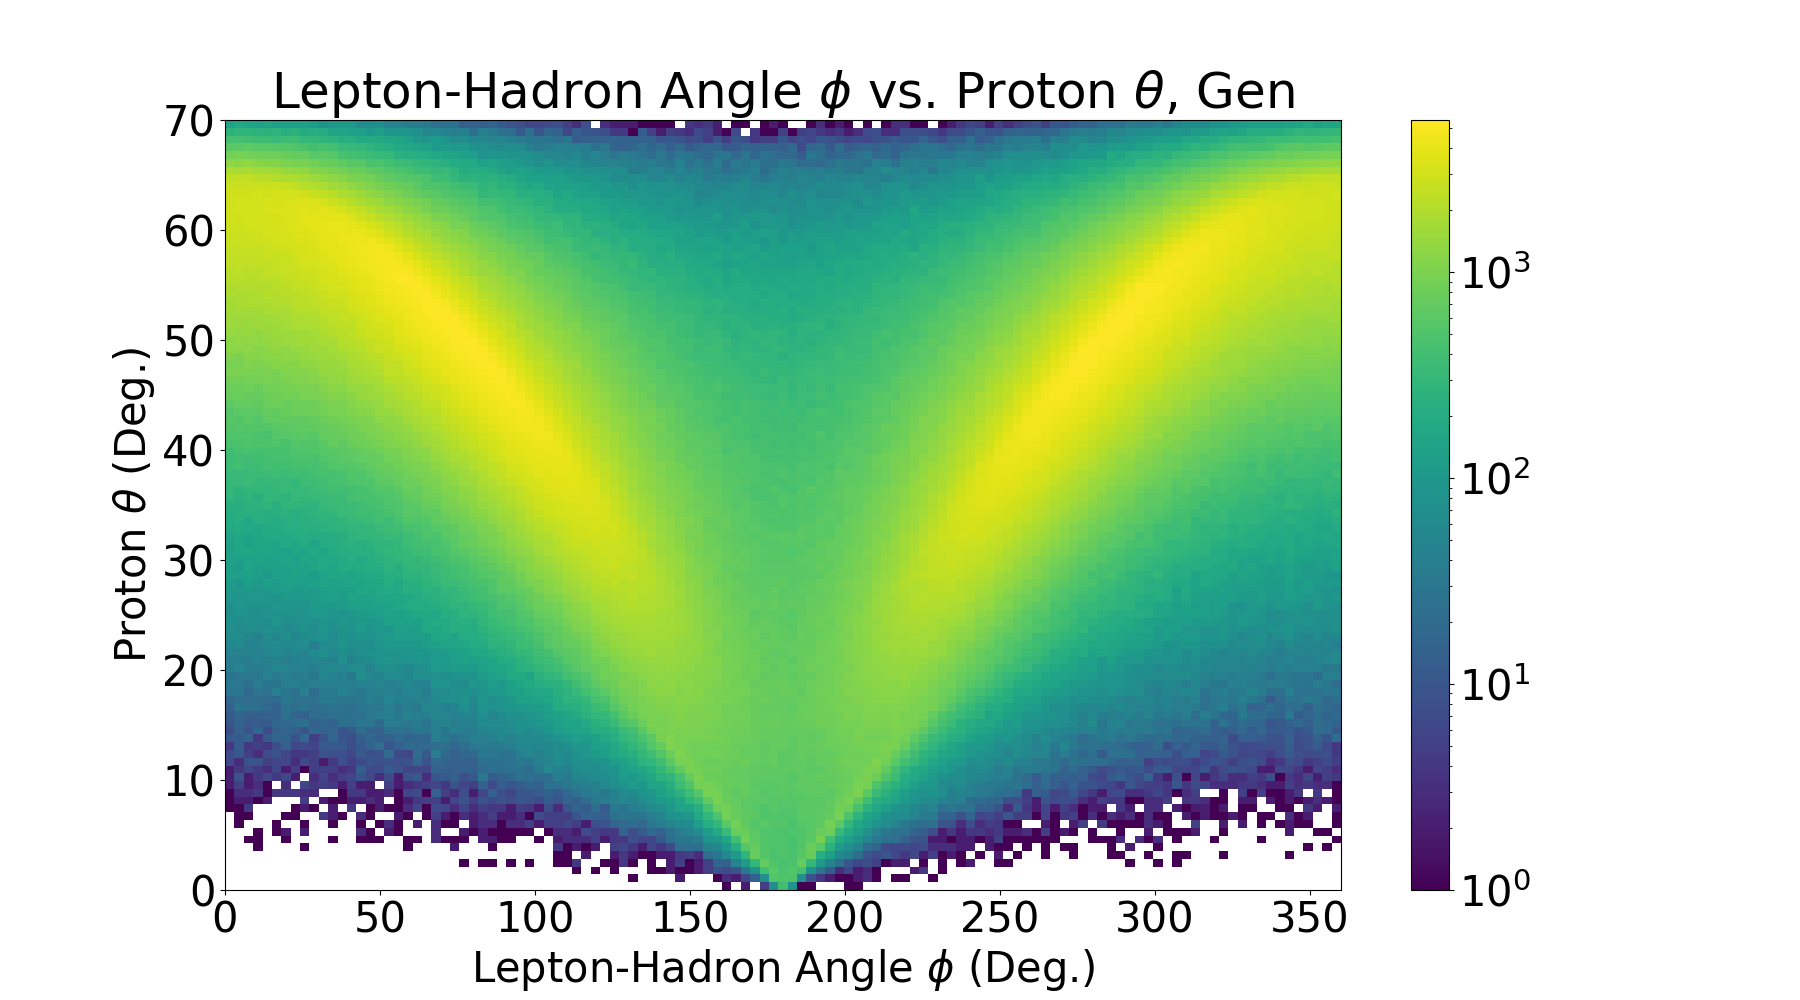
\includegraphics[trim={0 0  0 0cm} ,clip,width=.982\textwidth]{extra/generator/Lepton-Hadron_Angle_phi_vs_Proton_theta,_Gen.png}
                           	   
                  \column{0.5\textwidth}          	   
                           	
                        	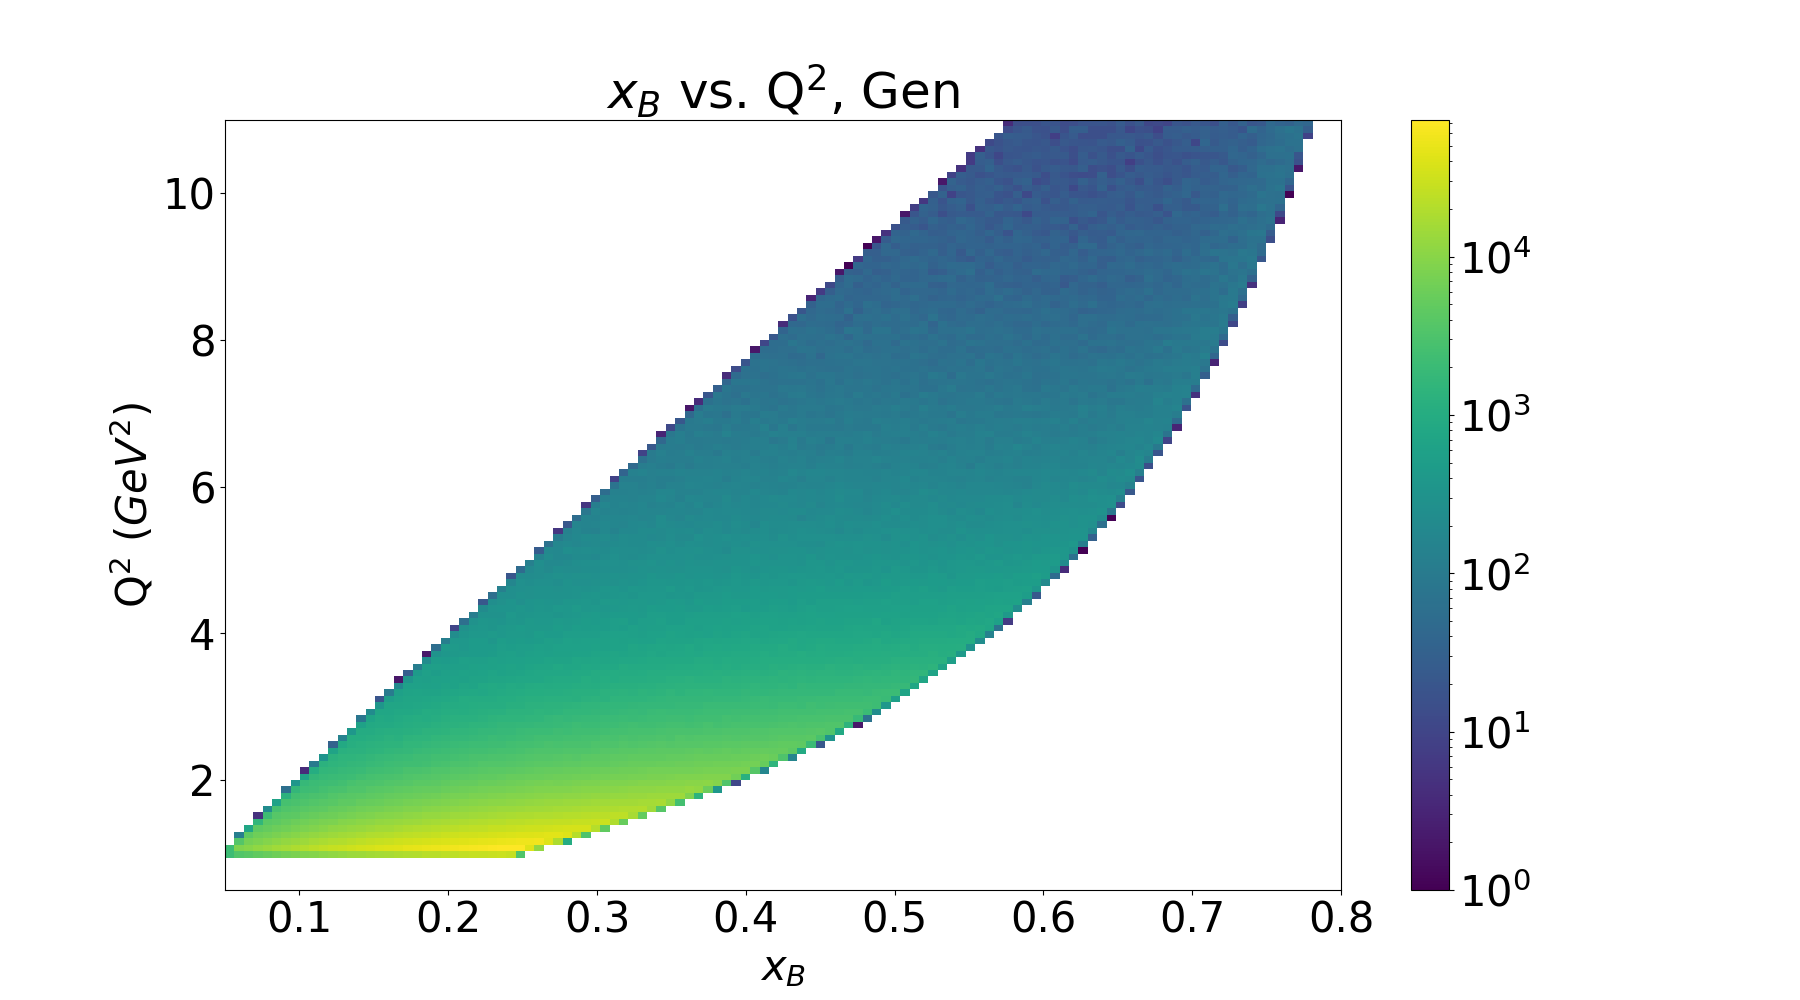
\includegraphics[trim={0 0  0 0cm} ,clip,width=.982\textwidth]{extra/generator/x_B_vs_Q2,_Gen.png}
            
                        \end{columns}
                        \vspace{0.3cm}
              \centering Reconstructed \\      
          \begin{columns} 
            
            
                        \column{0.5\textwidth}
             
                               
                           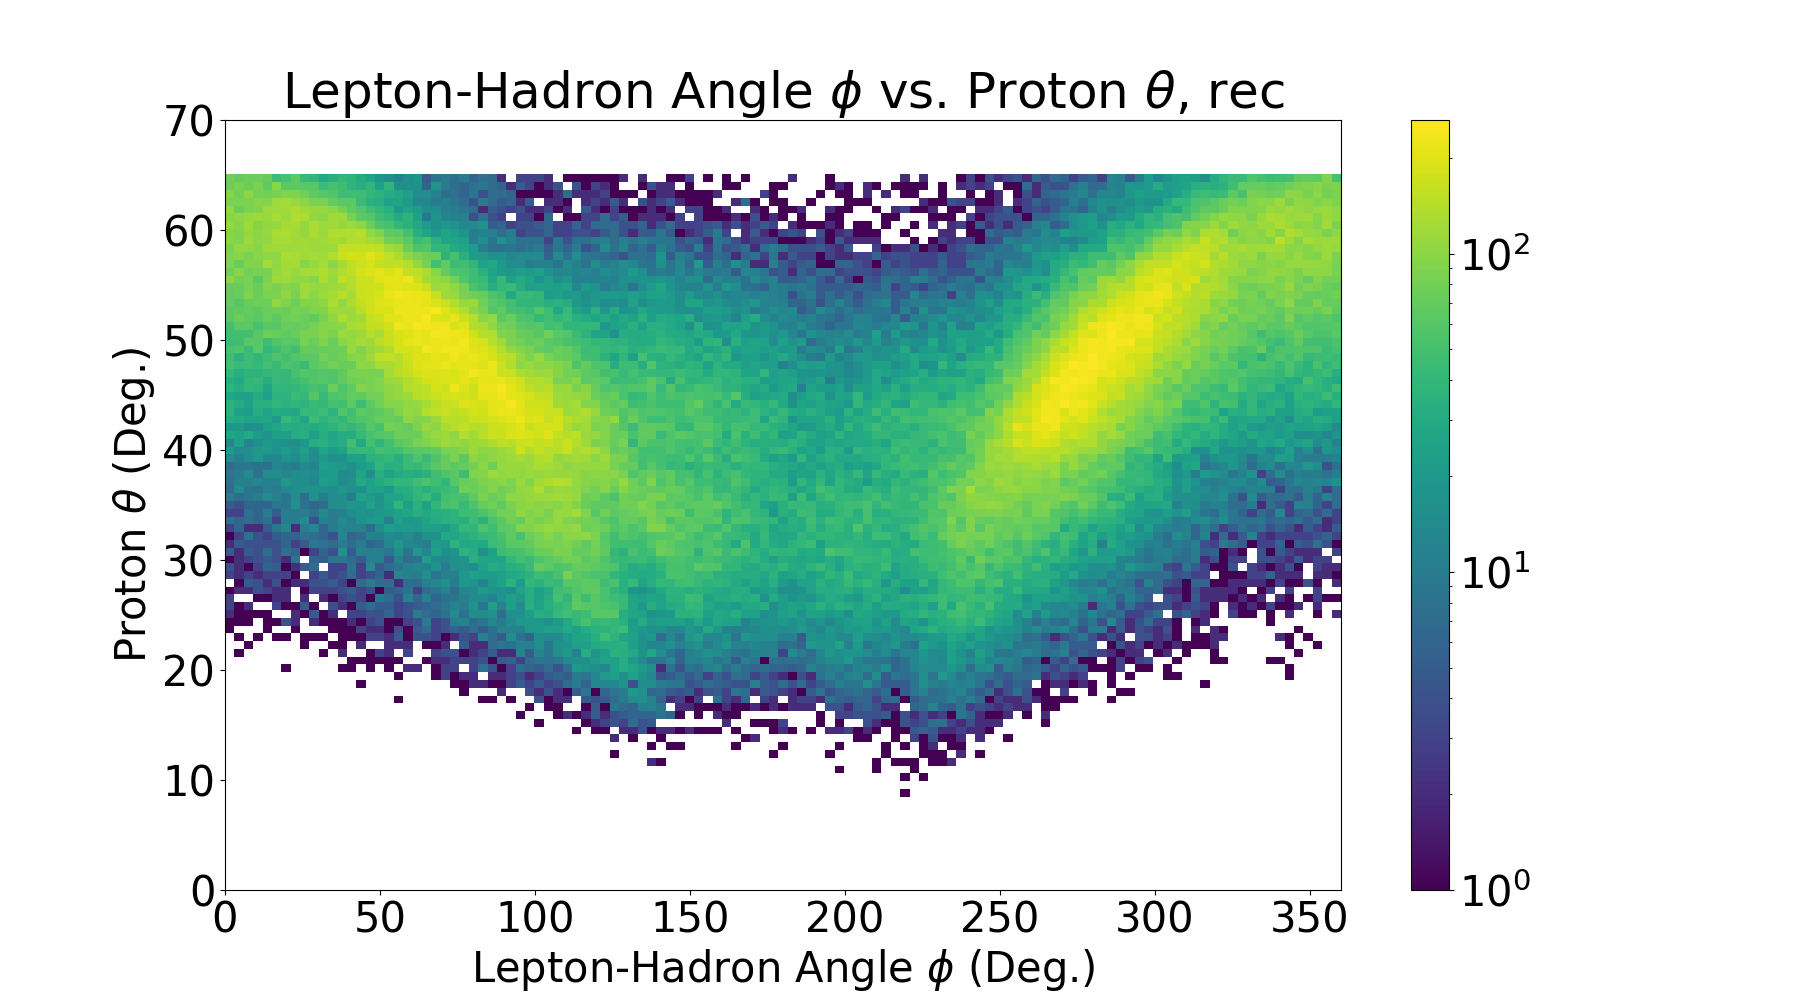
\includegraphics[trim={0 0  0 0cm} ,clip,width=.982\textwidth]{extra/generator/Lepton-Hadron_Angle_phi_vs_Proton_theta,_rec.png}
           \column{0.5\textwidth}
                              
                        	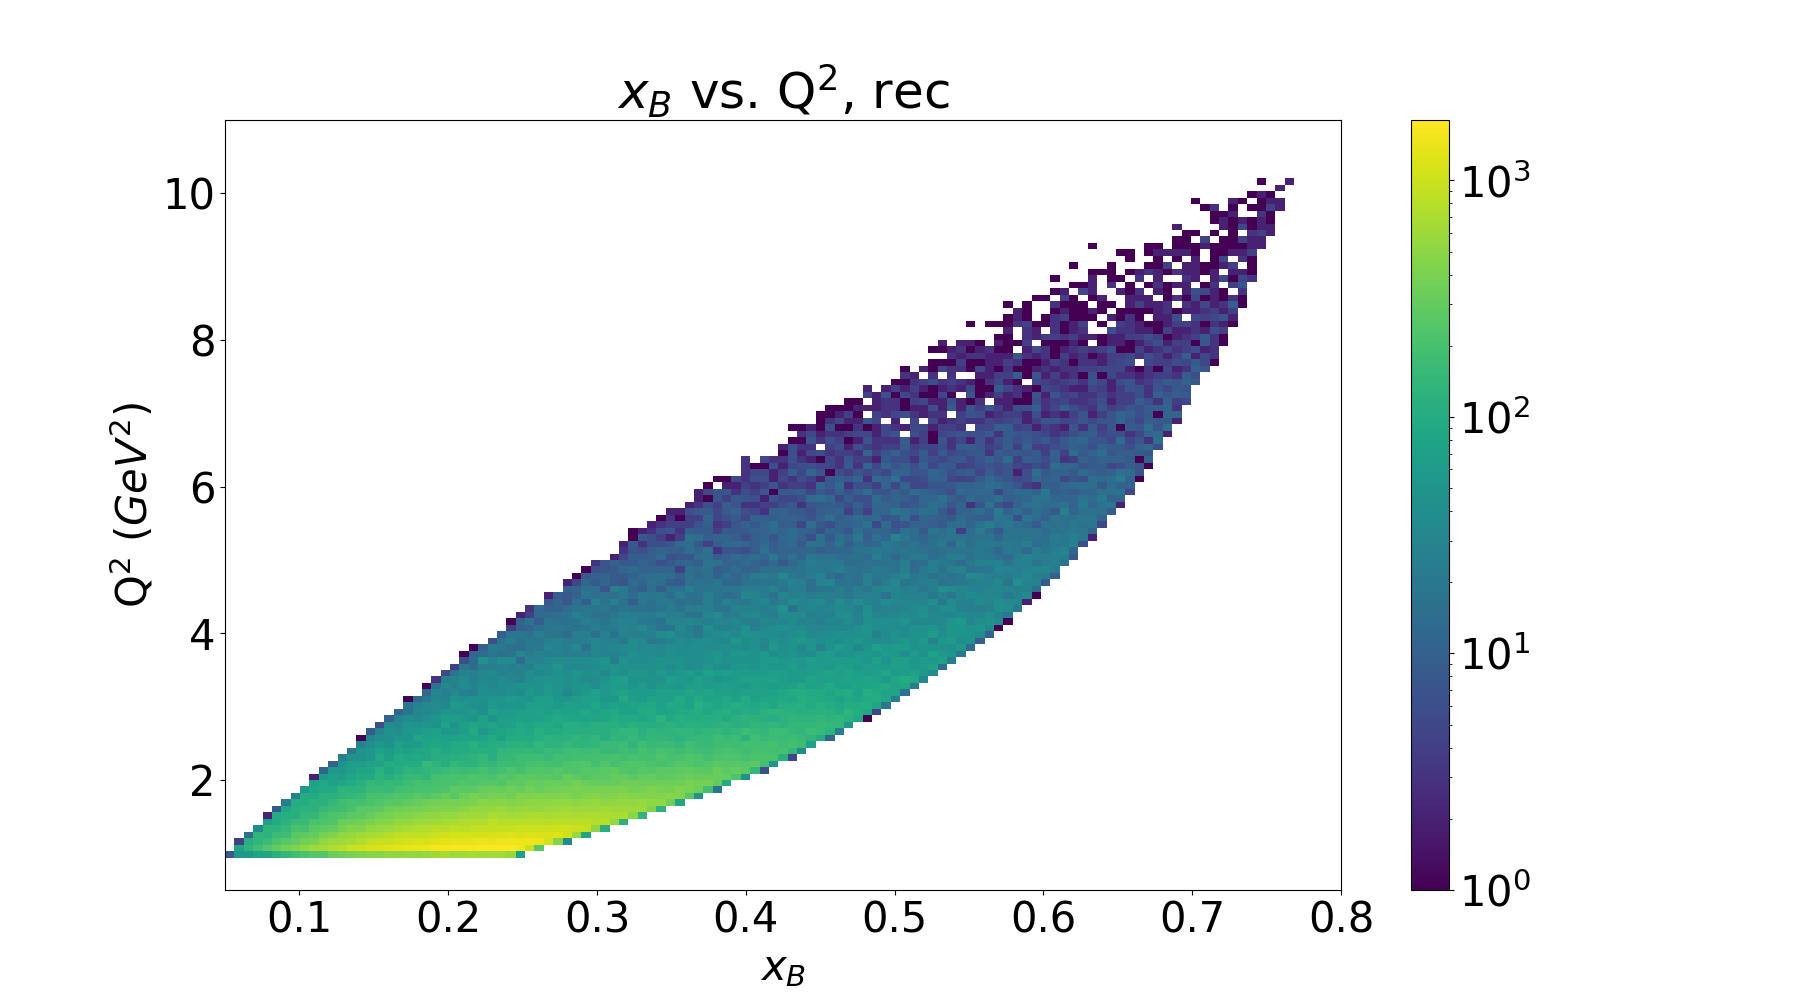
\includegraphics[trim={0 0  0 0cm} ,clip,width=.982\textwidth]{extra/generator/x_B_vs_Q2,_rec.png}
        
                \end{columns}
    \end{column}
                    
    \end{columns}
\end{frame}

\begin{frame}{Acceptance Correction - Simulation : Experiment Matching}

With the addition of smearing factors to simulated particle reconstruction values, the simulation matches experimental distributions well.  {\myfont{\footnotesize [Collaborator S. Lee]}}




\vspace{0.2cm}
\begin{columns}
            \column{0.32\textwidth}
                %\textcolor{white}{blank space}
                     \centering $ME_{ep\gamma\gamma}$ \\
                        % trim={<left> <lower> <right> <upper>}
                    %#---------------------------------------------
                   	\includegraphics[trim={0 1.75cm  0 3.05cm} ,clip,width=.82\textwidth]{simcomp/yessmear/outbending_rad_All_All_All_for_aps_2022_plots_sangcutsME_epgg_exp_vs_sim.png}
                   	   \centering  $MM^2_{e\gamma\gamma}$ \\
                	\includegraphics[trim={0 1.75cm  0 3.05cm} ,clip,width=.82\textwidth]{simcomp/yessmear/outbending_rad_All_All_All_for_aps_2022_plots_sangcutsMM2_egg_exp_vs_sim.png}


                \column{0.32\textwidth}
     
                       \centering  $MM^2_{ep\gamma\gamma}$ \\
                	\includegraphics[trim={0 1.75cm  0 3.05cm} ,clip,width=.82\textwidth]{simcomp/yessmear/outbending_rad_All_All_All_for_aps_2022_plots_sangcutsMM2_epgg_exp_vs_sim.png}
   
                      \centering   $MM^2_{ep}$ \\
                	\includegraphics[trim={0 1.75cm  0 3.05cm} ,clip,width=.82\textwidth]{simcomp/yessmear/outbending_rad_All_All_All_for_aps_2022_plots_sangcutsMM2_ep_exp_vs_sim.png}

            
            \column{0.32\textwidth}

                    %#---------------------------------------------
                      \centering   $M_{\gamma\gamma}$ \\
                	\includegraphics[trim={0 1.75cm  0 3.05cm} ,clip,width=.82\textwidth]{simcomp/yessmear/outbending_rad_All_All_All_for_aps_2022_plots_sangcutsMpi0_exp_vs_sim.png}
 
                       \centering  $\Delta p_{t}$ \\
                	\includegraphics[trim={0 1.75cm  0 3.05cm} ,clip,width=.82\textwidth]{simcomp/yessmear/outbending_rad_All_All_All_for_aps_2022_plots_sangcutsMPt_exp_vs_sim.png}

    \end{columns}
\end{frame} 


\begin{frame}{Acceptance Correction - Bin by Bin Calculation}
\begin{columns}
            \column{0.25\textwidth}
                %\textcolor{white}{blank space}
                     \centering Raw Counts \\
            
                    %#---------------------------------------------
                   	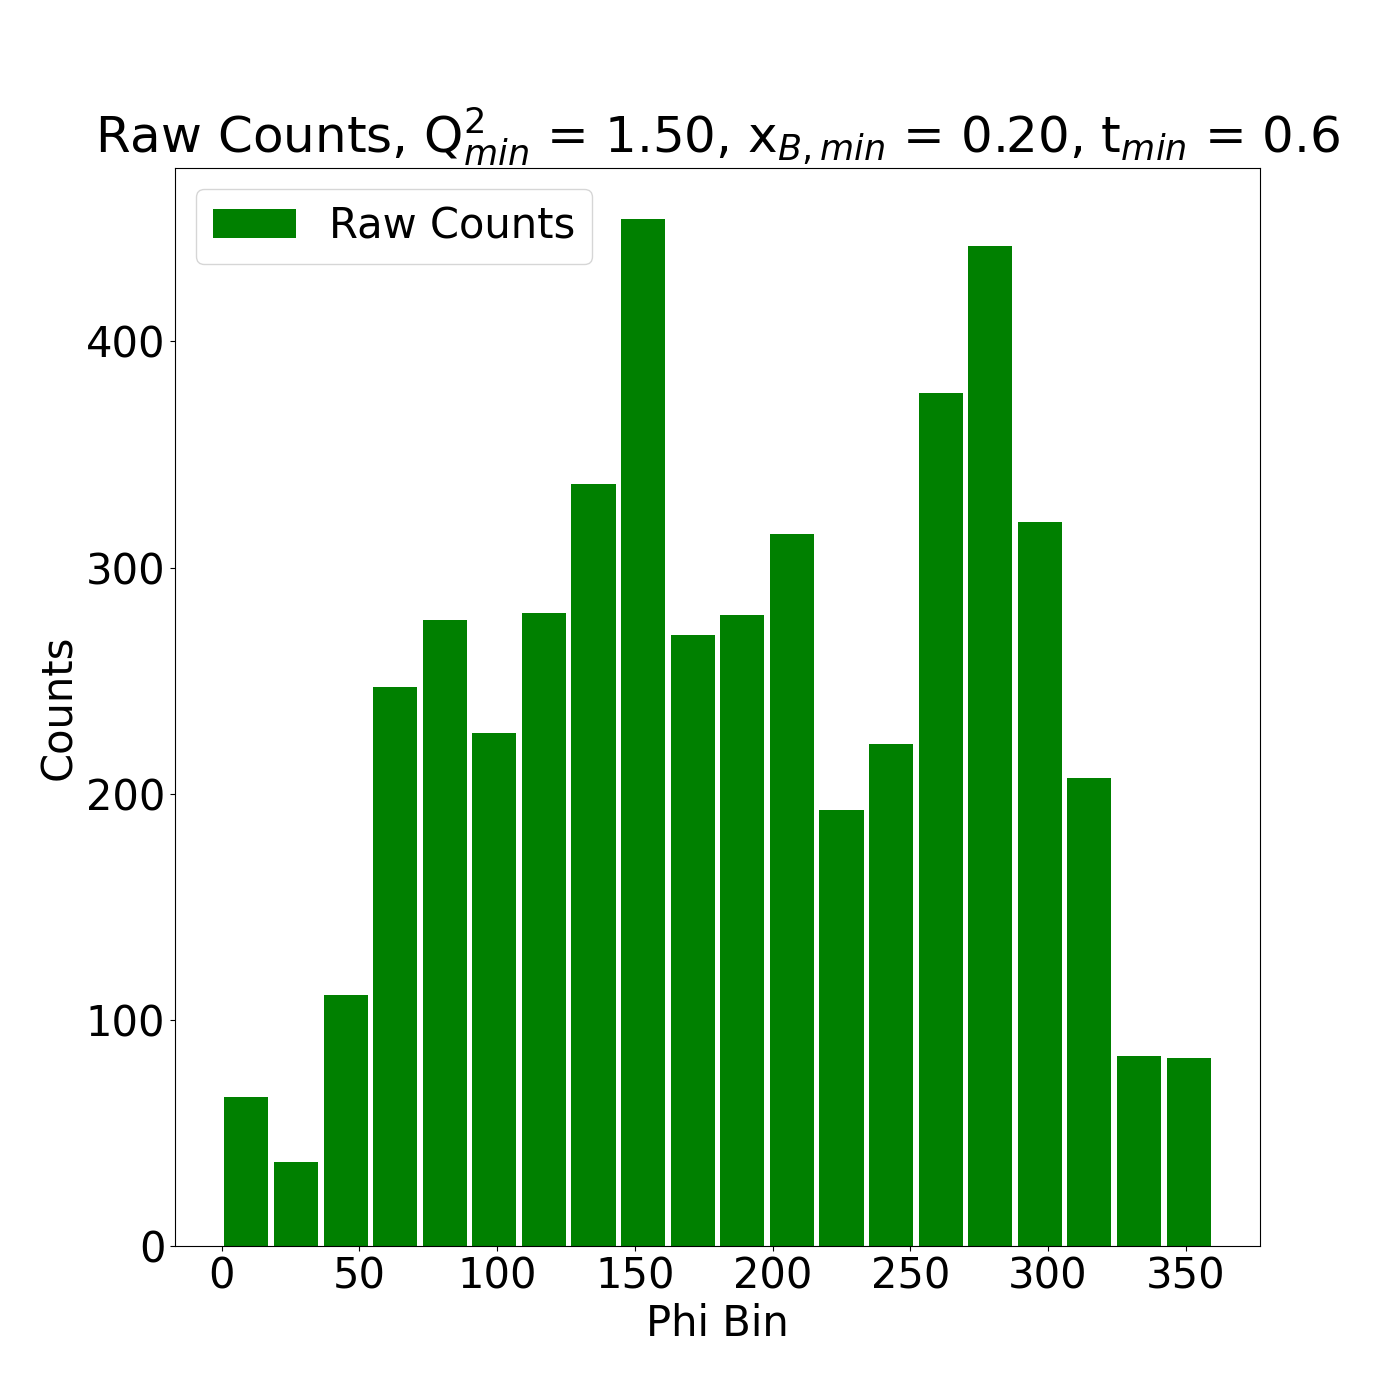
\includegraphics[trim={0 0  0 0cm} ,clip,width=.8982\textwidth]{extra/corrs/raw2.png}


                   	
                	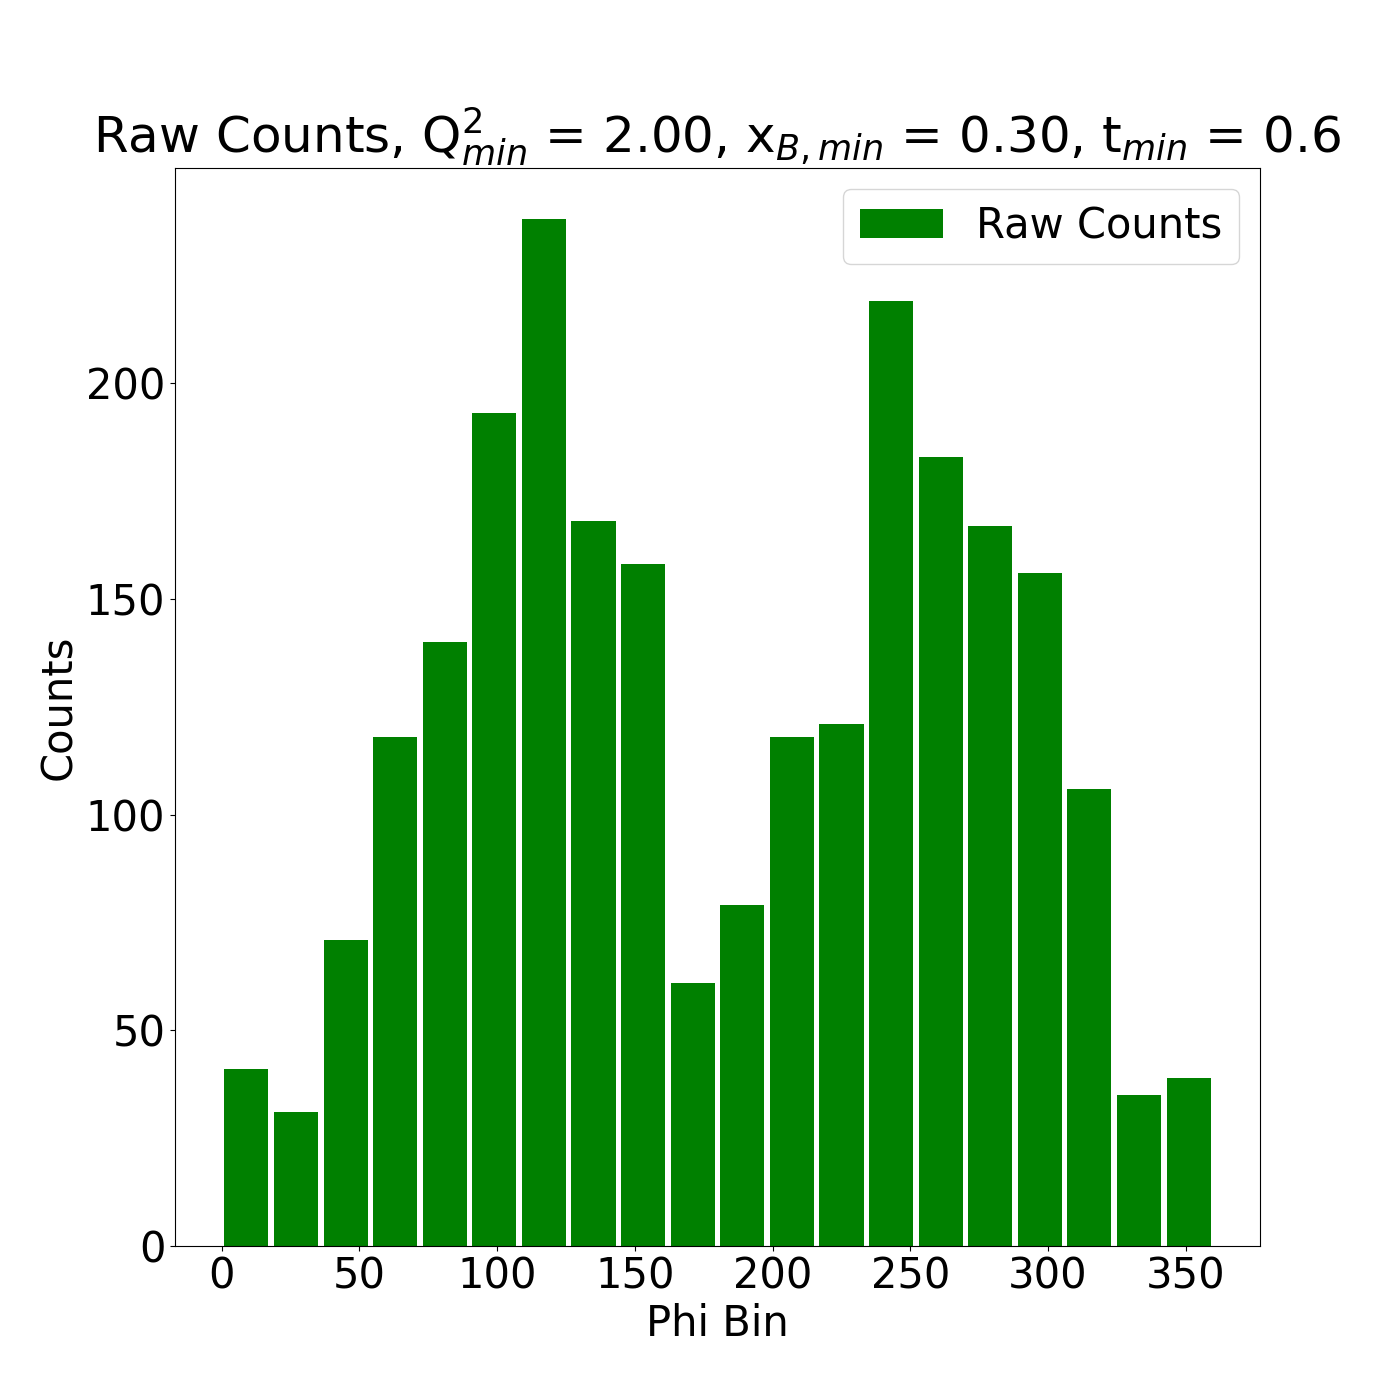
\includegraphics[trim={0 0  0 0cm} ,clip,width=.8982\textwidth]{extra/corrs/raw4.png}


                \column{0.25\textwidth}
     
                       \centering  Simulated $N_{Gen}$, $N_{Rec}$ \\
                	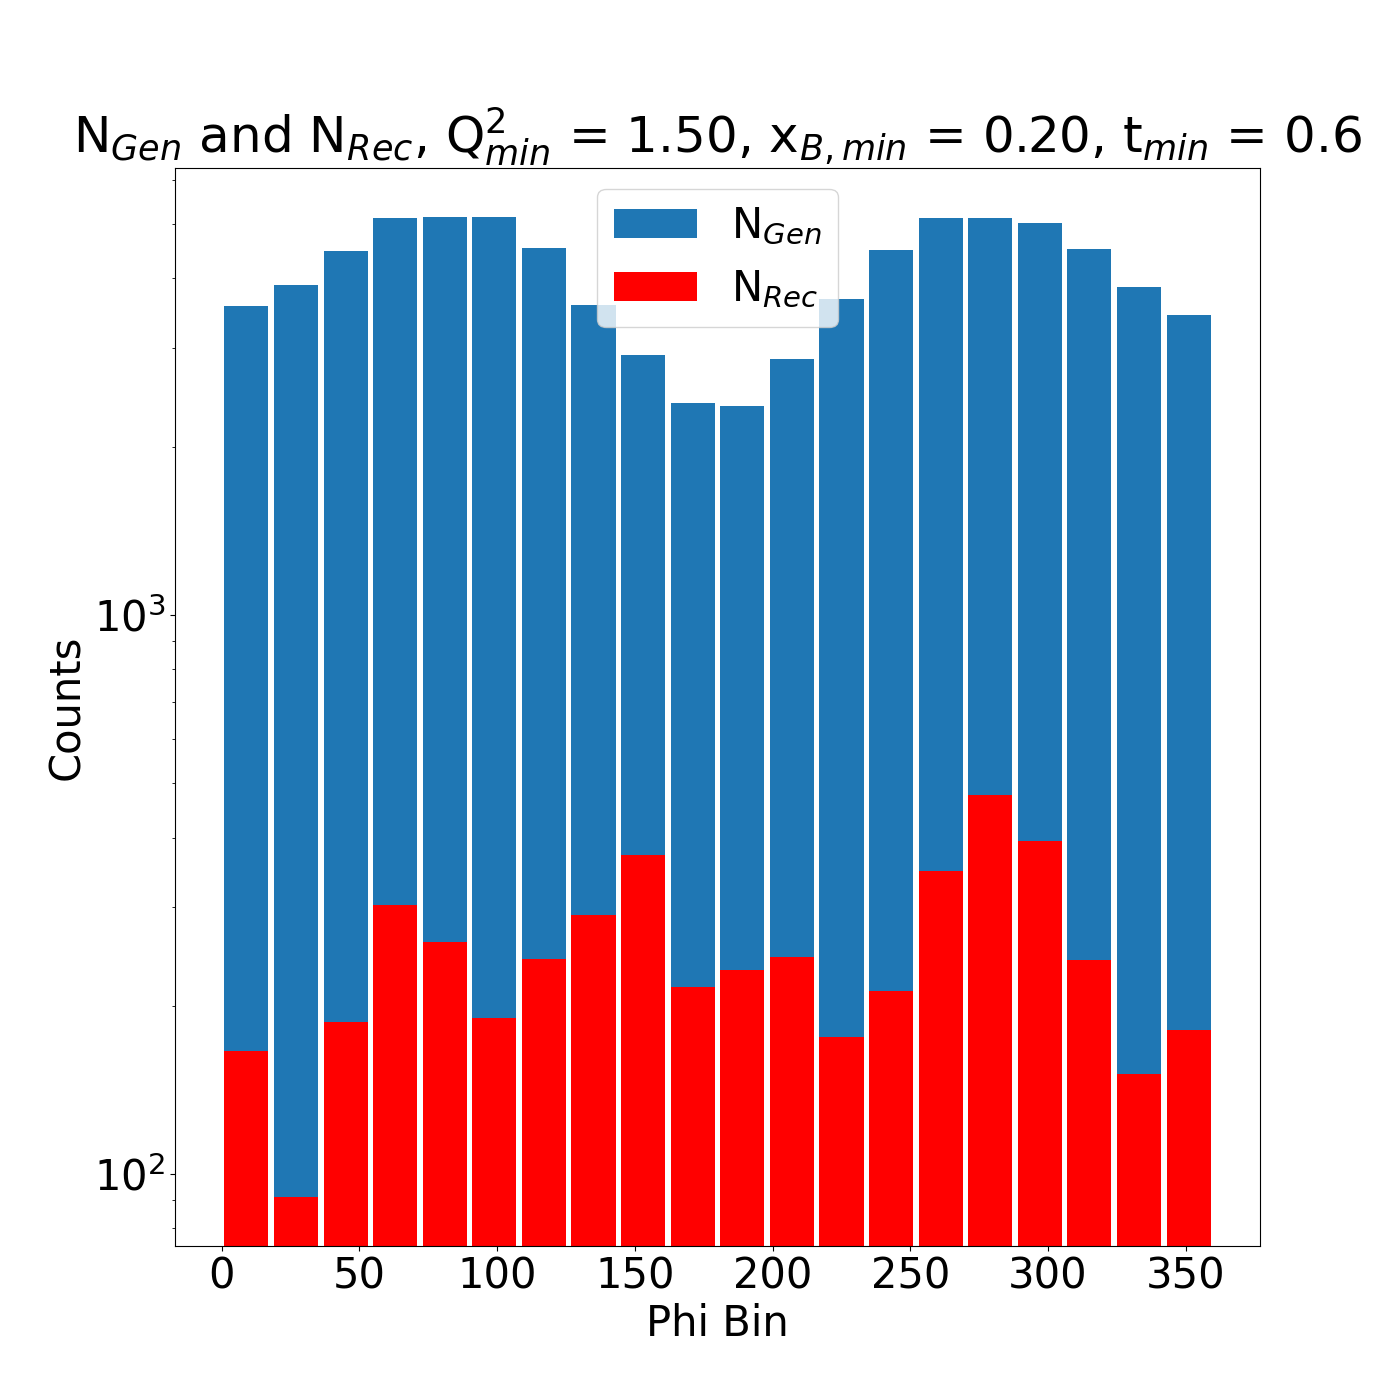
\includegraphics[trim={0 0  0 0cm} ,clip,width=.8982\textwidth]{extra/corrs/acc2.png}
   
                    
                	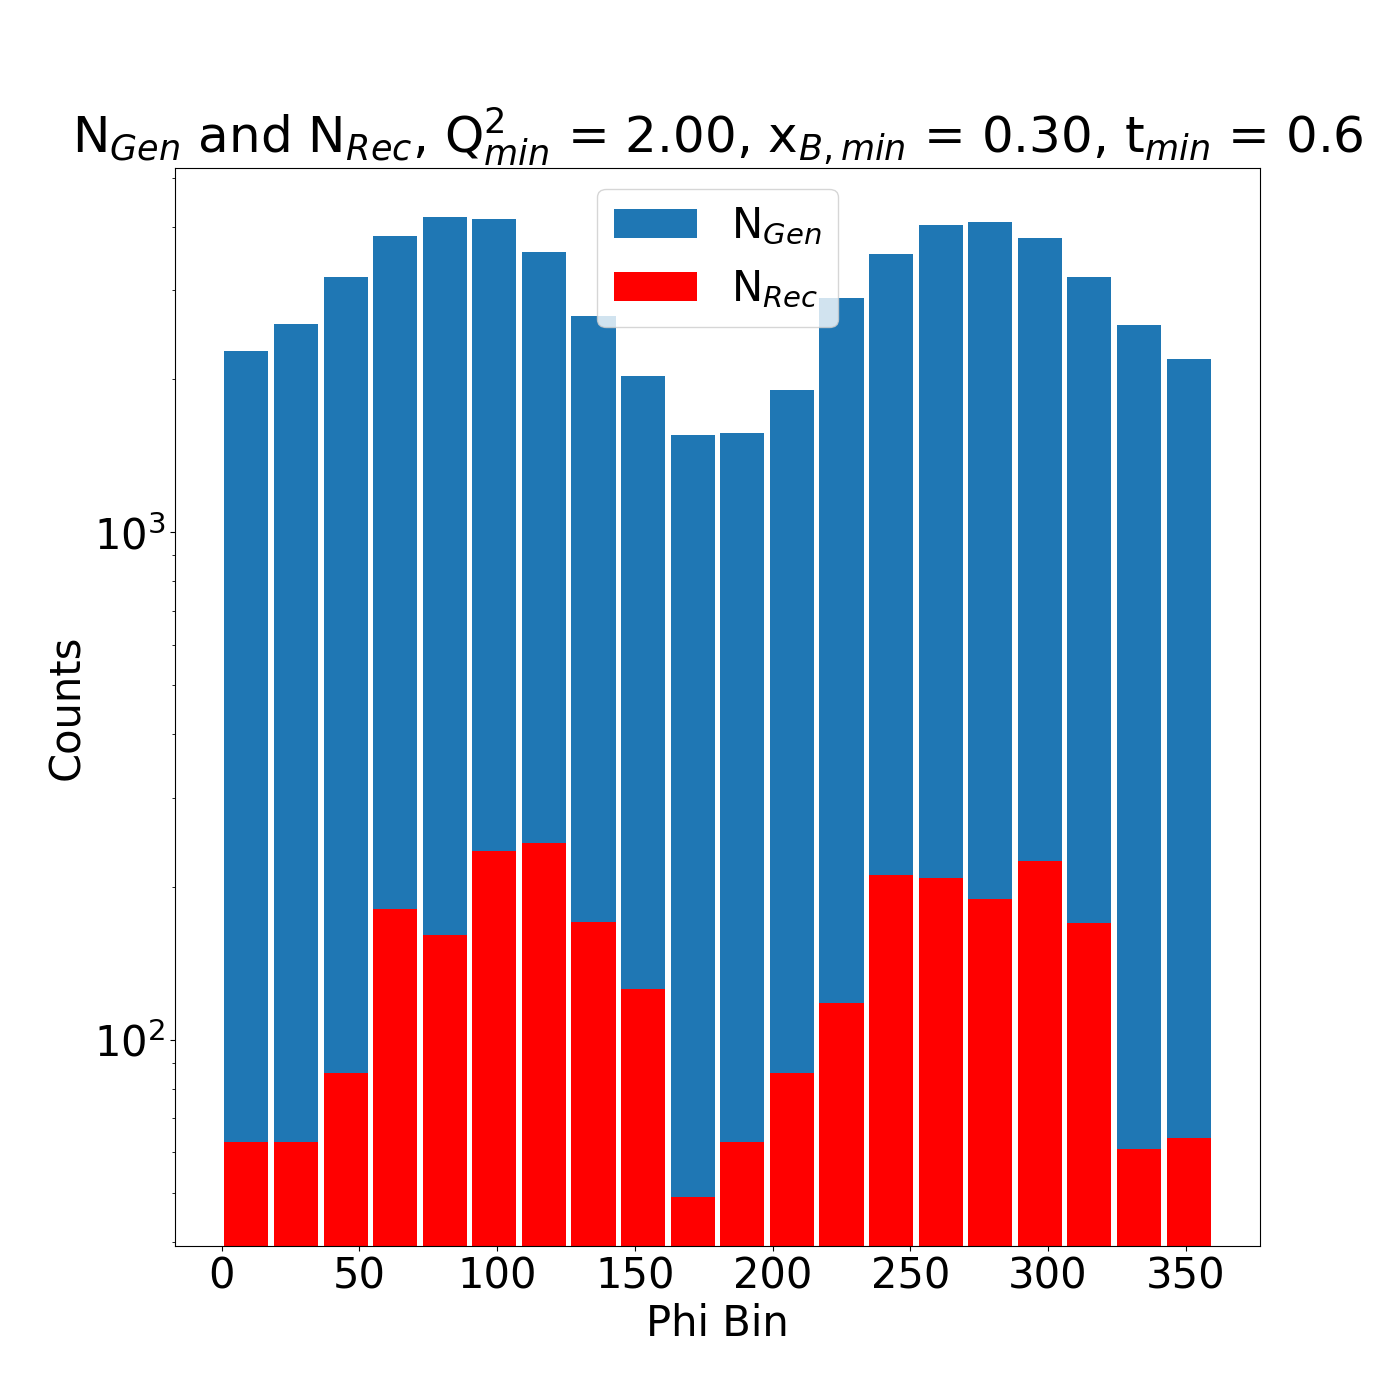
\includegraphics[trim={0 0  0 0cm} ,clip,width=.8982\textwidth]{extra/corrs/acc4.png}

            
            \column{0.25\textwidth}

                    %#---------------------------------------------
                      \centering   Acc. Correction \\
                	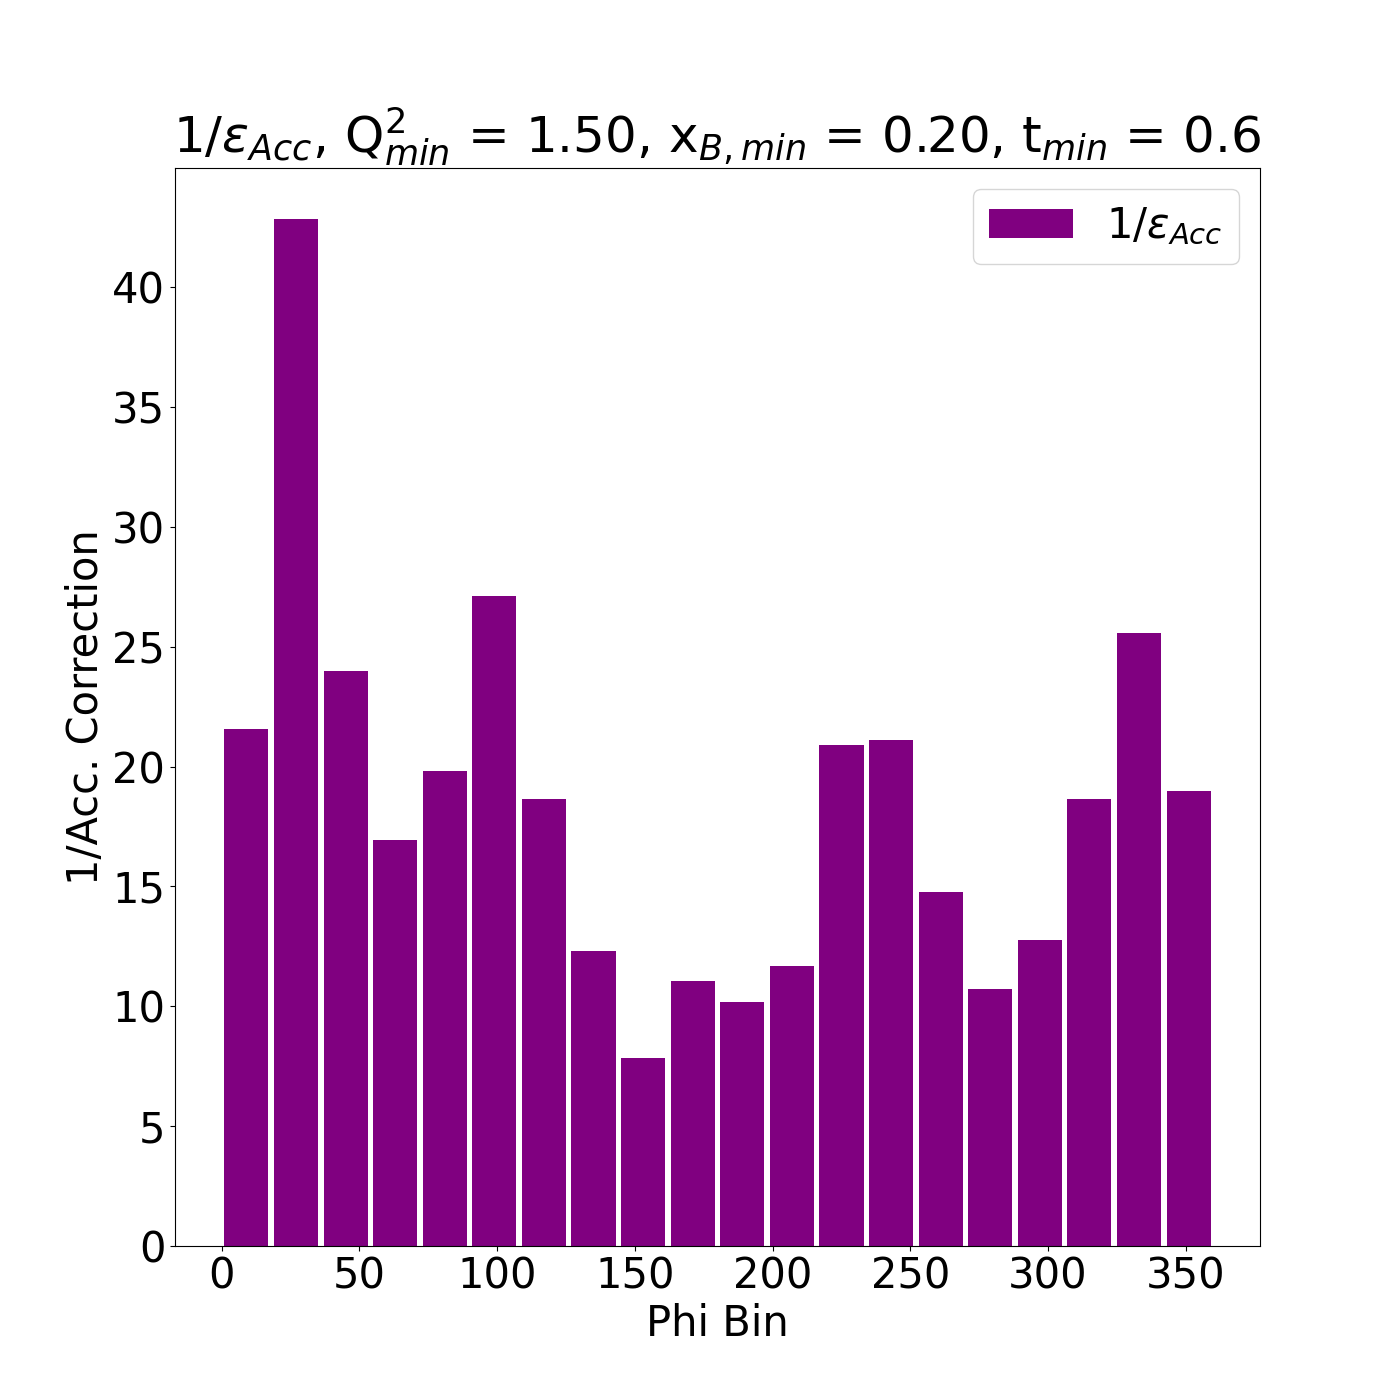
\includegraphics[trim={0 0  0 0cm} ,clip,width=.8982\textwidth]{extra/corrs/raw2acc.png}
 
             
                	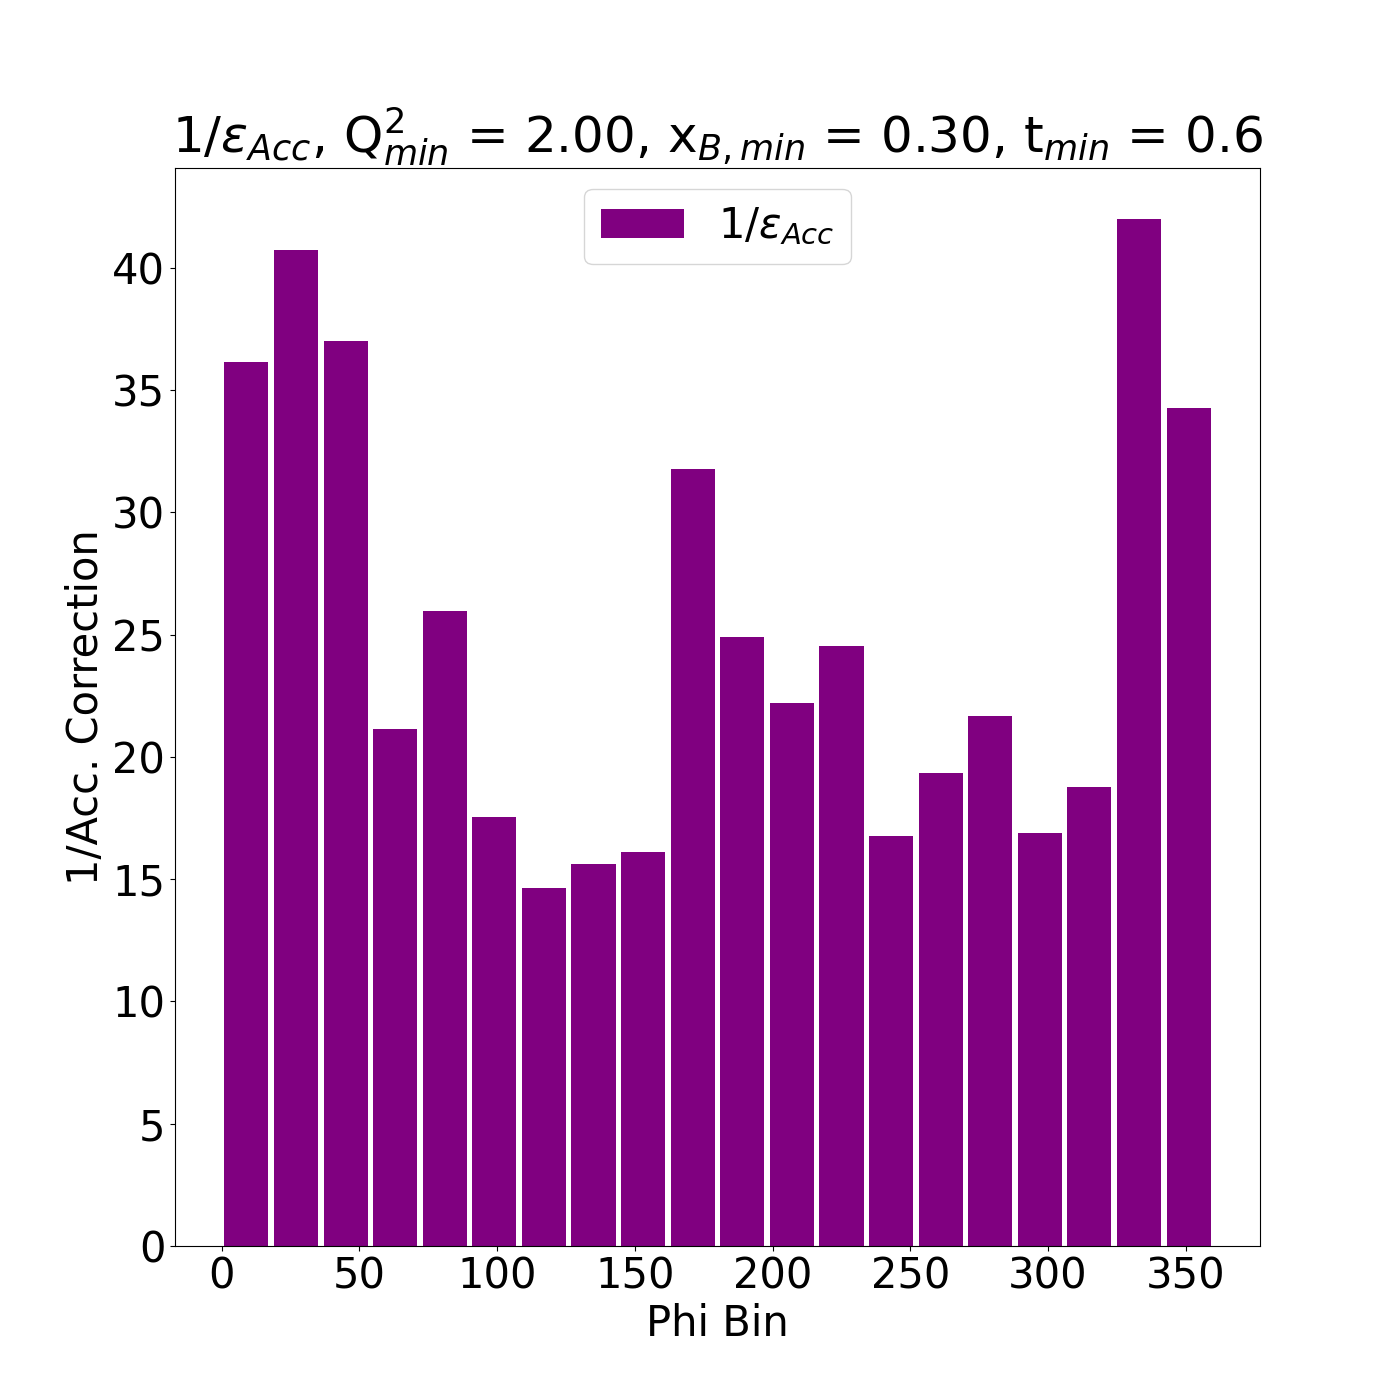
\includegraphics[trim={0 0  0 0cm} ,clip,width=.8982\textwidth]{extra/corrs/acc_3.png}
                	
                	
            \column{0.25\textwidth}

                    %#---------------------------------------------
                      \centering   Acc. Corr. Counts \\
                	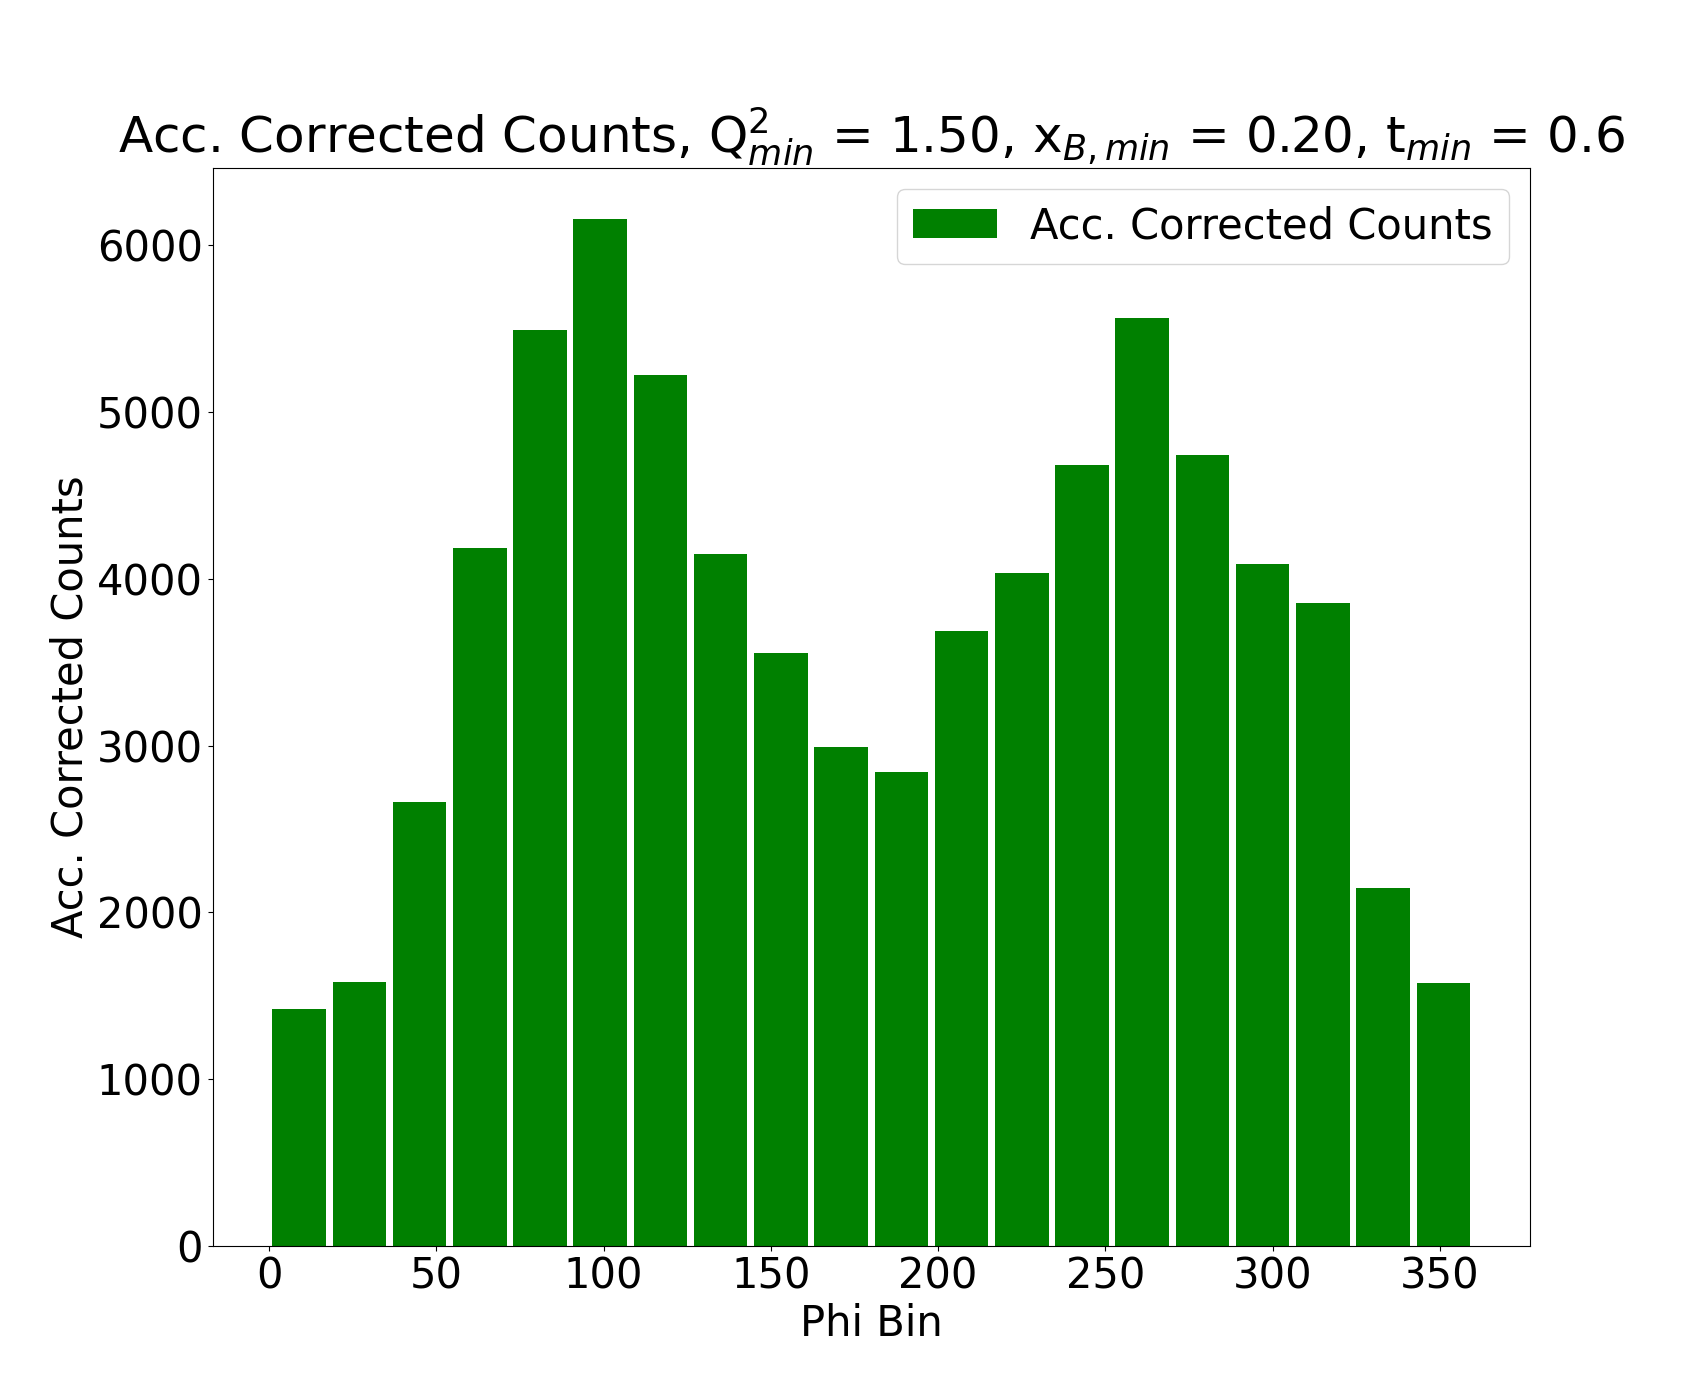
\includegraphics[trim={0 0  0 0cm} ,clip,width=.982\textwidth]{extra/corrs/final1.png}
 
       
                	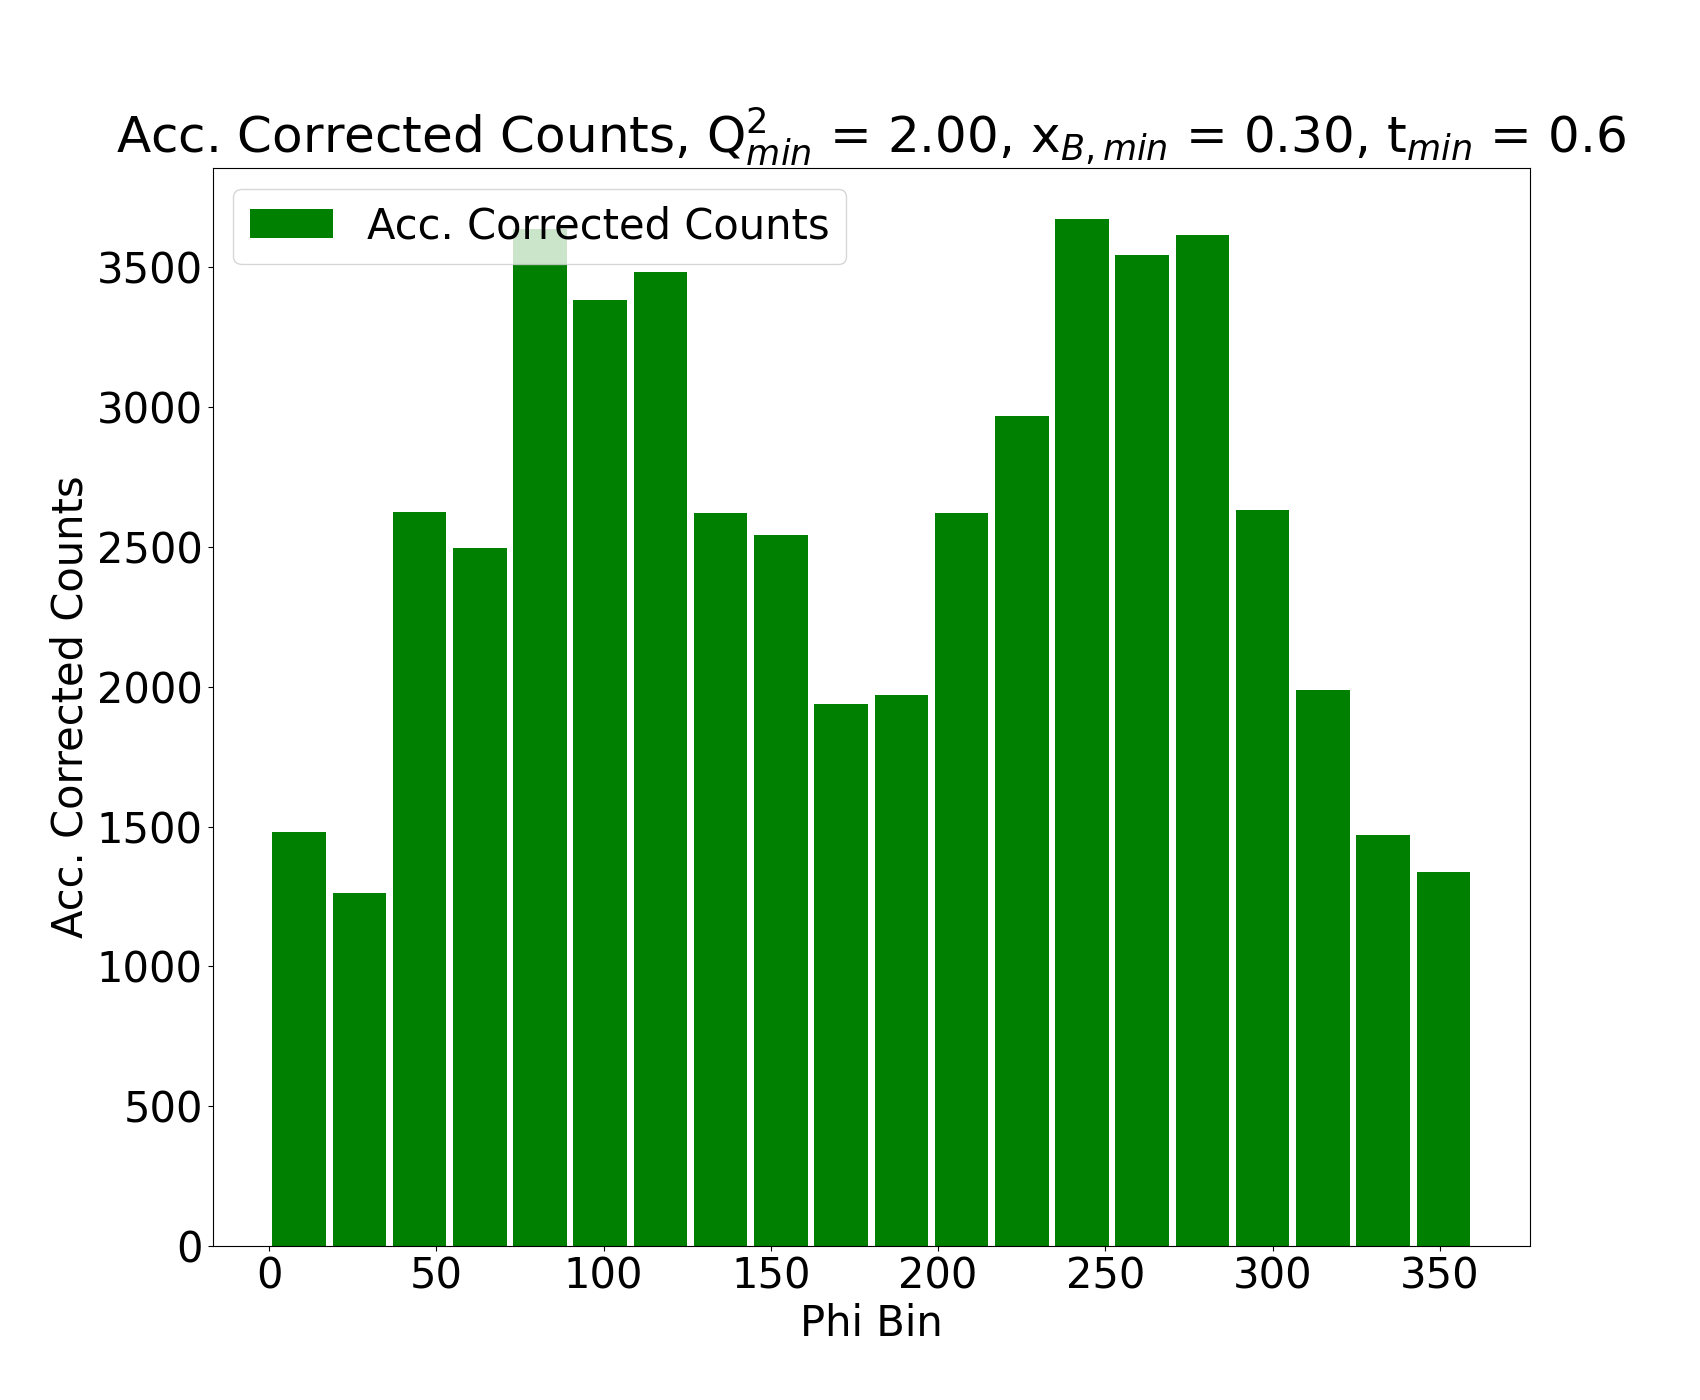
\includegraphics[trim={0 0  0 0cm} ,clip,width=.982\textwidth]{extra/corrs/final2.png}

    \end{columns}
\end{frame}



\begin{frame}{Progress on Preliminary Cross Section}

\begin{columns}
\column{0.4\textwidth}

    \begin{itemize}
        \item Acceptance corrected data follows functional form expected from structure function decomposition
                        
    \end{itemize}



            \column{0.3\textwidth}
                %\textcolor{white}{blank space}
                    
            
                    %#---------------------------------------------
                   	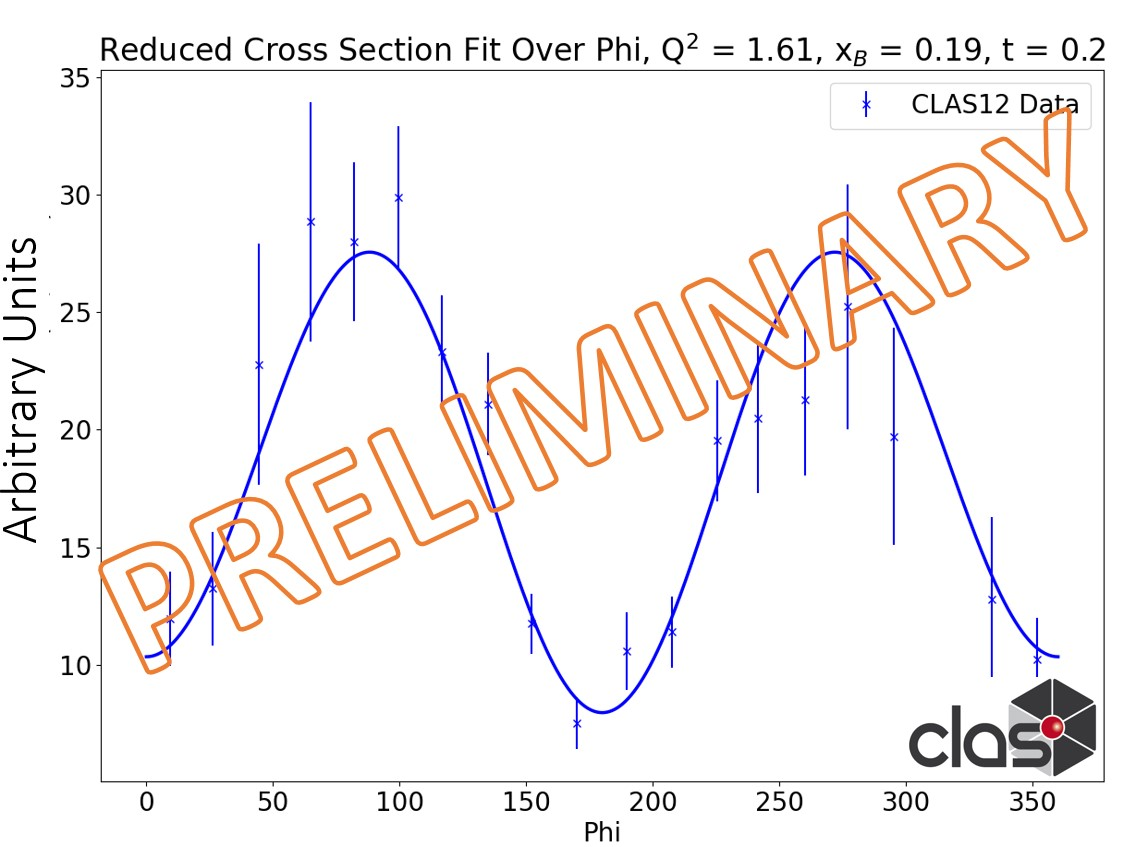
\includegraphics[trim={0 0  0 0cm} ,clip,width=.882\textwidth]{extra/xsec/fit1.jpg}
                   	\vspace*{-1.1cm}  % Tune this to the image height.
                    \begin{center}
                    \scalebox{.4}{\color{gray}*Err. bars stat. only          }
                    \end{center}
                    \vspace*{.2cm} 
                   	  
                	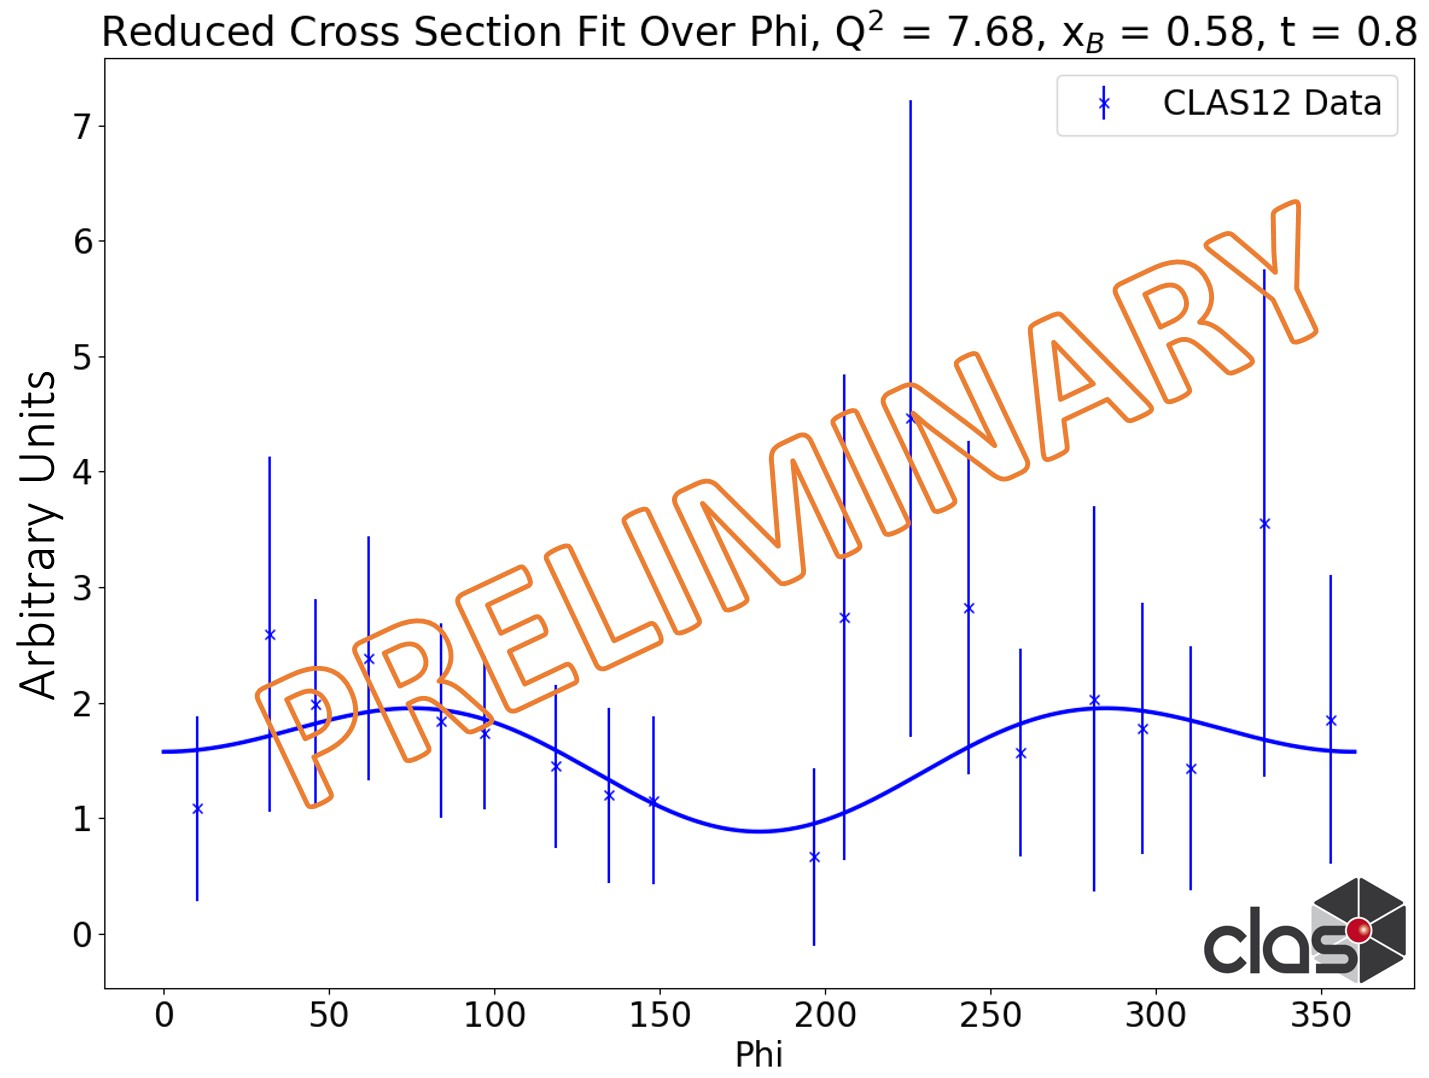
\includegraphics[trim={0 0  0 0cm} ,clip,width=.882\textwidth]{extra/xsec/xsec_7.jpg}
                	                   	\vspace*{-1.1cm}  % Tune this to the image height.
                    \begin{center}
                    \scalebox{.4}{\color{gray}*Err. bars stat. only          }
                    \end{center}
                    \vspace*{.2cm} 
       
                   \column{0.3\textwidth}
                %\textcolor{white}{blank space}
                     
            
                    %#---------------------------------------------
                   	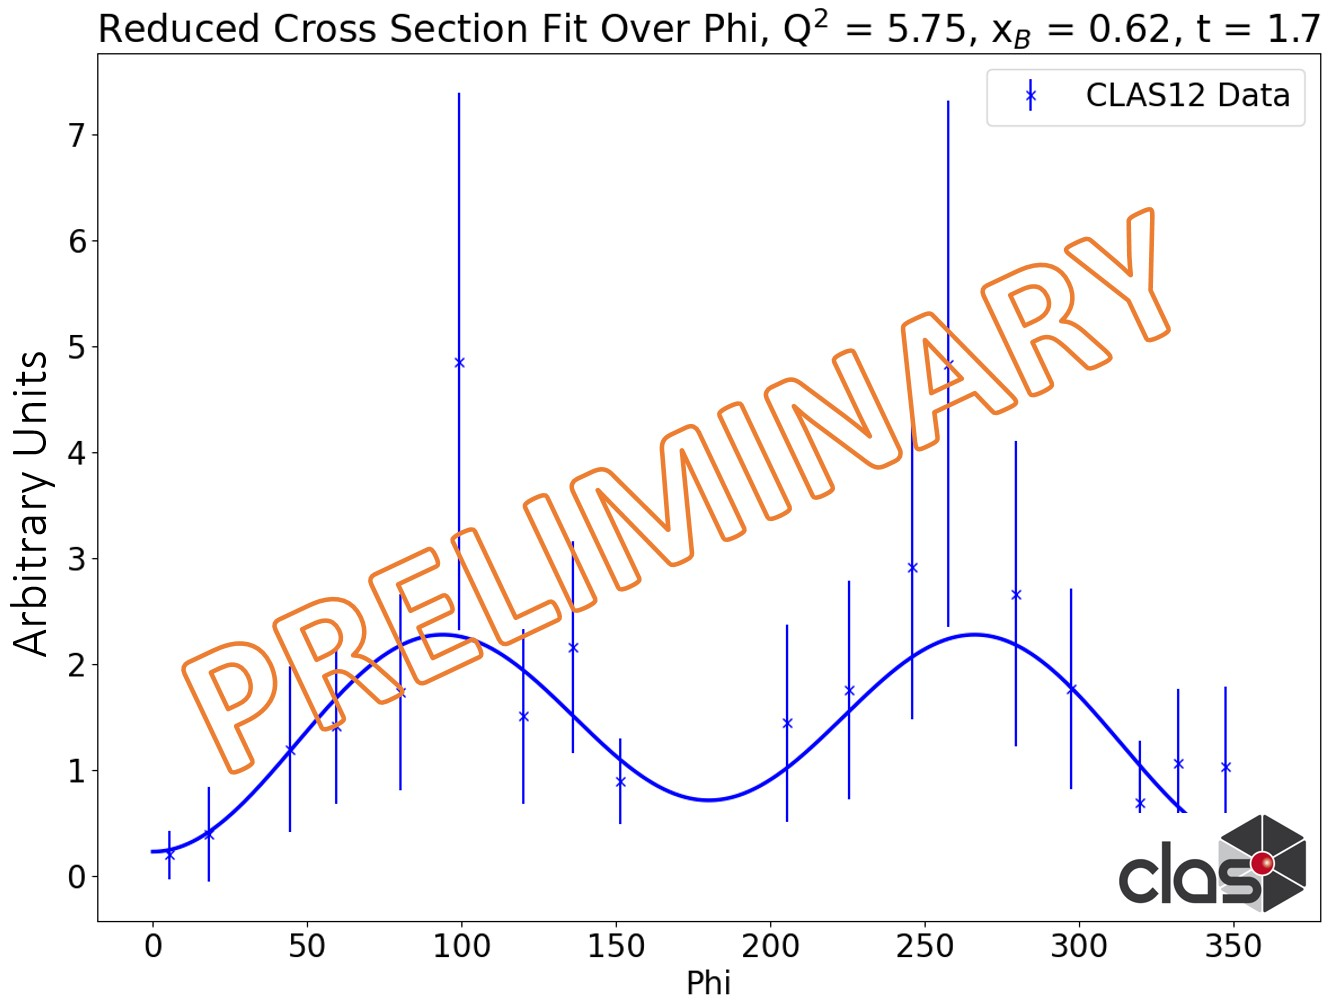
\includegraphics[trim={0 0  0 0cm} ,clip,width=.882\textwidth]{extra/xsec/xsec_5.jpg}
                   	                      	\vspace*{-1.1cm}  % Tune this to the image height.
                    \begin{center}
                    \scalebox{.4}{\color{gray}*Err. bars stat. only          }
                    \end{center}
                    \vspace*{.2cm} 
                    
                	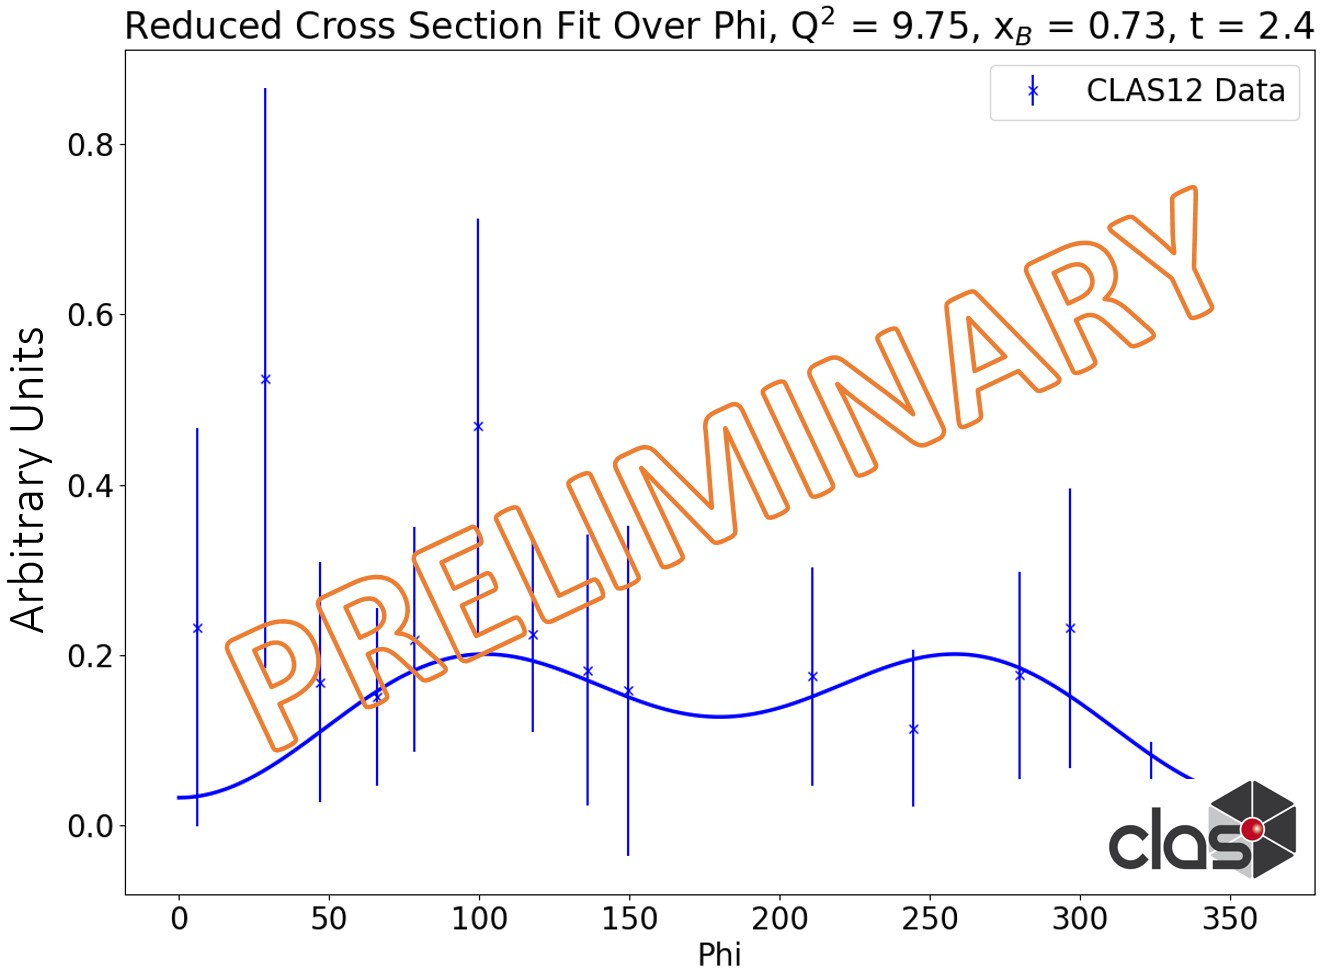
\includegraphics[trim={0 0  0 0cm} ,clip,width=.882\textwidth]{extra/xsec/xsec_9.jpg}
                	                   	\vspace*{-1.1cm}  % Tune this to the image height.
                    \begin{center}
                    \scalebox{.4}{\color{gray}*Err. bars stat. only          }
                    \end{center}
                    \vspace*{.2cm} 
       
       
       \end{columns}         	

\end{frame}



\begin{frame}{Theory Predictions - GK Model}
\begin{columns}[t, onlytextwidth]
            \column{0.4\textwidth}
            
                \begin{itemize}
                    \setlength\itemsep{1em}
                    \item \footnotesize Goloskokov-Kroll (GK) model predicts exclusive $\pi$ electroproduction cross sections using handbag approach\\
                    {\myfont{\tiny [S.V. Goloskokov $\&$ P. Kroll, EPJC, 65,137 (2010)]}}

                    \item Model parameters chosen to best describe recent CLAS $\pi^+$ BSA result\\
                    {\myfont{\tiny [S. Diehl et al., PRL 125 182001 (2020)]}}
                    
                    \item Software implementation from\\
                    K. Tezgin / PARTONS Framework\\
                    {\myfont{\tiny [B. Berthou et al., EPJC, 78, 478 (2018)]}}
                    
                    \end{itemize}
                    
                    \vspace{0.1cm}
                    \footnotesize Note: 
                    \vspace{0.1cm}
                     
                     \scalebox{0.835}{
                        W $>$ 2 GeV $\implies \frac{Q^2\left( 1-x_B\right)}{x_B} > 3.12$ GeV$^2$
                        }\\
                     
                     \scalebox{0.835}{
                            $t > t_{min} \implies t> \frac{m_p^2x_B^2}{1-x_B}$
                     }
                
                
            \column{0.3\textwidth}
            \centering
                Model Predictions\\
                	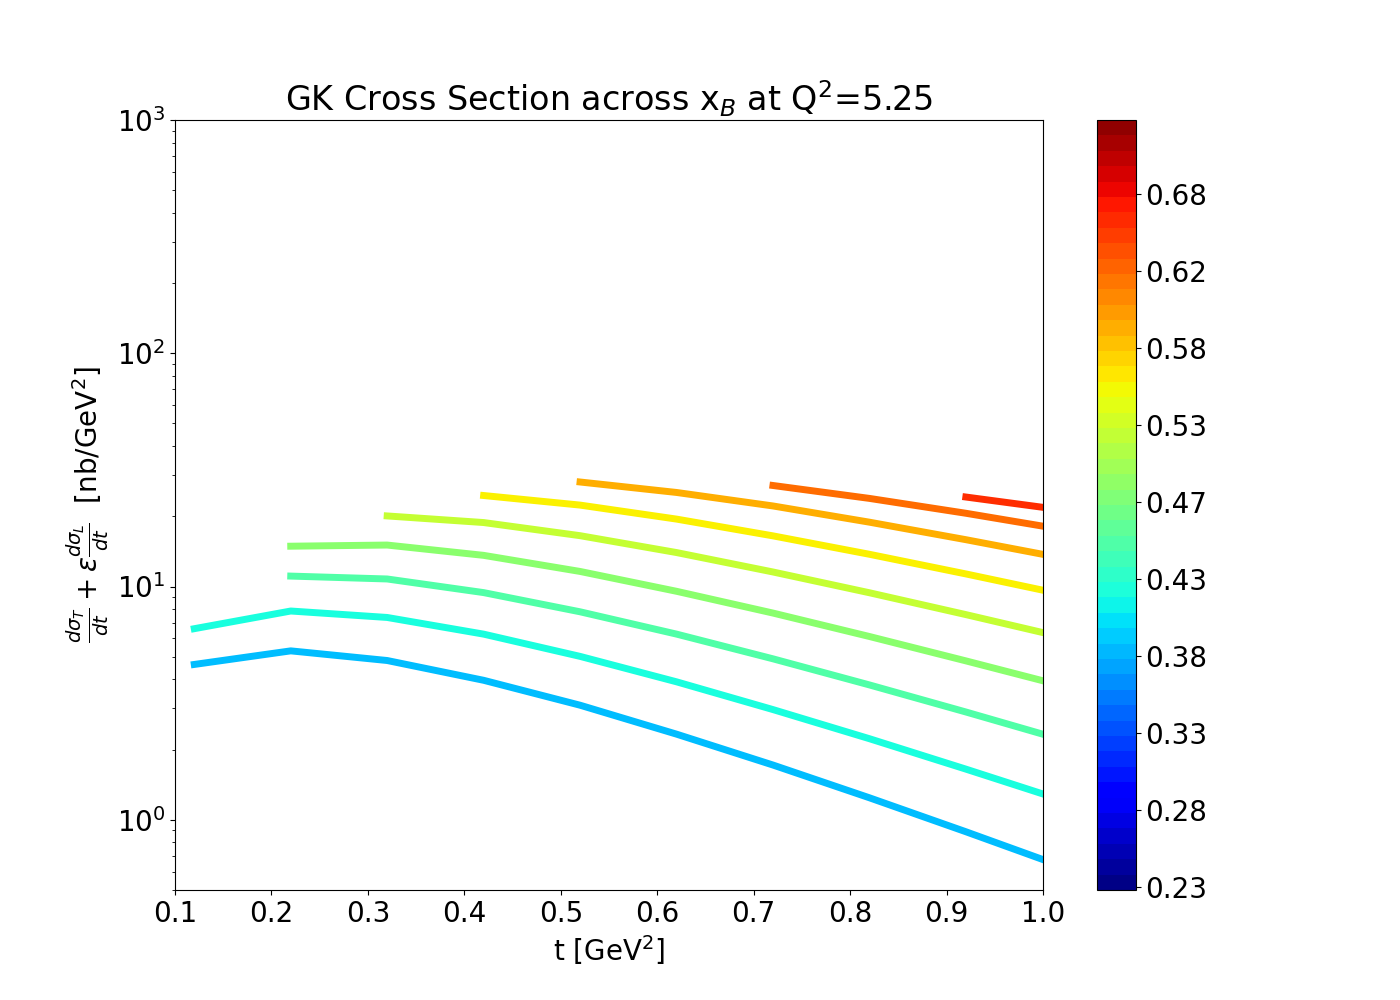
\includegraphics[trim={0 0  0 0cm} ,clip,width=.9882\textwidth]{DNP/gk_q2/fig_8_q2_5.25.png}
                	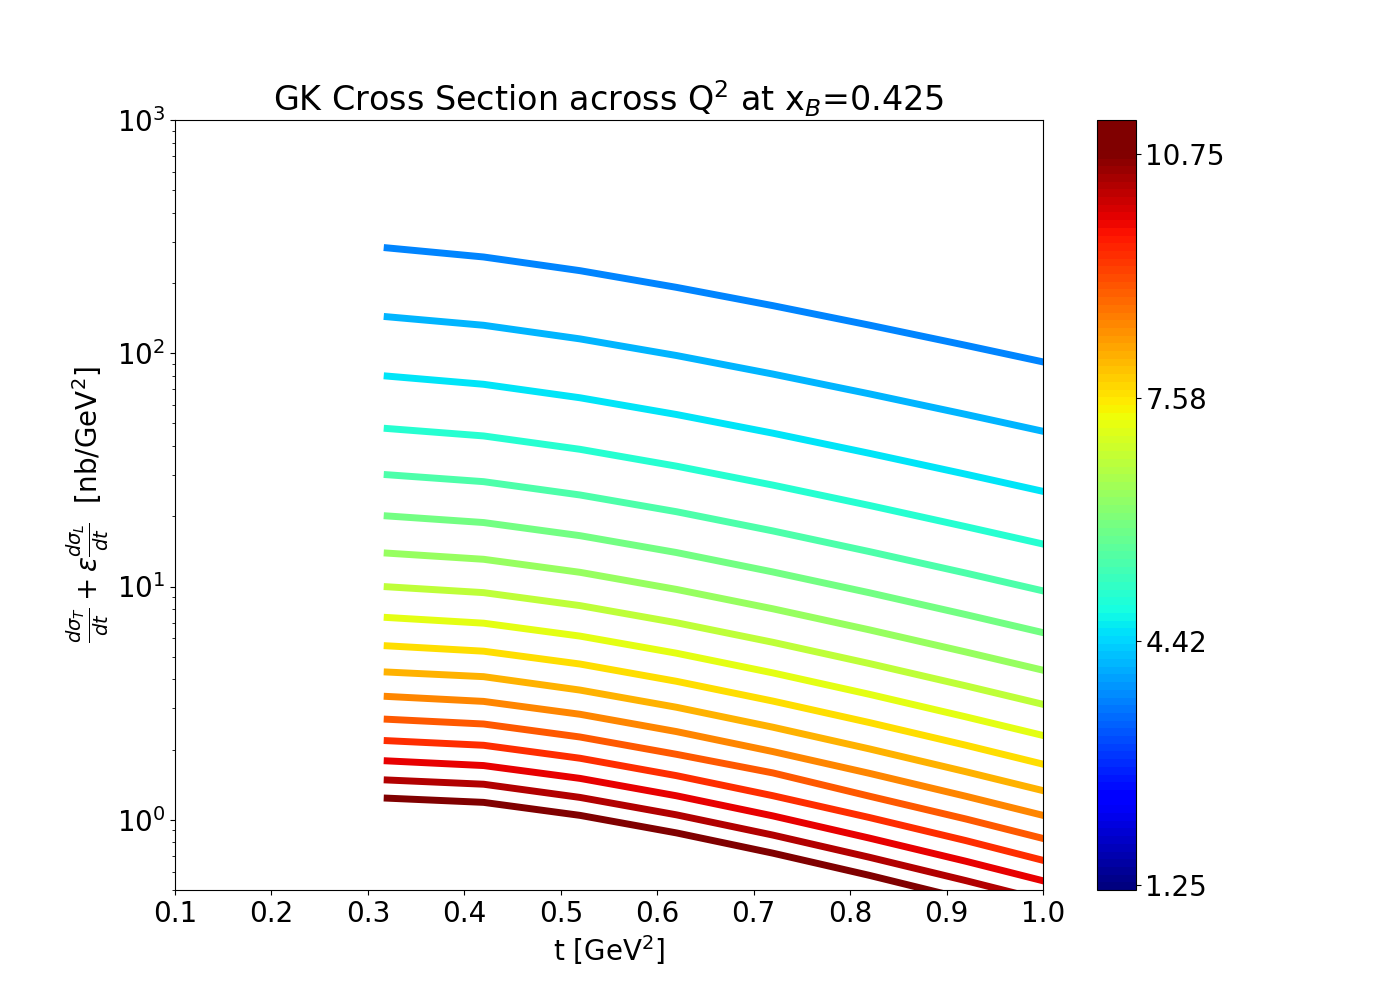
\includegraphics[trim={0 0  0 0cm} ,clip,width=.9882\textwidth]{DNP/gk_xb/fig_4_xb_0.425.png}
                		
            \column{0.3\textwidth}
                \centering
                \vspace{0.2cm}
                GK and CLAS12 Data
                    \includegraphics[trim={0 0  0 0cm} ,clip,width=.92\textwidth]{DNP/gk_1.jpg}
                    \vspace{0.1cm}
                	\includegraphics[trim={0 0  0 0cm} ,clip,width=.92\textwidth]{DNP/gk_2.jpg}
                		
                
        \end{columns}
\end{frame}



\begin{frame}{Finite Bin Volume Corrections}
Bin Average is not the same as bin center


\end{frame}


\begin{frame}{Ditching Binning - OMNIFOLD}
words

\end{frame}

\begin{frame}{Rosenbluth Separation}
Igor Paper

\end{frame}

\begin{frame}{Classifier -- box to manifold}
words

\end{frame}


\begin{frame}{Normalizing Flows}
words

\end{frame}

\begin{frame}{Simulation Based INference}
Words
\end{frame}

\begin{frame}{Conclusion - Towards a Full Cross Section}
Preliminary efforts on event selection, simulations, and acceptance corrections yield promising results but more work is needed to extract a complete cross section measurement:
\vspace{0.4cm}
\begin{itemize}
    \setlength\itemsep{1em}
    \item Determination of remaining correction factors - radiative, binning, and absolute normalization
    \item Study of systematic uncertainties 
    \item Quantitative comparisons between data and theory model will be meaningful when uncertainties and binning are more complete
\end{itemize}
    
%Acknowledge: MIT group, Sangbaek Lee, Andrey Kim, CLAS collaboration
\end{frame}
\begin{frame}{Acknowledgements}
MIT Milner Hadronic Physics Research Group: Richard Milner, Doug Hasell, Sangbaek Lee, Igor Korover, Xiaqing Li, Patrick Moran\\
CLAS Collaboration, Bates Engineering, MIT Tier 2 Computing Group
    
%Acknowledge: MIT group, Sangbaek Lee, Andrey Kim, CLAS collaboration
\end{frame}





\appendix



\begin{frame}{Extra slides}
Extra Slides

\end{frame}




\begin{frame}{Backup slides}
      - QCD factorization theorem for DVMP process has only been proven for longitudinally polarized photons\\
    - QCD factorization has been proven for DVCS
 
\end{frame}


\begin{frame}{Backup slides}

   \begin{columns}
            \column{0.5\textwidth}
            \includegraphics[scale=0.2]{Pics/currentWork/dvpipdiagram.png}\\
            DVMP is sensitive to chiral odd GPDs, distinguishing it from DVCS as a GDP probe\\
            
             \column{0.5\textwidth}
            \includegraphics[scale=0.14]{Pics/currentWork/cross-section-formula.png}\\
            \includegraphics[scale=0.085]{Pics/currentWork/gpds.png}\\
            
    \end{columns}
    
\end{frame}

\begin{frame}{Backup slides}
\centering
Comparision with CLAS6\\

    \includegraphics[scale=0.2832]{DNP/comp_c12_gk_c6.jpg}\\
\end{frame}

\begin{frame}{Backup slides}
\centering
Low Q2\\

    \includegraphics[scale=0.2832]{DNP/beauty_2.jpg}\\
\end{frame}

\begin{frame}{Backup slides}
\centering
Inbending

    \includegraphics[scale=0.2832]{DNP/nice_inbending.jpg}\\
\end{frame}



\begin{frame}{De-Fence!}
\centering
    \includegraphics[scale=0.5832]{Main/thesis_defense_2x.png}
    
    {\myfont{\tiny    https://xkcd.com/1403/   }}
\end{frame}


\begin{frame}{Backup slides}
\centering
Slide on cheesecake / pi
\end{frame}

\begin{frame}{Abstract}

Imaging the Proton: Investigating Proton Structure with Electron Scattering
\\
The structure of the proton has been studied extensively since its discovery a century ago.  Electron scattering experiments have been utilized as a clean probe into the dynamics of the nucleon, and the past several decades of work investigating structure functions have yielded information on the proton Parton Distribution Functions, which describe the proton's physical inner workings along one dimension. Presently, in specific kinematic regimes nuclear reactions can be theoretically linked to the 3D substructure of the nucleon. This presentation will discuss work towards measuring the properties of one such reaction - Deeply Virtual Neutral Pion Production - from analyzing the data of a 10.6 GeV electron scattering experiment at the CLAS12 detector in Jefferson Lab Hall B. 

\end{frame}


\begin{frame}{Backup slides}
Comments on measuring pion polariability
a few words about how pions are useful
\end{frame}

\begin{frame}{Backup slides}
\centering
Other\\

    \includegraphics[scale=0.2832]{DNP/finalfig2.png}\\
\end{frame}


\begin{frame}{Concrete Abstract}

The structure of the proton has been studied extensively since its discovery a century ago.  Electron scattering experiments have been utilized as a clean probe into the dynamics of the nucleon, and the past several decades of work investigating structure functions have yielded information on the proton Parton Distribution Functions, which describe the proton's physical inner workings along one dimension. Presently, in specific kinematic regimes nuclear reactions can be theoretically linked to the 3D substructure of the nucleon. This presentation will discuss work towards measuring the properties of one such reaction - Deeply Virtual Neutral Pion Production - from analyzing the data of a 10.6 GeV electron scattering experiment at the CLAS12 detector in Jefferson Lab Hall B. 

\end{frame}


\begin{frame}{Backup slides}
\centering
    Find this online at: https://github.com/robertej19/Thesis-Offense/blob/main/presentation.pdf
\end{frame}


\end{document}